\documentclass[11pt,openany,oneside]{book}
\usepackage[left=1in,right=1in,top=1in,bottom=1in]{geometry}
\usepackage{setspace}
\usepackage{indentfirst}
\usepackage{multirow}
\usepackage{enumitem}
\usepackage{booktabs}
\usepackage{tabularx}
\usepackage{natbib}
\usepackage{graphicx}
\usepackage{caption}
\usepackage[colorlinks=true,allcolors=black]{hyperref}
\usepackage[nottoc,notlot,notlof]{tocbibind}

%\usepackage[draft,nomargin,marginclue,footnote,index]{fixme}
%\newcommand{\fix}[2]{\fxnote*{#1}{#2}}

\newcommand{\dtitle}{Doing ``Good" with Data? Understanding and Working Around Data Doubles in Human Services Organizations}

\begin{document}
\frontmatter
\doublespacing

%Title Page
\thispagestyle{empty}
\begin{center}
\begin{minipage}{\linewidth}
    \centering
	\vspace{3cm}
	{\Large\MakeUppercase{\dtitle}\par}
	{\large by\par}
	{\uppercase{\Large Chris Bopp\par}}
	%{\Large CHRIS BOPP\par}
	{\large B.S., Rochester Institute of Technology, 2006\par}
	{\large M.S., University of Colorado Boulder, 2015\par}
	\vspace{3cm}
	{\large A thesis submitted to the\\Faculty of the Graduate School of the\\University of Colorado in partial fulfillment\\of the requirement for the degree of\\Doctor of Philosophy\\Technology, Media, \& Society\\2020\par}
	\vspace{1cm}
\end{minipage}
\end{center}

\begin{flushright}
\begin{minipage}{\linewidth}
\raggedleft
	{\large Committee Members: \par}
	{\large Dr. Amy Voida\par}
	{\large Dr. Lehn Benjamin \par}
	{\large Dr. Geoffrey Bowker \par}
	{\large Dr. Leysia Palen \par}
	{\large Dr. Danielle Varda \par}
\end{minipage}
\end{flushright}
\clearpage


%Signature Page
% \thispagestyle{empty}
% \singlespacing
% \begin{center}
% \begin{minipage}{0.80\linewidth}
%     \centering
%     \vspace{2cm}
% 	This thesis entitled:\\
% 	\vspace{0.3cm}
% 	\dtitle\\
% 	\vspace{0.3cm}
% 	written by Chris Bopp\\
% 	\vspace{0.3cm}
% 	has been approved for the ATLAS Institute\\
% 	\vspace{1cm} \rule{8cm}{.5pt}\\
% 	Dr. Amy Voida, Chair\\
% 	\vspace{1cm} \rule{8cm}{.5pt}\\
% 	Dr. Lehn Benjamin\\
% 	\vspace{1cm} \rule{8cm}{.5pt}\\
% 	Dr. Geoffrey Bowker\\
% 	\vspace{1cm} \rule{8cm}{.5pt}\\
% 	Dr. Leysia Palen\\
% 	\vspace{1cm} \rule{8cm}{.5pt}\\
% 	Dr. Danielle Varda\\
% 	\vspace{1cm} \underline{\hspace{2.5cm} June 12th, 2020 \hspace{2.5cm}}\\
% 	Date\\
% 	\vspace{1cm}
% 	The final copy of this thesis has been examined by the signatories, and we find that both the content and the form meet acceptable presentation standards of scholarly work in the above mentioned discipline.\\
% 	\vspace{1cm}
% 	IRB Protocols: \#15-0553, \#19-0575
% \end{minipage}
% \end{center}
% \clearpage
% \doublespacing

%Abstract Page
\thispagestyle{plain}
{\large \noindent Bopp, Chris (Ph.D., Technology, Media, \& Society)\par}
{\large \noindent \dtitle\par}
{\large \noindent Thesis directed by Assistant Professor Amy Voida\par}
\vspace{1cm}
Over a third of US federal spending is dedicated to providing critical human services such as workforce development, public health education, and child welfare. Under the federalist system, decision making authority is shared by the federal, state, and local governments thereby decentralizing responsibility for the delivery of social services across multiple levels of government and implementing nonprofit organizations. The distributed nature of this decision making means that decisions happen within and across multiple levels: at the individual level during client meetings, at the organizational level within one or more human service organizations during the evaluation of a program, at regional- or state- level coordination task force meetings, and during federal-level legislative hearings. For the individual client’s experience to be legible at higher levels of aggregation, institutions and organizations prescribe standardized measures and categories to represent the client as a data double.

In this research, strategies and approaches to work with and around data doubles are examined in the context of interorganizational human services. This work focuses on the stakeholders that have varying degrees of power, the infrastructure with its expectations for translating the world into data schemas, and the broader values and politics that shape both of these. The dissertation is comprised of three empirical chapters which focus on understanding 1) the sociotechnical system, 2) the way that data is aggregated using unique identifiers, and 3) the way that data is used to answer diverse stakeholder questions. Together, this empirical work contributes a detailed analysis of data work across multi-level computer supported cooperative work in the human services domain. This research illustrates that in order to support the kinds of innovative uses of big data that many desire in the social sector, more diverse stakeholders need to be involved in the design and implementation of data systems so that they may better meet the needs of clients, staff, and the community.

\clearpage
 
%Acknowledgement Page
\thispagestyle{plain}
{\Large \noindent \textbf{Acknowledgments} \par} \vspace{.5cm}
This dissertation would not have been possible without the involvement of human services staff and volunteers---who have committed their lives to helping others---as well as individuals who seek this assistance. Thank you for participating in this research, and I hope that I have not only authentically reflected your experiences, but that this research can be used to advocate for change.

I also would like to thank Dr. Tara Walker for not only helping me persevere through the challenges of completing a PhD but for inspiring me to pursue my passion in the first place. You gave me the courage to take the risks that I needed to take to become the person I have always wanted to be. You've encouraged me to embrace uncertainty and complexity in the face of my natural inclination towards order and certainty. Rather than shutting down my curiosity about the world, you've always encouraged me to dig deeper no matter where that may take me. I am so incredibly fortunate to have such a wonderful person as not only my wife but also as a colleague.

Two other people who have been instrumental in encouraging me to pursue this research are Dr. Revi Sterling and Dr. Leysia Palen. In my master's program, both Revi and Leysia sparked a curiosity in me that could not be extinguished. As I neared the end of the short two-year program, both Revi and Leysia encouraged me to continue pursuing my interests and for that, I am incredibly grateful. To this day, I am constantly astounded that Leysia---someone for whom I have the ultimate respect---saw something promising enough in me to employ me as a research assistant in her lab, which kicked off my research career.

And of course, I could not have completed this research without the support of Dr. Amy Voida, my doctoral advisor. I am fortunate to have had such a passionate individual to geek out with on a regular basis. I have learned so much from you and have grown in so many ways as a researcher, teacher, and collaborator as a result of your meticulous advising. I am amazed at your ability to not only understand my passion (often before I do myself), to see the path forward, and to support me in coming to a conclusion myself. It wasn't always efficient or easy, but you somehow found a way to strike a balance between giving me advice and letting me learn for myself. Thank you for your dedication and support over the years, I could not have done this without you.

Finally, none of this would have been possible and I would not be where I am today were it not for my parents. You emphasized the importance of education and made sure that I worked hard towards earning my bachelor's degree. I know that the education I've pursued since then and the decisions that I've made haven't always seemed the most practical, but you've both always supported me unconditionally and for that I am grateful.
%\clearpage

\pagestyle{plain}
\tableofcontents
\listoftables
\listoffigures

\mainmatter

\singlespacing \chapter{Introduction} \label{ch:intro}
\doublespacing \chapter{Introduction}
\label{ch:intro}

% Robin's comments
    % more structure: subsections, giant block of text.
    % better argument for your case
    % the result of the arguments should be the research questions
    % some alternatives of the research questions

% \todo[inline]{should I talk about information need of users and the fundamentals why recommender systems are a service and what they are? I don't do that here at all.}
% \todo{research context}

After a fast development in creating ``smarter'' digital systems, more and more decisions are being delegated to algorithms. Having observed the evolution, influence, and consequences of these AI-supported systems over time, concerns have been grown in the public discourse about ethical issues and the potential harms of these systems to individuals and society. 
% Machine learning is and continues to be one of the main pillars of these systems.
 
Recommender systems are one of the most pervasive applications of AI/machine learning. They play a pivotal role in connecting users to relevant items or content throughout the web. Not only do users rely heavily on these systems, but also other parties such as content producers, sellers, or information providers. Although these systems are intended to assist people in different tasks, they can risk implicit or explicit discrimination against individuals or groups, especially marginalized groups. Consider a recommender system suggesting job opportunities to job seekers. Discriminatory recommendations in these systems could mean that men and women with similar qualifications don't get recommendations for jobs with equal rank and salary.
%they can potentially cause implicit or explicit

% \todo[inline]{is a job recommendation scenario out of context?}
% Many online... is redundant.

%Many online platforms attempt to connect job opportunities and job applicants in some way.Sometimes they are professional networks with a job-seeking component such as Xing and LinkedIn, or they might have been designed only for employment seeking.

For example, suppose more women apply for lower-paying jobs on a given job-seeking website, and the recommendation algorithm learns the correlation between demographic information and job salaries. Jobs with lower salaries or ranks might show up more often in the recommendations to women and jobs with better salaries and higher ranks will be recommended to men. Basileal et al. (2021) \cite{Korolova2021JobAds} demonstrate this issue in the Facebook's ad delivery system and how demographic information causes the system to discriminate against women regardless of their qualifications.

%not recommender system's fault!
% In another real-world example, Brian Stauffer (2018) from Human Rights Watch reports similar discrimination against women in the job market \cite{HRW2018ads}. They analyzed over 36,000 job advertisements posted between 2013 and 2018 on Chinese recruitment and company websites and social media platforms. Many of the ads specify a requirement or preference to hire men regardless of other qualified women candidates. Some job posts require women to have certain physical attributes – with respect to height, weight, voice, or facial appearance – that are irrelevant to job duties.

% ali2019JobDiscrimination
% when they get similar recommendations, it is just because of their demographic information not because of their qualifications.

Now, consider a loan recommender system that suggests loans to lenders to support. Many online platforms attempt to connect small businesses or entrepreneurs in need of loans to lenders or donors, such as Kiva.org or DonorsChoose.org. Discriminatory recommendations in these systems could mean that, for instance, more attractive, lighter-skinned, and less obese borrowers are favored (discussed by Christina Jenq et al. (2015) \cite{JENQ2015234}), and their loans get funded faster.

There are several ways that different biases can creep into recommender systems. Reflection of societal and historical prejudices in datasets, lack of data on minority groups or any problem in data collection, and lack of suitable model designs and evaluation methods are among the underlying reasons for unfairness in these systems. A system needs to defend against these biases in recommendation output, even biases that arise due to behavioral differences. For example, male users might be more likely to apply optimistically for high-paying jobs compared to women. These differences reflect how these biases might have been internalized in people in the society and their behavior which may lead to discrimination in job recommendation. 


% \section{Running example}
% \todo{expand on it}

% \todo[inline]{
% Microlending is the provision of small and low-interest loans (as little as \$25) to low-income individuals or small-scale entrepreneurs from under-developed countries \cite{yunus1998banker}. The extremely poor people in rural areas often lack collateral, steady employment, or a verifiable credit history, hence they cannot get access to financial services. Under such circumstances, microlending has attracted an increased attention in the last decade \cite{chen2017microfinance}, providing impoverished entrepreneurs an opportunity to start their own businesses as well as avoid the vicious cycle of debt.

% One of the leading international microlending organizations, Kiva Microfunds (Kiva.org), has crowd-funded about 3 million borrowers with \$1.27 billion USD as of February 2019 \cite{kiva}. Kiva does not collect interest but provides an intermediary service for lenders and borrowers, as illustrated in Figure \ref{fig:kiva_process}. Borrowers from over 80 countries, divided into 8 regions by Kiva, post their applications for loans on the website for lenders to support. Lenders browse and crowd-fund the loans in the increments of \$25 or more. }

% Consider a loan recommender system that suggests loans to lenders to support. There are many online platforms attempting to connect small businesses or entrepreneurs who have requested for a loan to lenders or donors in some way. Discriminatory recommendations in this system could mean that for instance, more attractive, lighter-skinned, and less obese borrowers are favored \cite{JENQ2015234}, and their loans get funded faster. 
% Or when they get similar recommendations, it is just because of their similar demographic information not because of reasons they have provided about why they need the loan.

% The system would therefore need to defend against biases in recommendation output, even biases that arise due to behavioral differences: for example, certain regions in the world are more favored due to the historical or political relationships of the countries where the lenders and borrowers reside. Therefore, certain borrowers unjustly get a high exposure to the lenders and the others might not get any visibility at all. And due to the formed positive feedback loops, this gap might get wider over time, resulting in ignoring certain user subgroups.

% Consider a recommender system suggesting job opportunities to job seekers. Many online platforms attempt to connect job employments and job applicants in some way. Sometimes they are professional networks which have a job-seeking component such as Xing and LinkedIn, or they might have been designed only for employment seeking.

% Discriminatory recommendations in this system could mean that men and women with similar qualifications don't get recommendations of jobs with similar rank and salary. Or when they get similar recommendations, it is just because of their demographic information not because of their qualifications. For examples, if there are more women on a job recommendation website and they all apply for secretarial jobs, these jobs might show up in the recommendations of women who are looking for CEO jobs. On the other side of the coin, jobs with better salaries and higher ranks will be recommended to men regardless of their qualifications. The system would therefore need to defend against biases in recommendation output, even biases that arise due to behavioral differences: for example, male users might be more likely to click optimistically on high-paying jobs. \todo{more clarifications?}

% \section{Sources of unfairness in recommender systems}

% % potential underlying reasons for recsys to be unfair
% Multiple underlying reasons cause the recommendation algorithms to be unfair. For example, if recommender systems are trained on biased data, the outcomes might get biased, a.k.a. "garbage in, garbage out."

% These algorithms might also propagate the existing biases in the data \cite{barocas2016big}. For example, recommender systems increase the popularity of items by just presenting those items to the users. 
% It is known that these systems affect the users’ opinion, and hence, their ratings of items \cite{Cosley2003Influence}. Thus, a user’s rating of an item is either their intrinsic preference or the influence of the recommender system on the user. Users are more likely to click on the items that recommender systems deliver to them. This phenomenon is called presentation bias \cite{baeza2018bias}. 

% Over time, items gain even more popularity as they are shown to users, up to the point that less popular items are not recommended at all. Due to the positive feedback loop, the item space shrinks, and the recommendation lists become too homogeneous \cite{Chaney2018Homogeneity}. The formed \textit{filter bubble} might be harmful or unfair to users as users' choices become limited and homogeneous, preventing them from novel content or ideas.

% A real-world example of the harms that filter bubbles cause; is the influence of the news feeds on people's minds that can eventually lead to political polarization~\cite{HONG2016777}. Not only is this issue discriminatory towards users, but it is also unfair to (content) providers as a small group of them gain unfairly high visibility while the others are systematically pushed away. In a music streaming platform, this issue could affect the livelihood of musicians. In Algorithms of Oppression, Sofiya Noble \cite{noble2018algorithms} discusses this issue in personalized search through real-world examples and people's experiences. The author later, discusses how popularity bias in Yelp along with other factors such as private interests in promoting certain sites, along with the monopoly status of a relatively small number of Internet search engines, can potentially lead to racial discrimination, especially businesses owned by women of color.

% Over-personalization in Youtube's recommendation algorithms has also caused harm to suicidal teenagers by showing them similar videos on different ways of committing suicide.
% This type of bias occurs because users are more likely to interact with items that the system presents to them. 
    
% The first issue here is the item selection by the recommender system here and whether it will contribute to unfairness to any of the stakeholders. We have addressed how to mitigate this issue in Chapter \ref{fairness} in the pre-processing section \todo[inline]{preprocessing section}. 
    
% The second issue is that presentation bias, can lead to a form of positive feedback loop, in which presented items gain more popularity since they are more likely to be interacted with. This leads to greater bias towards presenting the items when the popular items are promoted more at the cost of other items. Presentation bias and the created feedback loop not only magnifies the initial differences between items' popularity but also it makes it hard for new providers to attract the attention of users to their products/items in a system with this type of bias.
    
% For example, in the microlending case, if the system doesn't recommend loans from a specific geographical region because on average the requested loans from this region are risky (their borrowers are less likely to return the loan), not only the current good borrowers (the borrowers who are more likely to return the loan) from that region are affected, but also the future good borrowers. This positive feedback loop reinforces over time until that region is completely ignored by the system.

\section{Fairness-Aware Recommender Systems}

Disregarding the societal impacts and ethical consequences of recommendation algorithms in different applications leads to algorithm designs that are unfair or harmful to their users. In recent years, the topic of fairness in machine learning has gained the attention of a multi-disciplinary community from computer scientists, social scientists to legal scholars. Thus as a response, recent research has shifted from design of algorithms optimizing for accurate outcomes to ones that also consider algorithms' social impacts. 
% such as representational or distributional harms. %accurate outcomes 

The problem of mitigating unfairness in recommender systems has unique challenges that set it apart from general machine learning fairness problems: (a) the multi-stakeholder nature of these systems and (b) the centrality of personalization and its trade-off with fairness goals. These two unique properties prevent the researchers from directly translating the proposed solutions and common techniques in machine learning fairness to recommender systems. In the following sections, we dive into each of these two points separately.


\subsection{Fairness in Multi-stakeholder Systems}

Recommender systems are often multi-stakeholder settings with users or consumers (of recommendations), providers or producers (of content/items), or other parties involved in systems transactions. Fairness concerns might arise for any of these stakeholders, such as consumers, referred to as \textit{consumer-side fairness} concerns, or providers, referred to as \textit{provider-side fairness} concerns, or other stakeholders.

As an example, a system might be discriminatory towards certain job-seekers (consumers), such as women, by presenting them the recommendations of lower-paying job opportunities based on their demographic information, or it could be unfair to certain businesses (providers), such as start-ups, by not giving them enough visibility to the best candidates. In certain applications, these concerns might need to be addressed at the same time, but achieving universal fairness for all is impossible \cite{friedler-impossibility-2021}. So, we might need to prioritize fairness concerns across different stakeholders.


\subsection{Personalization versus Fairness}
% what accuracy is? and what word should we replace it with?
% In machine learning algorithms, achieving optimum accuracy by itself is impossible and might not even be desirable!

% I think you need to start with definitions: first, fairness. What do you mean? I would say the definition is something like: “The output of the system conforms to some normative distributional properties with respect to particular stakeholders.” Next, accuracy. “A system gives accurate recommendations if it can, on average, reproduce the preferences of users expressed in historical ratings data.” Don’t rely on people’s common-sense ideas of these terms, since you really mean something quite specific.

% With definitions in place it is easier to describe the tension between them: the historical preferences of users might not match the desired normative properties; the historical ratings of users are themselves only uncertainly related to users’ preferences; the historical ratings data is contaminated with various kinds of biases; the desired distributional properties work to the benefit of subgroup but the accuracy measure is averaged over all users; etc.

Traditionally, the main goal of a recommender system is personalization. In other words, recommender systems strive to present items to the users that are tailored to each user's taste and are more likely to be interacted with. To achieve personalization, these systems utilize users' historical log data to produce accurate recommendations. A system has high \textit{accuracy}, if it can, on average, reproduce the preferences of users expressed in historical ratings data.

A system is \textit{fair} if the output of the system conforms to some normative distributional properties with respect to particular stakeholders. Achieving a balance between fairness and accuracy as defined previously is challenging due to their intrinsic tension. The major underlying causes of this tension are as follows: the historical preferences of users might not match the desired normative properties; the historical ratings of users are themselves only uncertainly related to users’ preferences; the historical ratings data is contaminated with various kinds of biases; the desired distributional properties work to the benefit of subgroup but the accuracy measure is averaged over all users; etc. Below, I discuss an example for each cause.
% \todo[inline]{the topics needs to change - no time though :|}


% Based on this definition, achieving optimum accuracy by itself is impossible because the historical preferences of users might not match the desired normative properties. 

% Additionally, optimizing for accuracy might reinforce the popularity bias or some consumer-side unfairness. The following sections discuss how optimizing for accuracy can lead to user dissatisfaction and why we might need to balance accuracy with other system goals, such as fairness.

% \vspace{0.25cm}
% \noindent \textbf{(\romannum{1}) Fairness}
% \vspace{0.25cm}


% \subsection{Impossibility of Ideal Accuracy}
\vspace{0.25cm}
\noindent \textbf{(\romannum{1}) Impossibility of Ideal Accuracy}
\vspace{0.25cm}

Recommender systems recognize the more general patterns in the data and use this information to predict users' rating behavior for recommendation generation. These general patterns are based on historical logged user interactions with the system. Therefore accuracy for recommender systems is fidelity to historical patterns in the data and the ability to reproduce users' exact preferences. 

However, human behavior is always associated with some degree of uncertainty (as Hill et al. (1995) explains in \cite{hill1995recommending}), which will lead to deviation from perfect accuracy. This uncertainty might originate from the natural variability of human decision-making, or it might be system-induced. Users' rating behavior is inconsistent, and their preferences are not fixed. Said et al. (2012) \cite{Said2012MagicBarrier} introduces and discusses the concept of the \textit{magic barrier} in recommender systems, a barrier caused by variability in user behavior which prevents the model from reaching an ideal accuracy. Besides the behavioral inconsistency, users' tastes might evolve as they consume the recommendations. McAuley et al. (2013) \cite{McAuley2013expertise} discuss how user's ratings of beers change as their palate tastes more complicated tastes over time. 

% \todo[inline]{what the users want and what they click on is different?}
%historical logged user


% In this case, recommender systems generate recommendations according to the general patterns of users interests. 

To improve accuracy, recommender systems might need to model these temporal and dynamic changes. Additionally, recommender system models built on general patterns in the data capture mainly the long-term interests of users and might disregard users' short-term needs and interests. Many researchers, including Adomavicius et al. (2011) \cite{Adomavicius2011context}, have attempted to use contextual information to account for these changes.

In some cases, due to technical limitations or lack of data, the system fails to present users their items of interest, so users might end up clicking on the items that are not reflective of their interest. This data might enter the training data and bias the input for the subsequent iterations. The points mentioned above are just a few examples of underlying confounding factors behind variability in user behavior that make the prediction task challenging in these systems.

Even if the users' behavior is consistent and ideal accuracy is reachable, users' preferences might not conform to fairness concerns. This might be because users are inherently biased or simply because users are unaware of the unfairness in a system. As an example, Kiva.org's lenders might not be aware of the unprivileged borrowers in the system. Therefore, supporting loans only based on their preferences might further exacerbate the unfairness of capital distribution in the system.

% This is partly because users' 
% to keep up with the variability in users' rating behavior
% Users' preferences are inconsistent.
%These changes are hard to predict as there are many underlying confounding factors involved in them.

%  Some authors speculated that we may be reaching
% some Magic Barrier where this variability prevents us from getting much more accurate

% In practice, it is hard to predict the information need of users at each point in time. 
% In fact, users themselves might not even know what they want. For example, It would be odd to think that every time a user opens a music streaming platform, she will exactly know the songs she wants to play. So, achieving ideal accuracy is unlikely in spite of optimizing the objective function to increase it.

% For example, when you want to listen to music, a lot of the times you don't think about the songs you exactly want to listen to. You might not want to listen to what you were listening before. Therefore, we can never achieve perfect accuracy and presenting accurate recommendations to the users is a myth.

% Below are some examples of the potential biases that increasing accuracy causes for consumers and providers.
% \todo[inline]{check all the biases mentioned before..}

\vspace{0.25cm}
\noindent \textbf{(\romannum{2}) Accuracy and Data Imbalance}
\vspace{0.25cm}
% \subsection{Accuracy \& Data Imbalance}

The collected data used for training recommendation models might not reflect the diversity in the society due to various reasons such as biases in data collection or simply lack of online participation from minority groups. These issues can create data imbalance leading to accuracy imbalance between the majority user group(s) for whom we have more data versus minority groups with less data. Since accuracy-based metrics are aggregated over all the users, they may fail to capture the accuracy for different user subgroups in a system. Usually, accuracy reflects the quality of the recommendations that the majority of the users experience regardless of other minority groups' experience. The error disparity for different user groups is considered a type of unfairness and trying to balance it is of interest for the research community \cite{ekstrand2018all,yao2017beyond}.

% Therefore, minority groups might not receive a high-quality service in the system.

% These metrics are usually averaged over all the user base and skewed towards the majority user group.   So, having a discrepancy in recommendation quality for different user groups is a type of unfairness in recommender systems and reaching to balance it, is of interest for the research community \cite{ekstrand2018all,yao2017beyond}.

\vspace{0.25cm}
\noindent \textbf{(\romannum{3}) Accuracy and Popularity Bias}
\vspace{0.25cm}
% \subsection{Accuracy \& Popularity Bias}
% how is accuracy and popularity related
% \todo[inline]{define accuracy}

Recommendation datasets are usually intertwined with popularity bias \cite{celma2008hits,lee2014fairness}. Striving to reach high accuracy will often lead to reinforcing popularity bias~\cite{barocas2016big}. It is known that these systems affect users’ opinions, \cite{Cosley2003Influence}. Thus, a user’s rating of an item might be their intrinsic preference, or based on the influence of the recommender system, or a combination of both. Users are more likely to click on the items that recommender systems deliver to them. This phenomenon is called \textit{presentation bias} \cite{baeza2018bias}.

Over time, items gain even more popularity as they are shown to users, up to the point that less popular items are not recommended at all. Due to this positive feedback loop, the item space shrinks, and the recommendation lists become too homogeneous \cite{Chaney2018Homogeneity}. The formed \textit{filter bubble} might be harmful or unfair to users as users' choices become limited and homogeneous, preventing them from receiving novel content or ideas. A real-world example of the harms that filter bubbles cause for users is the influence of the news feeds on people's mindset that can eventually lead to political polarization~\cite{HONG2016777}.

% These algorithms might also propagate the existing biases in the data \cite{barocas2016big}. For example, recommender systems increase the popularity of items by just presenting those items to the users.

% Not only is this issue discriminatory towards users, but it is also unfair to (content) providers as a small group of them gain unfairly high visibility while the others are systematically pushed away. 
Not only the consumers of recommendations will be affected, but the item providers might also suffer from discrimination. Popularity bias leaves less popular (item) providers with fewer consumer exposure opportunities, pushing them away from the system. This unjust exposure can affect their livelihoods. In a music streaming platform, this issue could affect the musicians income. 

The unfairness caused by systems is not equally harmful to that system's users. It usually puts a greater burden on the protected groups, particularly those who sit at the intersection of multiple protected attributes, such as ``new'' businesses owned by ``women'' of ``color''. In \textit{Algorithms of Oppression}, Sofiya Umoja Noble (2018) \cite{noble2018algorithms} discusses this issue in personalized search through real-world examples and people's experiences, including how popularity bias in Yelp along with other factors such as private interests in promoting certain sites, as well as monopoly status of a relatively small number of Internet search engines, can potentially lead to racial discrimination, especially businesses owned by women of color.

Popularity bias in the input data can lead to defective power dynamics in the user subgroups and influence the overall recommendations. As an example, Eskandanian et al. \cite{Eskandanian2019power} discusses how this issue can cause the preference of 95\% the users to be overshadowed by only the preference of 5\% of influential users who have rated mostly popular items (consumer unfairness).

Using accuracy as the only measure to optimize might even be undesirable or unsatisfactory to one or all the stakeholders of a recommender system. This is because increasing accuracy, without considering other goals and the potential causes of harm, can contribute to introducing and propagating biases or even reinforcing some of the existing biases in the system, such as popularity bias, positive feedback loops, filter bubbles, miscalibration error, over/under estimation of the predictions, etc. 


% Recommendation datasets are usually inter-weaved with popularity bias. Striving to reach a high accuracy will lead to reinforcing popularity bias as well. Over time, this bias gets even worse due to the effect of positive feedback loops in the system.

% As a result, popular items will gain more popularity and will be recommended more often. 
% Therefore users will receive more and more homogeneous recommendations over time. The created filter bubble and presenting users with limited options is unsatisfactory to users. The previous research in the literature shows that increasing diversity in the recommendations increases user satisfaction, while we know diversity has a trade-off with accuracy. Aside from that, filter bubbles implicitly force users to consume the same content which can have harmful social impacts (polarizing the society based on political views, or recommending more violent videos to kids after watching only one video with the same content). 

% \subsection{Balancing Accuracy and Fairness}
\vspace{0.25cm}
\noindent \textbf{(\romannum{4}) Controlling the Trade-off between Accuracy and Fairness }
\vspace{0.25cm}

Despite all the previously mentioned issues about the accuracy/fairness trade-off and the need to consider non-accuracy goals, accuracy still has the highest priority. This priority is because high accuracy is deemed equal to high personalization, which is the core of recommender systems. Additionally, accuracy is considered to be strongly tied with user satisfaction in the system, which brings more revenue to e-commerce recommender systems. %compared to other beyond accuracy metrics.

% and also because compared to other goals like fairness or diversity, accuracy is financially more beneficial and hence necessary for the survival of the commercial recommendation systems (e-commerce websites).

Although, since the end goal for recommender systems is to serve its users and increase their satisfaction, any potential harm in the system should be prevented as much as possible, and the discrimination against its users should be mitigated. However, achieving universal fairness is impossible. In some application areas, certain aspects of fairness concerns are more important than others. In other applications, unfairness towards some stakeholders might have a higher stake compared to other stakeholders. For example, in the Kiva application, unfairness towards the lenders is less likely than toward borrowers. Therefore, fairness objectives for stakeholders should be meticulously picked and prioritized according to the fairness goals, the application, and the context.

Integrating and operationalizing a goal such as fairness to the system is essential but challenging, mainly because fairness can have significant trade-offs with accuracy and because achieving fairness for all stakeholders at the same time is impossible. Throughout this dissertation, I study the trade-off between accuracy and fairness in two different contexts where fairness has high stakes. I propose empirical solutions to control this trade-off and to find a sweet spot between the two competing goals. 

% \todo[inline]{add this => However, optimizing recommendation accuracy often comes at the expense of provider fairness, due to various biases present in recommender systems, including popularity bias \cite{celma2008hits,lee2014fairness}, and user-base composition \cite{lin2019crank, yao2017beyond}. Research in provider fairness is therefore generally concerned with improving the tradeoff between fairness and accuracy, or in other words, increasing the amount of fairness that can be gained for a given degree of accuracy loss.
% }

% \begin{comment}
% % bit and pieces
% Although increasing accuracy for better personalization can be a double edged sword. 
% On the one hand, accuracy is known to be strongly tied with user satisfaction and is financially conducive for the system. On the other hand, increase in accuracy might contribute to

% The end goal for the system is to serve users and benefits them. While in many cases, due to biases in the data (such as popularity bias) or the bias propagation over time, etc. more than a certain level of accuracy will become harmful to users from other aspects. Some of these other aspects are measures by beyond-accuracy measures such as diversity, fairness, serendipity.
% The previous research in the literature shows that increasing diversity in the recommendations increases user satisfaction, while we know diversity has a trade-off with accuracy.

% These issue complicate the research problems more since, we need to understand these aspects of the problem in order to meticulously identify the context of the problem, the type of unfairness we can address, and the the family of solutions that we want to adopt in order to operationalize fairness in recommender systems.
% \end{comment}

% kiva? non-profit context? 

% how is this problem and set of solutions different than the ones that are proposed to solve popularity bias?

\section{Contexts}
    
    We assess the unfairness of recommender systems and propose solutions to mitigate unfairness in these systems under two different contexts: Philanthropic and Streaming Media/E-commerce.

    \subsection{Philanthropic - Loan Recommendation}

        Online sites have become a significant avenue for people not only for shopping but for philanthropic activities. Kiva Microloans is a non-profit organization that operates a crowd-sourced micro-lending platform. Microlending is the provision of small and low-interest loans (as little as \$25) to low-income individuals or small-scale entrepreneurs from under-developed countries \cite{yunus1998banker}. Extremely poor people in rural areas often lack collateral, steady employment, or a verifiable credit history, hence they cannot get access to financial services. Under such circumstances, microlending has attracted increased attention in the last decade \cite{chen2017microfinance}, providing impoverished entrepreneurs an opportunity to start their own businesses as well as avoid the vicious cycle of debt.
        
        %  Kiva Microfunds (Kiva.org) is one of the leading international micro-lending organizations that has crowd-funded about 3 million borrowers with USD \$1.27 billion as of February 2019 \cite{kiva}. Kiva does not collect interest but provides an intermediary service for lenders and borrowers, as illustrated in Figure \ref{fig:kiva_process}. Borrowers from over 80 countries, divided into 8 regions by Kiva, post their applications for loans on the website for lenders to support. Lenders browse and crowd-fund the loans in the increments of \$25 or more.
        
        % Kiva as a micro-lending organization, uses crowd sourcing to provide access to capital for individuals and entrepreneurial groups, especially in the developing world, who are otherwise under-capitalized.
        % with the goal of financial global inclusion. 
        
        Kiva partners with local organizations in countries across the globe and, since its founding, has lent \$1.46 billion to 3.4 million borrowers in 77 countries with the support of 1.9 million lenders. Information about lending opportunities is listed on Kiva's site for a fixed period and promoted to its lenders through various means. A typical lender will contribute only a fraction of the total amount (as low as \$25) for any one loan, but may support multiple loans at any one time. As with any lending transaction, there is risk that the borrower will not repay, but this is rare in Kiva where the repayment rate is approximately 96\%. Lenders do not get any interest on their investments so supporting a Kiva borrower is essentially a philanthropic act.
        
        Therefore, the main sides of the interaction are the borrowers, generally developing-world entrepreneurs who seek small amounts of capital to enhance their business capacity, and lenders, who are the application's end-users, as illustrated in Figure \ref{fig:kiva_process}. Note that the borrowers are the providers or the producers of the items/loans, and the lenders are the receivers or users of the recommendations. Kiva's mission emphasizes equitable access to capital for its borrowers, who generally cannot make use of traditional forms of banking and lending~\cite{Choo_understanding_kiva}. In this situation, a loan recommender system is intended to lower the search costs of its users (lenders) by finding borrowers whose goals and needs appeal to them. Several provider-side fairness concerns arise in this recommendation context, but no consumer-side fairness has risen as a concern so far.
        % \todo[inline]{provider-side and consumer-side fairness aren't defined}
        
        \begin{figure}[htb]
        %\vspace{-0.25cm}
        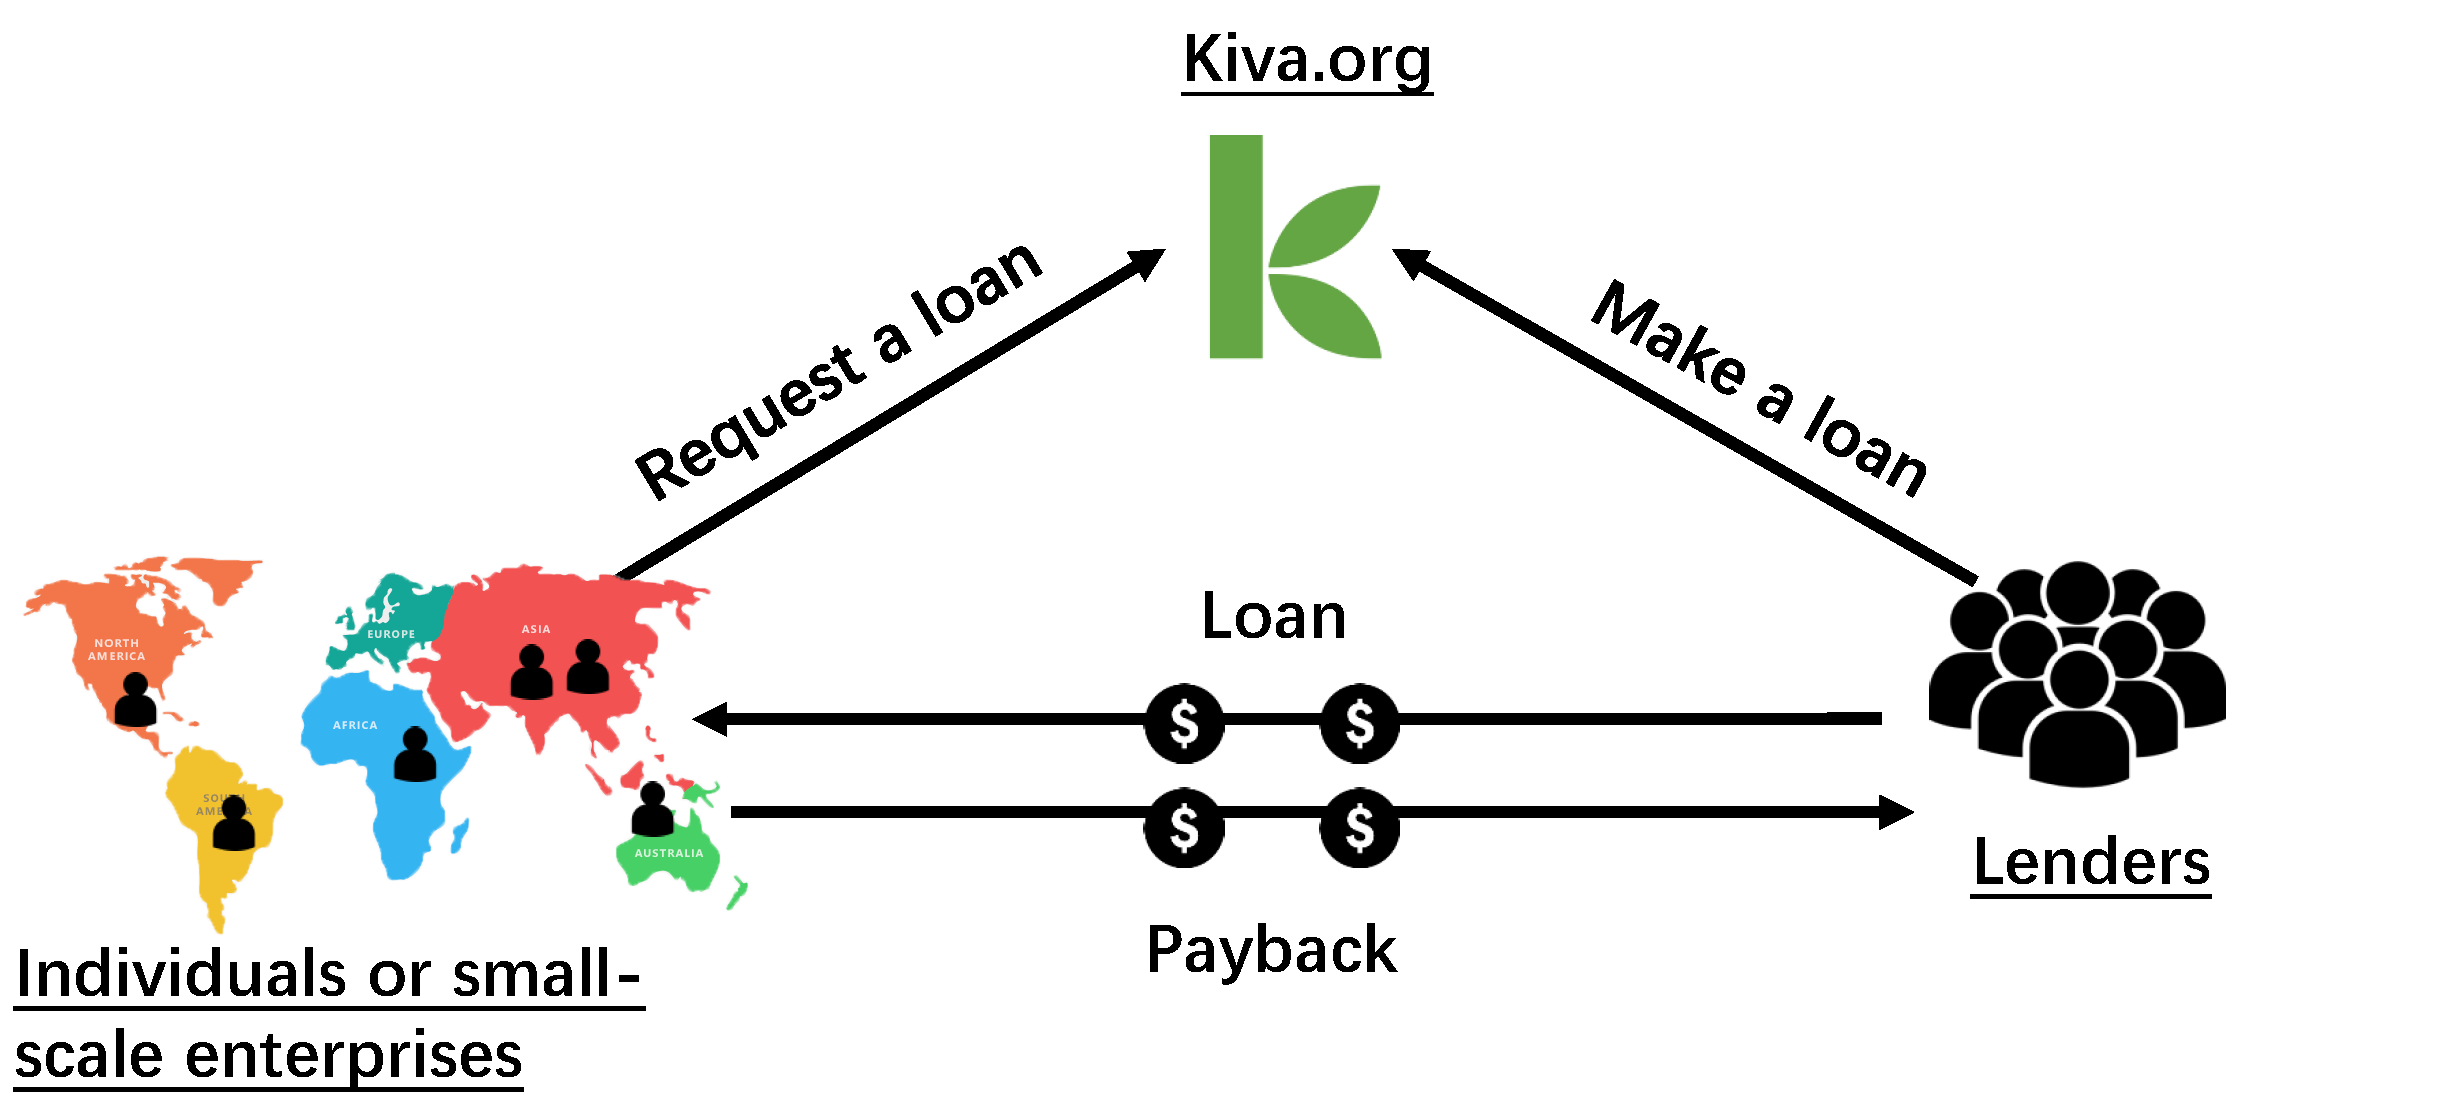
\includegraphics[width=0.98\columnwidth]{imgs/far/microlending.png}
        %\vspace{-0.25cm}
        \caption{Kiva.org provides an intermediary service for lenders and borrowers.}
        \label{fig:kiva_process}
        \end{figure}
        
        
        One key provider-side concern arising from Kiva's mission of supporting worldwide access to capital is that the geographic imbalances in users' preferences may manifest themselves in the disproportionate representation of certain countries or regions in recommendation lists. This could give rise to a positive feedback loop, as the recommended items are more likely to be supported, and thus the lending becomes even more highly concentrated. A similar kind of imbalance may arise with respect to different industries or economic sectors. Thus, we can identify at least two fairness concerns within this recommender system: equity in geographic distribution of capital \cite{liu2019personalized}, and equity across economic sectors \cite{sonboli2020opportunistic} which will be explained in detail in Chapter \ref{ch:fairness_postproc}. Other provider-side fairness concerns might arise in this context, e.g., the loan amount (loans with higher amounts get funded more slowly), but these are outside the scope of this thesis.
        
        % \todo[inline]{move this earlier}
        We situate our research within the organizational context of Kiva Microloans. This is a compelling case study to explore recommendation fairness since its fairness requirements are driven by internal needs surrounding its philanthropic mission, rather than external demands such as regulatory requirements found in financial services or employment, etc. A regulatory environment is more likely to provoke a defensive response related to fairness questions, which tends to hamper robust discussion of fairness properties in existing systems~\cite{chen2018fair,holstein2019improving}. A real-world example of Kiva's fairness-aware recommendations is depicted in Figure \ref{fig:kiva_underbanked}.
        
        
        \begin{figure}[htb]
        %\vspace{-0.25cm}
        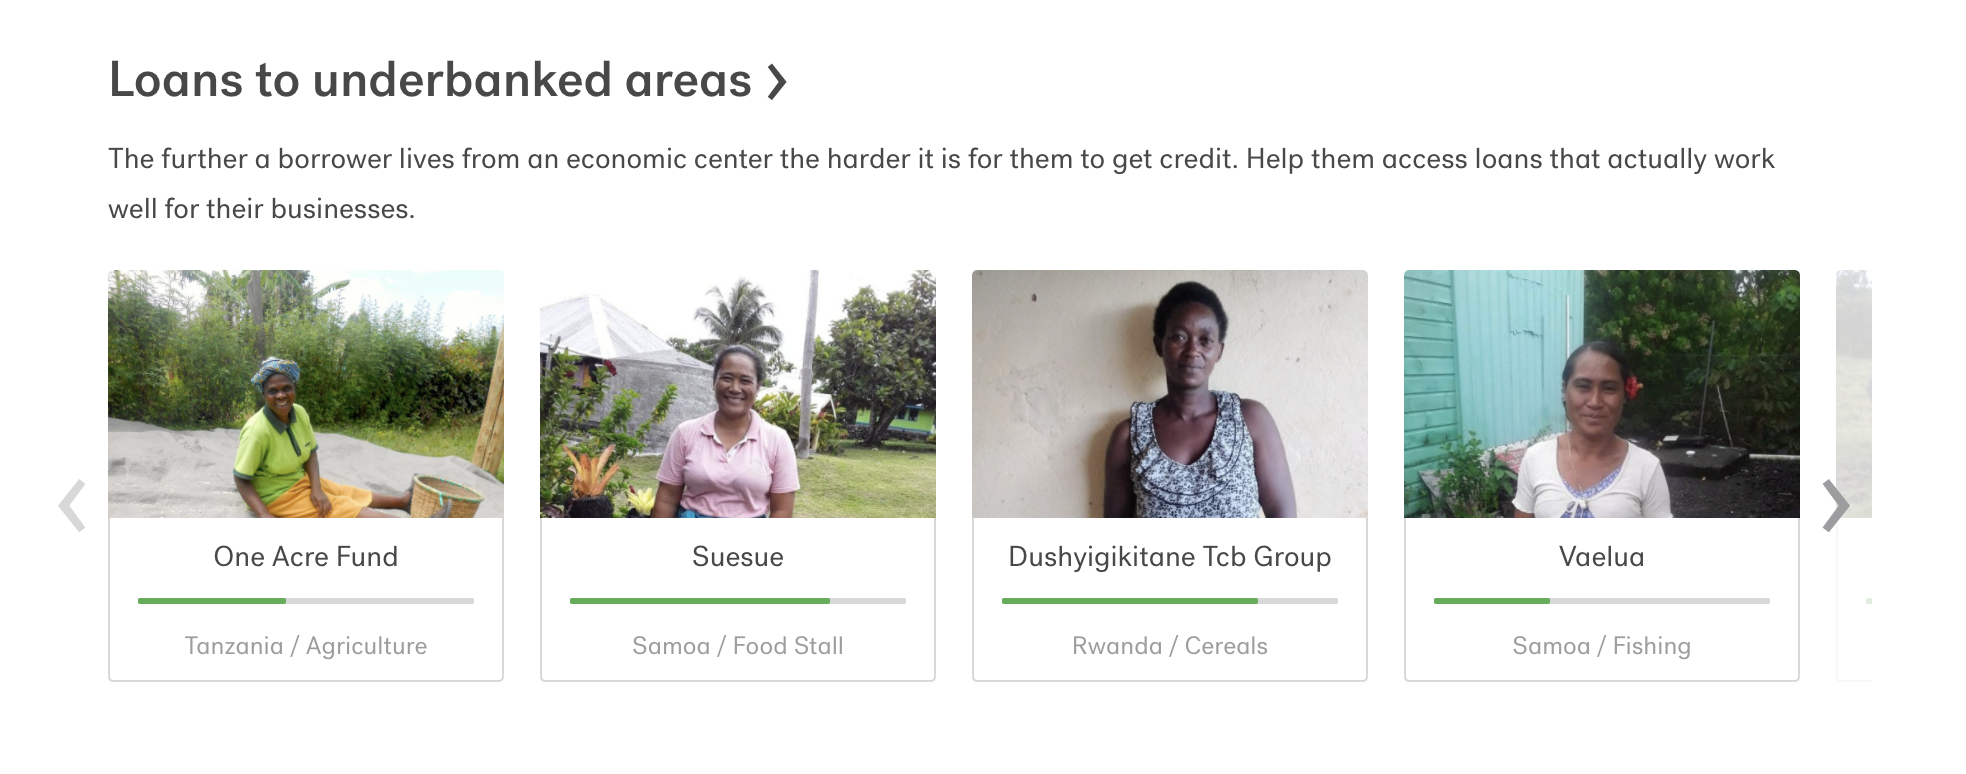
\includegraphics[width=0.98\columnwidth]{imgs/far/underbanked_areas.png}
        %\vspace{-0.25cm}
        \caption{Kiva.org provides fairness-aware recommendations.}
        \label{fig:kiva_underbanked}
        \end{figure}
        
        In addition, because of its philanthropic mission, it is reasonable to expect that Kiva's users will be receptive to fairness-oriented interventions. Finally, as a hybrid organization, embodying the characteristics of a nonprofit with the characteristics of a financial services institution, research embedded with Kiva is well-situated to have a broader and more generalizable impact across genres of institutions and sectors.
    
        % Loan recommendation, as in the case of Kiva is a suitable candidate for the exploration of recommendation fairness due to several reasons. One of them is that fairness requirements are driven by the internal needs surrounding Kiva's philanthropic mission to provide equitable access to capital for its borrowers regardless of their demographic information such as gender, the country of origin, etc., as well as other characteristics e.g. the economic sector for which they need the loan. Another reason reason on the suitability of Kiva is as follows: Kiva's users will be more receptive of the fairness-oriented interventions in recommendations due to its philanthropic nature whereas the users of a movie streaming website such as Netflix, might not care to be fair to the movie producers.
    

    \subsection{Streaming Media/E-commerce - Movie Recommendation}

        Streaming services for digital media consumption provide users with on-demand access to global content, connecting users with content creators, e.g., users and moviemakers on video streaming platforms like Netflix. Algorithmically generated recommendations power and shape the bulk of consumption patterns on such platforms. As Mehrotra et al. \cite{Mehrotra2018Towards} note, to maximize user satisfaction, streaming platforms that are optimizing for relevance could inadvertently be detrimental to exposure of the providers or content creators such as movie producers on the tail-end of the spectrum. As we have explained in the problem statement, optimizing only for relevance may lead to provider-unfairness, and consumer-unfairness.
        
        Therefore, streaming platforms carefully consider the influence of their recommendations on consumption patterns benefiting not only the users, but also creators, and the long-term goals of the platform itself. To better navigate such trade-offs between different stakeholder objectives, platforms are increasingly relying on multi-objective methods to jointly optimize multiple user-centric goals (e.g., engagement metrics like clicks, number of songs played, time spent), provider-centric goals (e.g., exposure) and platform-centric goals (e.g., fairness, discovery, diversity) \cite{mehrotra2020bandit}. In certain cases, aptly balancing such varied objectives makes it possible to obtain gains in both complementary and competing objectives.
        
        In this dissertation, we chose the movie recommendation context due to several reasons. Similar to the case of Kiva, fairness concerns regarding the exposure of the providers arise in these systems as well. We have addressed this issue in Chapter \ref{ch:fairness_postproc} in \cite{sonboli2020opportunistic,liu2019farpfar}.
        
        % \todo[inline]{cite dynamic fairness project}.
        
        Movie recommendation might not be an obvious candidate for the study of consumer-side fairness in recommender systems. Still, we used an approach similar to the method discussed by Yao, Sirui and Huang, Bert (2017) in \cite{yao2017beyond} to construct an artificial equity scenario within both MovieLens-1M and The Movies data for expository purposes only, with the understanding that real scenarios can be approached with a similar method. We chose MovieLens datasets due to the other following reasons: (a) MovieLens-1M is among the very few datasets with demographic information which makes it suitable for the use case of consumer-side fairness, (b) MovieLens-1M is a standard and commonly used dataset in the field of recommendation systems, and (c) generally, there is a lack of datasets in domains where fairness matters.


\section{Fairness Interventions in Recommendation Models}

    Fairness is a complex concept. It can have many different definitions under different contexts. More details on these concepts will be provided in Chapter \ref{ch:fairness}. In general, a system may have multiple \textit{fairness concerns}, particular aspects of its impact that may produce or perpetuate unfairness relative to a particular group measured in a specific way. This work concentrates on group fairness, focusing on increasing group fairness for under-privileged providers or consumers. %In other words, I intend to increase their exposure opportunities.
    
    % \todo[inline]{this term is not defined (fairness concerns)}
    After identifying the fairness concerns and defining them according to the context and application in use, it becomes possible to consider interventions in recommender systems to improve their fairness and performance. In doing so, it is worth keeping in mind the ``traps'' identified by Selbst et al. (2019) in \cite{selbst2019fairness}, possible hazards in applying fairness concepts in sociotechnical systems. Selbst and colleagues note that sometimes a technical fix is not always the most appropriate approach for problems of power imbalance and bias, and the failure to recognize this is defined as the \textit{solutionism trap}. There may be a wide variety of non-computational solutions to problems that surface themselves as unfair recommendations. Generally, three types of solutions have been proposed to operationalize fairness notions to mitigate unfairness: pre-processing, in-processing, and post-processing approaches.
    
    \textbf{Pre-processing} methods focus on compensating for the existing biases in a dataset, using different data collection enhancements to compensate for the biases that occur due to data imbalance. \textit{In-processing} approaches try to improve the fairness of results by integrating fairness notions into recommendation generation itself. \textit{Post-processing} approaches focus on modifying the outputs of algorithms to satisfy a fairness criterion. More details on these methods can be found in Chapter \ref{ch:fairness}. We propose one in-processing, and three post-processing approaches to improve the fairness-accuracy trade-off. Additionally, I will discuss the preliminary studies on a pre-processing method. More details are presented in Chapter \ref{ch:fairness_inproc}, and Chapter \ref{ch:fairness_postproc}. 
    % We run our experiments and analyze our results in the e-commerce and philanthropic contexts, which are explained in Chapter \ref{ch:methodology}.

%TODO check capital Chapter

% Throughout this dissertation, we propose different approaches to address achieving a better trade-off between accuracy and fairness. 

% For example, Kiva is a non-profit organization that operates a crowd-sourced microlending platform with the goal of financial global inclusion. In Kiva, the sides of the interaction are the borrowers, generally developing-world entrepreneurs who seek small amounts of capital to enhance their business capacity, and lenders, who are the application's end-users. A typical lender will contribute only a fraction of the total amount for any one loan, but may support multiple loans at any one time. Lenders do not get any interest on their investments and so supporting a Kiva borrower is essentially a philanthropic act. Kiva's mission emphasizes equitable access to capital for its borrowers, who generally cannot make use of traditional forms of banking and lending~\cite{choo2014gather}. Lenders are the users of the recommender system, which has the purpose of lowering their search costs in finding borrowers whose goals and needs appeal to them. 

% explaining the fairness issues
% Several provider-side fairness concerns might arise in this recommendation context.\footnote{Consumer-side fairness has not arisen so far as a concern in this application.} One key concern, arising from Kiva's mission of supporting world-wide access to capital, is that the geographic imbalances in users' preferences may manifest themselves in the disproportionate representation of certain countries or regions in recommendation lists. This could give rise to a positive feedback loop, as the recommended items are more likely to be supported, and thus the lending becomes even more highly concentrated. A similar kind of imbalance may arise with respect to different industries or economic sectors. Thus, we can identify at least two fairness concerns within this recommender system: equity in geographic distribution of capital \cite{liu2019personalized}, and equity across economic sectors \cite{sonboli2020opportunistic}.


\section{Research Questions}

%incomplete.. question and brief solution and the problems that it follows
The research questions that I seek to answer are as follows:
%TODO check I versus passive
\begin{itemize}
    \item (RQ1): How can we characterize the fairness/accuracy trade-off in different algorithms?
    % \todo[inline]{how does different algorithms compare (all rerankers), which algorithm should I use?}
    \item (RQ2): How can we incorporate fairness objectives into recommendation generation or post-processing to achieve better trade-offs? % far/pfar, ofair
    \item (RQ3): How can we extend these ideas to more complex scenarios involving multiple fairness concerns or requiring dynamic assessment of fairness opportunities? %dynamic fairness, multiple fairness concerns
    \item (RQ4): How can we ensure the reproducibility of the results and widen availability of fairness-aware techniques in recommender systems research? %librec
\end{itemize}


\section{Summary of Contributions}

My work here has primarily focused on developing recommendation approaches in which fairness metrics are jointly optimized along with recommendation accuracy. I have structured the problems and solutions to control and set the balance between accuracy and fairness. In other words, my goal is to improve group fairness while preserving accuracy as much as possible. Throughout the following work, I recognize all the stakeholders in a recommendation setting and propose solutions to improve fairness. I have used both error-based and exposure-based fairness metrics to assess unfairness of the results. 

I present the following contributions to the fairness-aware recommendation field. The first two contributions examine the first and second research questions. The third and fourth contributions investigate the third research question, and my contributions to the last project respond to the fourth research question.

\begin{itemize}
    \item \textbf{(Chapter \ref{ch:fairness_inproc}) Balanced Neighborhoods}:
    Here, I present an in-processing method to improve fairness while preserving as much accuracy as possible. Through introducing a regularization factor in the model, we provide a diverse neighborhood for each user. Diversity in every user's neighborhood ensures a less biased set of recommendations. Additionally, in his method, we can control the balance between fairness and accuracy via a hyper-parameter. Further, I define the concept of multi-sided fairness and demonstrate improvements in fairness for two sides of the recommendation setting: consumers and providers.
    % For more details please refer to Chapter \ref{ch:fairness_inproc}.
    
    \item \textbf{(Chapter \ref{ch:fairness_postproc}, Section \ref{sec:farpfar}) Fairness-Aware Recommendation Re-ranking (FAR) and Rersonalized Rairness-Aware Re-ranking (PFAR)}: 
    I describe two greedy re-ranking approaches here, both based on XQuAD (a method proposed by Santos et al. (2015)~\cite{santos2015search}, to increase diversity in lists for ranking methods). Both re-rankers are designed to increase group-based provider-side fairness and improve the fairness/accuracy trade-off. The developed methods here are purposed for a loan recommendation scenario, although they can be adapted to other contexts. 
    % This method is explained in details in Chapter \ref{ch:fairness_postproc}.
    
    \item \textbf{(Chapter \ref{ch:fairness_postproc}, Section \ref{sec:ofair}) Opportunistic Fairness-Aware Re-ranking (OFAiR)}:
    Here, I introduce the concept of opportunistic fairness. A novel method to improve personalization and fairness according to users' propensity to diversity in their recommendation lists. Additionally, I use a greedy re-ranking approach based on Maximal Marginal Relevance or MMR (a method presented by Xia et al. (2015)~\cite{xia2015learning} in the information retrieval field) to improve the accuracy/fairness trade-off for multiple aspects of fairness at the same time. 
    % This method is explained in details in Chapter \ref{ch:fairness_postproc}.

    % This post-processing approach is one of the few approaches that defines multi-aspect fairness and designs a method to improve different fairness goals of various providers in a simultaneous way. As an example, improving the visibility of impoverished loan borrowers with respect to different aspects such as: region of the world, their demographic information, loan amount, the economic sector, etc.
    
    % Users are not willing to experience diversity in every aspect of their recommendation. We detect the areas in which the users show willingness to see diversity and we consider them as opportunities to increase fairness without sacrificing much accuracy.
    
    \item \textbf{(Chapter \ref{ch:fairness_postproc}, Section \ref{sec:dynamicfair}) Social Choice for Re-ranking Under Fairness}:
    Here, I propose a novel framework for recommender systems called \textit{Social Choice for Re-ranking Under Fairness} (SCRUF). This framework is appropriate for dynamic environments where multiple fairness concerns matter. In this method, we use group-based exposure-based provider-side fairness definitions. 
    
    % This method is explained in details in Chapter \ref{ch:fairness_postproc}.
    %TODO make the title cases for all items consistent
    
    \item \textbf{(Chapter \ref{ch:librec-auto}) Standardizing and automating recommendation experiments via Librec-auto}: 
    Here, I present my contributions to \libauto{}, an open-source Python package incorporating different recommendation algorithms and evaluation methodologies. I have used \libauto{} throughout my dissertation to run experiments. 
    
    % For more details, please refer to Chapter \ref{ch:librec-auto}.
    
\end{itemize}



% 1) Can we maintain a high level of accuracy for the user base while increasing provider fairness? Or consumer fairness?

% 2) How can we control the accuracy trade-off better for providers? How to preserve accuracy while doing that? 

% 3) How can we control the accuracy fairness trade-off better for providers when addressing multiple fairness concerns? And can we use user propensities towards different categories to preserve accuracy as much as possible?

% 4) how can we achieve this balance dynamically?

% 5) What if we have data constraints? data minimization
% 6) Who controls the trade-off between accuracy and fairness? Should users have some agency over it? Should it be transparent to the users? Will re-rankers provide more transparency?


%%%%% incomplete


% This trade-off can have different underlying reasons. firstly, accuracy/personalization is a consumer-centric goal most of the time, and for example provider-side fairness is provider side. due to popularity bias, increasing personalization, might lead to less diversity for providers. and eventually less diversity for the consumers themselves. Achieving different goals at the same time might not be even possible. one other reason is the multi-party settings that recommendations offer, every one is striving to achieve what's best for them, and these goals might be competing. providers want one thing, the consumers want another thing. Therefore it's important to design methods to find a balance between these goals.


% \todo{mentioning that the cost of the data and EU rules, doesn't always allow up to gather more data, we do the data minimization then...}
% \todo{Do we need a summary of Contributions?}
% \todo[inline]{Do we need future work section?}



\singlespacing \chapter{Literature Review} \label{ch:lit}
\doublespacing This chapter covers literature that is relevant to the dissertation as a whole, and will frame each study's contributions broadly in order to synthesize across empirical work in \autoref{ch:synth}. Each individual study chapter (\autoref{ch:dbd} through \autoref{ch:wkshp}) includes a more specific literature review customized for each study.

\section{Complexities of Data Work in Nonprofit Organizations}
Research on data use within nonprofit organizations explains that diverse stakeholders (i.e. experts, volunteers, funders) complicate, but also facilitate data analysis, given a lack of expertise or capacity in-house, introducing complicated power dynamics along the way \citep{Voida2011Homebrew, Erete2016Storytelling, LeDantec2010Boundaries, Voida2017Currencies, Verma2016DrillDown}. Other research has shown that data often does not accurately represent an organization’s work in terms of format or content \citep{Verma2016DrillDown, Benjamin2012FrontOut, Benjamin2015Agency, Marshall2016Accountable}. This may at least partially be caused by the practice of more often using data for accountability purposes—mostly reporting to funders—than for making day-to-day operational decisions \citep{LeDantec2008Trenches, LeDantec2010Boundaries, Stoll2010Interorg, Voida2017Currencies}.

The dual use of data for accountability and operations has caused some organizations to perform double (or more) data entry—entering data once into a system for accountability purposes, while entering data into another system for operational use \citep{LeDantec2008Trenches}. Expertise around information technology and database technology capabilities varies greatly among organizations \citep{LeDantec2008Trenches, Stoll2010Interorg, Benjamin2018Policy}. When expertise around database technology falls short of organizational need, which is often the case, staff and volunteers often adapt what technology they have to partially meet their needs, resulting in hybrid locally-appropriated systems \citep{Voida2011Homebrew, Verma2016DrillDown, Stoll2010Interorg, Voida2017Currencies}.

Despite the challenges discussed so far, nonprofit staff sometimes do use data for decision making, however, the often rigid tools they have at their disposal are often not flexible enough to capture the clients’---and in fact the nonprofit’s own---circumstances. \citet{Harmon2017Fictions} determined that these IT systems place unrealistic expectations about how social good is accomplished, how effective programs can be, and to whom organizations should be accountable.

Where human service organizations are collecting data to make decisions, staff may use digital or paper forms as decision support tools to ensure decisions are made in the same way across staff and are based on evidence instead of a staff member’s intuition \citep{Schwalbe2004HS}. Despite this intended goal, \cite{Schwalbe2004HS}'s review of research on child welfare workers and mental health professionals found that their use of forms for making and recording decisions was inconsistent, and there was often disagreement among case managers. Research reviewed by \cite{Schwalbe2004HS} suggests that there at least three barriers to use of these decision support tools: (1) staff may intentionally modify data entered into the tool so that it outputs a decision that matches their assessment of the situation, (2) the underlying logic of the tool may be questioned, and (3) tools are dismissed in favor of qualitative accounts by staff.

The phenomena of ill-fitting data schemas, however, is hardly unique to human services (see \cite{Bowker2000Sorting} for an example of inconsistencies among doctors coding causes of death). Looking beyond client-level decision support tools, \cite{Benjamin2012FrontOut} found that common outcome measurement guides provided to nonprofit organizations advocate for metrics that align with the way that a program was designed to work, not the way it actually works in day-to-day practice. Therefore, when it comes to making both client-level and programmatic-level decisions, the data used within decision frameworks fall short of connecting on-the-ground program reality with representations of the local lived experience.

The social issues in which organizations intervene are complex. What it means to “do good” can be ambiguous and multiply interpreted, and as \cite{Voida2014SharedValues} showed, this multiple interpretability precipitates challenges when a particular logic of “doing good” is codified in one way in an information system, and that logic is inconsistent with the logic employed by social service workers. The “logics of the system” \citep{Voida2014SharedValues} are codified in extensions of the human services information system through decision support forms or a social program’s logic model---a formal document that outlines the way that a program intends to change something about society. \cite{Voida2014SharedValues} observe that while both the system and the implementers have shared values, such as increasing access to services for clients, “mismatches in the way values are understood and put into practice can create significant tensions.”

\section{Data Doubles and their Performativity}
Haggerty and Ericson introduced the construct of a “data double” as the digital profile of an individual that can be “transported to centralized locations to be reassembled and combined in ways that serve institutional agendas” \citep{Haggerty2006New}. Writing about the role of surveillance in society, Haggerty and Ericson observe that surveillance technologies do not monitor people as a comprehensive and static set of data points, but rather as a series of information flows, which they point out are subject to “pre-established classificatory criteria” \citep{Haggerty2006New}. 

\cite{Raley2013Dataveillance} expands on the data double concept by applying it to internet browser activity, pointing out that cookies allow advertising companies to assemble streams of data that are comprised of “flecks of identity” \citep{Fuller2005Media} to develop data doubles that could be used to personalize the targeting of ads. In the construction of a data double to represent the human being “[d]ata is in this respect performative: the composition of flecks and bits of data into a profile of [the individual], the re-grounding of abstract data in the targeting of an actual life, will have the effect of producing that life, that body, as [the profile]” \citep{Raley2013Dataveillance}.

The performativity of data has been studied in other contexts beyond the internet, such as rivers \citep{Ribes2013DataBite}, flora and fauna \citep{Bowker2000Bio}, medical metrics \citep{Pine2015Politics}, and food \citep{Voida2017Currencies}. \cite{Bowker2000Bio} observed that “what is not classified gets rendered invisible,” and items that are less charismatic are often not classified and therefore rendered invisible. For example, \cite{Bowker2000Sorting} argue that tropical diseases have largely been rendered invisible because they have not been included in the coding system used across the medical domain. As databases are structured around medical codes that exclude tropical diseases, the scientific data-driven world where these diseases are not acknowledged come to be “ever more readily recognized as ‘the real world’...” \citep{Bowker2000Bio}.

Within the nonprofit domain, \cite{Voida2017Currencies} argue that the database systems used by organizations and tuned to collecting particular data based on external stakeholder needs become performative by shaping “the future of the organizations and institutions that we rely on to promote the public good and remedy social injustice.” 

\section{Rational and Formal Logics}
The driving force behind the scientific charity movement---a systematized approach to social issues that began in the early 1900’s---stemmed from a desire to have large-scale social impact through scientifically backed top-down social engineering \citep{Sealander2003Curing}. The movement was particularly effective at influencing medicine and education, for example, in encouraging the adoption of corporate accounting and its associated logic of systematization \citep{Sealander2003Curing}. To support this approach, foundations that advocated for scientific charity encouraged higher education to grow (at that time) the relatively new area of social science to establish methods and metrics for deconstructing and studying all components of society \citep{Sealander2003Curing}. At the same time that the scientific charity movement was gaining momentum, this systematized approach also touched the business and government sectors. In the business world, it was through the scientific management movement, and in the government, it was through the creation of institutions like New York City's Bureau of Efficiency \citep{Brest2020Outcomes}.

A few decades later, the 1950’s and 1960’s saw the rise of the “high modernist” form of modernity, which encapsulates the belief in “supreme self-confidence about continued linear progress” \citep{Scott1998Seeing} through science and technology. This approach to progress is achieved through the application of scientific knowledge to “the rational design of social order, the growing satisfaction of human needs, and, not least, an increasing control over nature (including human nature) commensurate with scientific understanding of natural laws” \citep{Scott1998Seeing}. Not very far off in the distance, outcome measurement in nonprofit organizations as we understand it today---the process of recording and tracking an organization’s progress against their stated mission---began ramping up in the 1990’s in response to funder requirements \citep{Benjamin2012FrontOut,Brest2020Outcomes}. These funder requirements were shaped by over a century of a growing emphasis on evaluation by foundations like the Rockefeller Foundation and the Ford Foundation, which coincided with a similar emphasis in other sectors of society such as business and government \citep{Brest2020Outcomes}.

Today, the philanthropic movement called ‘effective altruism’ argues that “high-quality evidence and careful reasoning” are necessary in the social sector, and that “many people can...have a tremendous positive impact on the world, if they choose [social interventions] wisely” \citep{EffectiveAltruismIntro}. However, effective altruists are only a small portion of donors. Speaking more broadly, philanthropic research indicates that many foundations are “optimistic about evolutionary social change occurring through rational planning by so-called ‘politically neutral’ experts” \citep{Arnove2007Revisiting}.

This rational and evidence-based momentum plays out within nonprofit organizations as a strong push to evaluate their impact, which is often imagined by nonprofit employees as being possible through standardized quantitative metrics, whereas these employees believe that qualitative data only helps people “connect” with individual’s stories \citep{Verma2016DrillDown}.

This rational and scientific approach to work is viewed by \cite{Berg1997OfForms} as limiting the human element needed to do the work, explaining that “formal tools inevitably function in a rigid, impoverished way, thus de-skilling and dehumanizing the work of those who are caught in its cold, instrumental rationality.” Though, as \cite{Bowker2000Sorting} point out: “People do not really follow formal rules; they make up their own. They tailor rigid computer systems to their everyday working needs.” While the US nonprofit sector has a much longer history that predates the founding of the nation (see \citet{Hall2006History}), in summarizing its history starting in the early 1900's---as described above--- the nonprofit sector is deeply rooted in historical contexts that encourage social progress through rational and evidence-based approaches, though there are questions as to whether such an approach is well suited for socially impactful work.

\section{Map and Terrain}
The relationship between the representation of the local experience and its aggregate is a theme that weaves through numerous lines of work. Early studies of the French census, for example, highlighted that “no single set of categories could be adequate” and instead asked the local census authorities to supplement the national census categories with locally defined categories \citep{Porter1995Trust}.

The invention of scientific forestry in late eighteenth-century Prussia and Saxony developed the differentiation between---quite literally---the forest and the trees. These local and more global orientations connected to early modern European state efforts in aggregating the local terrain in the form of cadastral maps which would allow for easier management (and taxation) of territories without requiring intimate local knowledge. Conceptually, maps or aggregations of a geographic area are valued for their “abstraction and universality...[and] are designed to make the local situation legible to an outsider” \citep{Scott1998Seeing}. These maps, as Scott argues, present a simplified view “far more static and schematic than the actual social phenomena they presume to typify.”

Naive formalists believe that the map captures all the essential elements to base decision-making on, while opponents of that view express concerns about the level of interpretation and loss of detail in mapping the territory \citep{Berg1997OfForms}. However, the way people really use these tools falls somewhere between the two perspectives.

Just as decision-making occurs across both levels, the connection between the two worldviews remains extremely strong. The entity that is able to more seamlessly move between both worldviews is the data double, which can be examined as both a tree and, after aggregation, as a forest. This is only possible when a link is maintained between both levels. For example, in looking at water samples that are collected from local streams and analyzed to derive a number of metrics which can then be entered into a database, \cite{Ribes2013DataBite} point out that the stream’s data double relies on the linking back to the physical, local stream.

While the stream’s local identification number that maintains this link is simple and mundane (procedural metadata), if the ID becomes detached from the data double, the entire system breaks down because the sample cannot be associated with the source stream—in fact, relational databases work the same way. Connecting this observation more directly to the map/terrain metaphor, we can see the way that the terrain remains linked, yet becomes abstracted through the division of land west of the Ohio River into squares as influenced by Enlightenment rationalism. Regardless of the local terrain at those boundaries, the terrain is made legible at the map level thereby allowing it to be “registered and titled from a distance by someone who possessed virtually no local knowledge” \citep{Scott1998Seeing}.

The legibility of a local context at the map level opens it up to intrusion from outsiders, allowing them to navigate the terrain without the input of insiders, thereby reducing the privilege of local citizen’s knowledge \citep{Scott1998Seeing}. This form of surveillance that is possible at all levels, based on data doubles, is only possible “...provided a set of different databases are networked and provided that they share the same means of establishing individual identification” \citep{Raley2013Dataveillance}. 

Just as decisions about land management are made at the terrain and map levels, human services stakeholders also make decisions at the individual and aggregate levels. Within the literature on nonprofit data usage, \cite{LeDantec2008Trenches} break down the public sector into various “scales of influence and accountability” (referred to here as levels) that include local service providers, municipal entities, state, and national levels. They explain that “there are three characteristics that make scale crossing endemic in the public sector: upward accountability, lateral cooperation, and internal work practice.” Upward accountability includes lower levels reporting up to government, regulatory, and funding agencies; while lateral cooperation involves working with other organizations to provide a community service. “Finally, internal work practice comes to bear as the same information systems used to collect data (for upward accountabilities) and coordinate care (for lateral cooperation) are intended to support day-to-day case management” \citep{LeDantec2008Trenches}.

While the abstraction of local context for manipulation by higher levels of government and policymakers appears potentially problematic for the individual clients and citizens living within that local context, \cite{Raley2013Dataveillance} points out that “happily, sheer impracticality means that data systems can never function as perfectly as our dystopian imaginations might suspect. The errors inherent within a catalog mailing list, one of the more basic data sets, indicates how unstable that data can be: any given population is a massive moving target...”

\cite{Scott1998Seeing} also explains there are drawbacks to both local and global perspectives in that reality cannot be fully grasped at either level. The person on the ground cannot understand a city’s overall design as well as someone in a helicopter can, however the person up in the air also cannot understand the details of the street corner experience. \cite{Berg1997OfForms} argues that the formal and informal, map and terrain, do not exist as binary options, instead power is realized in the “interrelation” of the formal and informal. Additionally, \cite{Bowker2000Bio} points out that while a single database might be theoretically possible, many fields including medicine, have been attempting to do this for many years and have thus far not succeeded. Given this, \cite{Bowker2000Bio} suggests that instead we should “...look at the machines that produce local orderings and alignments of datasets (oligopticons),” referring to \cite{Latour2005ANT}'s oligopticon that is meant to be the inverse of the panopticon, where instead of seeing all, the guard sees very little, “but what they see, they see it well” facilitating “sturdy but extremely narrow views of the (connected) whole.”

\singlespacing \chapter{Sociotechnical Ecosystem} \label{ch:dbd}
\doublespacing \section{Preface}
This chapter was published in the Proceedings of the ACM Conference on Human Factors in Computing Systems in May 2017. It was titled ``Disempowered by Data:  Nonprofits, Social Enterprises,and the Consequences of Data-Driven Work'', and was co-authored with Ellie Harmon and Amy Voida (author order was Bopp, Harmon, Voida). It is included here as published with the permission of my co-authors.

\section{Introduction}
In the move toward rationalization and quantification in organizations \citep{Morgan1997Images}, the increasing prevalence of information systems designed to support the collection, management, and analysis of data has coincided with expectations that organizations should be more “data-driven”---using increasingly larger aggregations of data to enable more productive and empowered decisions. Previous research in the management of information systems has suggested that, in for-profit contexts, data-driven decision making leads to improvements in performance, output, and productivity \citep{Brynjolfsson2011Strength,Lavalle2011Big}. In the nonprofit context, data-driven decision making has been shown to improve “the effectiveness of management decisions” \citep{Maxwell2016Data} (see also \citep{Leroux2010Does}). Yet scholarship about data and its impacts on organizations in HCI and adjacent fields has raised critical concerns about this “march toward quantification” \citep{Lohr2012Age}---concerns about the ways in which the quantification of data changes assumptions about the meaning of knowledge and about how people “should” engage with information, concerns about the biases inherent in and the decontextualization of big data, and concerns about the new digital divides created by big data \citep{Boyd2012Critical,Pine2015Emerging,Punathambekar2015Debating}.

Recent empirical research has also raised significant concerns about how “cultures of data” are enacted in organizations \citep{Verma2016DrillDown}. This research has identified significant disconnects between the support provided by collaborative computing systems and the organizational practices that are developing in response to calls for organizations to become more data-driven. In addition, questions remain about how work practices and organizational identity are shaped by the expectations and demands of being data-driven \citep{Pine2015Emerging,Power1997Audit,Pentland2000Auditors}.

In this research, we expand on this nascent but growing body of empirical work by examining the enactment---and consequences---of monitoring and evaluation (M\&E) in mission-driven organizations. Encompassing nonprofit organizations and social enterprises, mission-driven organizations differ from traditional for-profit corporations in that organizational goals are rooted in social impact, rather than solely in profit-based bottom lines.

Research about the uptake of data-driven practices in the mission-driven context is critical as recent investigations have raised concerns over the efficacy of data practices in mission-driven organizations. Maxwell et al. found that in social enterprise organizations, “data are often collected but less often analyzed” \citep{Maxwell2016Data}. And although individuals in these organizations believed in the potential of data-driven decision making, they reported “less confidence in their organization’s ability to do so” \citep{Maxwell2016Data}. 

In this paper, we present findings from an empirical study of the use of data in 13 mission-driven organizations. Drawing on interviews with 19 M\&E professionals, we find critical consequences in how data practices are emerging in these organizations. The mission-driven organizations that participated in this research are not empowered by data. Instead, they are investing time, sacrificing expertise, and responding to largely external demands for data collection and reporting at the expense of the mission and operation of the organization. We identify three negative consequences of current data practices---\textit{erosion of autonomy, data drift, and data fragmentation}---which are mutually reinforcing and lead to a cycle of increasing disempowerment. This \textit{cycle of disempowerment} results in organizations having less control over their own data practices—preventing the meaningful use of data and discouraging the organization from redesigning data practices to better meet their needs.

\section{Related Work}
\subsection{Data-Driven Practices}

Researchers have identified many benefits of using technology for data-driven practices, including the optimization of production and manufacturing, reductions in customer attrition, reductions in data redundancy, facilitation of new genres of questions by end-users, increased profitability, and the creation of competitive advantage \citep{Kohavi2002Trends,Piccoli2008Profit,Watson2007Current}. When these tools are successfully leveraged for data-driven decision making, these practices are found to improve performance, productivity, and effectiveness \citep{Brynjolfsson2011Strength,Lavalle2011Big,Leroux2010Does}.

Yet, previous research has also raised concerns about the biases of big data leading to new digital divides between data-haves and have-nots and between individuals and organizations that do and do not have computational literacies \citep{Boyd2012Critical,Kitchin2014Big,Manovich2011Trending}. Manovich suggests that big data has created new inequalities among three categories of people and organizations: “those who create data (both consciously and by leaving digital footprints), those who have the means to collect it, and those who have expertise to analyze it.” \citep{Manovich2011Trending}

boyd and Crawford suggest that two digital divides fall out of these inequalities: one related to who does and does not have access to big data and a second related to who does and does not have the ability to \textit{utilize} this data \citep{Boyd2012Critical}. Concerns about the uneven uptake of big data become even more critical as the purview of data-driven practices are expanding beyond the private sector. As King asserts:

\begin{quote}\singlespacing The march of quantification, made possible by enormous new sources of data, will sweep through academia, business and government. There is no area that is going to be untouched (quoted in \citep{Lohr2012Age}; see also \citep{Brynjolfsson2011Boom,Kitchin2014Big}).\end{quote}

It becomes increasingly important, then, to understand the ways in which data-driven practices are taken up or attempted in a diversity of organizational contexts.

\subsection{Data in the Nonprofit Sector}
Nearly all research exploring the role of technology in the nonprofit sector highlights the extraordinary constraints in resources and expertise that shape the way systems are and are not used (e.g., \cite{Merkel2007Learning,Voida2011Homebrew}). Information management, in particular, is a challenge for these organizations. Voida et al. have characterized the patchwork assemblages of information systems in the nonprofit sector as “homebrew databases” \citep{Voida2011Homebrew}. Working within the myriad of constraints in these organizations, individual knowledge workers creatively appropriate disparate paper tools, personal information management systems, and---sometimes---enterprise or custom databases to satisfice their data practices. But these “homebrew databases” are plagued with significant version control issues, redundant data entry, a lack of scalability, siloed and/or inaccessible data, an unproductive churn through the adoption and use of different tools, and, ultimately, an abandonment of data. 

These challenges are not solved in even the leading edge organizations in the sector. Verma and Voida’s case study of one such organization’s adoption of a business intelligence system also found pervasive challenges in data warehousing \citep{Verma2016DrillDown}. Much of the organization’s data was siloed in systems for which there was no import mechanism; some data was kept in spreadsheets and had to be manually updated daily; and some data was not digitized at all. 

All of these issues make engaging in data analysis a nearly intractable problem. Perhaps it is unsurprising, then, that a survey of the capacity for data-driven decision making in social enterprise organizations found that while organizations are collecting a large quantity of data, they are not adept or confident about analyzing or using that data \citep{Maxwell2016Data}. 

Supporting information management in the nonprofit sector is particularly important as these organizations are under increasing pressure to provide impact and performance data to funders \citep{Haskins2011Building}. Yet, Snibbe warns of the costs: “Nonprofits are often collecting heaps of dubious data, at great cost to themselves and ultimately to the people they serve” \citep{Snibbe2006Drown}. Indeed, research in philanthropic studies cautions that many of the performance metrics used in nonprofit organizations fail to account for critical aspects of nonprofit work and, in fact, might be impeding performance \citep{Benjamin2014Programs}. Understanding the role of data in the work of mission-driven organizations will be critical to better supporting and empowering these organizations.

\section{Methods}
\subsection{Participants}

We recruited 19 participants (referenced by an anonymous participant number, P1–P19) from 13 mission-driven organizations, all of whom were responsible for some aspect of the monitoring and evaluation (M\&E) work in their organization. M\&E professionals typically serve as the central points of expertise regarding data in their organization, often responsible for operationalizing and carrying out requests for data—whether originating inside or outside the organization. As such, these individuals offer a uniquely broad perspective about how data is taken up and used---and the implications of that use---across the organization. We recruited participants initially through snowball sampling, starting with M\&E professionals who participated in a community professional development event. As our research unfolded, we engaged in theoretical sampling, strategically recruiting from additional organizations to obtain diversity on two dimensions: type of organization and annual revenue.

We sampled from three types of mission-driven organizations to create maximum variation:

\begin{enumerate}
\item Direct service nonprofit organizations provide a variety of services to clients (n=9 participants from 8 organizations);
\item Indirect service nonprofit organizations provide services to other nonprofit organizations, including research services and funding (n=9 participants from 4 organizations); and
\item Social enterprises are mission-driven, for-profit organizations or programs within nonprofit organizations (n=1 participant from 1 for-profit social enterprise, plus n=8 participants already included above from 6 nonprofit organizations who manage social enterprise programs).
\end{enumerate}

We also sampled across a range of organizations’ annual revenue. Because data practices are often prescribed by funders, we consider a range of annual revenues to signify a range of experiences with data practices. Organizations sampled ranged in annual revenue from \$100K to \$75M. Within these annual revenue figures we, once again, used available data to sample across predominant revenue sources: government grants, membership dues, fundraising events, program service revenue, and sale of inventory.

\subsection{Data Collection}
We collected data through semi-structured interviews using an interview protocol that focused on three areas of inquiry: (1) the nature of the participant’s work within and/or alongside other mission-driven organizations, (2) the role of data and related technologies in the participants’ work, and (3) the organizations’ approaches to impact measurement including the types of data collected and the information systems leveraged. The first author conducted all interviews and adapted the interview protocol based on grounded theory’s principle of constant comparison to gather “additional data samples that are chosen to test the theory at its weakest point” \citep{Muller2014Grounded}. One interview question, for example began broadly as ‘How and why do you collect data on your organization’s programs?’ and evolved into a request, for each type of data, for the participant to ‘tell [us] more about who the audience is and how that audience shaped the process.’ This evolution was driven by accounts of power and influence offered by early study participants and was designed to better understand how external audiences were or were not involved in the day-to-day operational decisions of data collection and at what level of specificity.

Interviews lasted on average 56 minutes. The majority of the interviews were conducted within a one month period, with additional interviews conducted several months later after preliminary data analysis. We audiotaped and transcribed each interview to aid in analysis.

\subsection{Data Analysis}
We took an inductive approach to data analysis (following \cite{Corbin2014Basics}), grounded in coding and memoing techniques. We identified emergent themes such as evaluative approaches, organizational constraints, and technical capacity through open coding. We printed, cut up, and clustered the coded transcripts to develop axial codes that surfaced themes about the relationship between organizations’ internal capacities, externally imposed constraints, and data complexity.

We interleaved the second stage of analysis with additional data collection, using our axial codes to “interrogate the open codes, leading to more data collection and more open coding” \citep{Muller2014Grounded}. We then engaged in several iterations of affinity diagramming to identify cross-cutting categories that allowed us to make sense of participants’ experiences and understandings of M\&E work in mission-driven organizations. We tested each at its weakest point through memos and discussions among researchers, frequently returning to the transcripts as reference. This multi-stage analytic process resulted in the identification of three key consequences of monitoring and evaluation. In subsequent theoretical integration, we explored the interrelationships among these consequences, leading us to propose a \textit{cycle of disempowerment} for mission-driven organizations.

\subsection{Methodological Limitations}
Grounded theory---and all research methods—include many trade---offs in the kinds of evidence they generate and the kinds of conclusions and theory building they facilitate. An interview-based grounded theory approach is well suited to this research as we sought to understand the practices, experiences, and implications of data in mission-driven organizations. This approach offers opportunities for what \cite{Lincoln1985Naturalistic} refer to as “transferability”---the evidence-based argument that analytical insights are applicable beyond the specific individuals studied. This affordance of qualitative methods is enabled by strategies such as constant comparison rather than being rooted in ideals of statistical generalizability or bias-free objectivity \citep{Lincoln1985Naturalistic}.

\subsection{Research Context: Monitoring \& Evaluation in Mission Driven Organizations}
Mission-driven organizations are entities, both large and small, for-profit and not-for-profit, that aim to have a particular impact on society as described by their organizational mission. Generally, this mission is geared toward having an effect on one or more critical issues facing society, such as health or education. For the purpose of this study, organizations were considered mission-driven if they were either a traditional nonprofit organization or a social enterprise that placed the importance of social impact at an equal or greater level than profit.

The hub of data collection and use within mission driven organizations is the monitoring and evaluation (M\&E) department or, more likely, a singular M\&E professional who may also have several other job responsibilities. The individual(s) responsible for M\&E oversee the on-going monitoring of program activities against targeted outputs and outcomes. They also may conduct more comprehensive retrospective evaluations that examine the program’s operation and assess progress towards intended short-term and long-term outcomes. This work often involves orienting to an organizational “theory of change,” a model that (a) represents how a social intervention intends to use resources to perform programmatic activities and ultimately achieve the desired social impact, and (b) suggests specific metrics that the organization should be using to measure impact.

The unique mission-driven context shapes organizations’ relationships to data, impacts how that data can ultimately be put to use, and influences to what ends and for whom it can serve. To situate the findings of this work, we first provide some background on four key characteristics of the mission-driven context: limited resources, grant-driven business models, social impact measurement, and reliance on external experts. Each characteristic is well-established in nonprofit management but where appropriate, we augment our characterization with specific references to participants in this study to illustrate more concretely how these characteristics influence data practices.

\subsubsection{Limited Resources}
The experiences of participants in this research confirm prior findings that nonprofits have limited financial and labor resources (e.g., \cite{Merkel2007Learning,Voida2011Homebrew}). These limitations influence data practices from collection to analysis to reporting. Participants were particularly attuned to the limitations of time as a resource, and framed many of their frustrations in terms of having to make difficult tradeoffs as a result. Often, organizations restrict the time spent on data practices to that which is obligated by external funders. So while significant time is devoted to collecting data, analyzing that data beyond the production of reports for external funders is rare.

\subsubsection{Grant-Driven Business Model}
The organizations in this research were all, to varying degrees, reliant on grants made by external funding agencies to carry out their work. This means that funders have significant sway over organizations, which we see manifesting through prescriptions about what data to collect, how to report on it and how to interpret it. Organizations with funding from multiple sources had to negotiate compounding—and sometimes conflicting—requirements for data collection, management, and reporting. This can be problematic because it amplifies an existing challenge that arises from a misalignment of goals between funding bodies and the organizations themselves.

\subsubsection{Social Impact Measurement}
Mission-driven organizations try to intervene in complex, large-scale social issues that make both data collection and analysis difficult. Any change caused by the work of the organization is intertwined with—and likely indistinguishable from—the variety of other social changes happening concurrently: ranging from changes in government programs, to local economic shifts, to even more localized changes within the lives of families and individuals served by organizations. Organizational “impact” is not easily disentangled or isolated in ways that may be attributed causally to a particular program. 

Complicating the difficulties of establishing causality, social impact is something that cannot be achieved overnight---it takes time. This means that data collection must be longitudinal in order to be most useful. Yet, knowing what data to collect at the start of a program is often impossible. Consequently, datasets collected by organizations are often incomplete---beginning with one set of metrics, and shifting over time to include more or simply different metrics. 

\subsubsection{Reliance on External Experts}
Similar to the findings of Erete et al that described nonprofits’ reliance on external experts for “open data” work \citep{Erete2016Storytelling}, we found that M\&E data practices are also generally reliant on external experts. For the organizations in this study, external experts included: professional evaluators, researchers, graduate student interns, data scientists, regional coordinators, and technology consultants. M\&E professionals have expectations about the differing abilities of each group, with volunteer data scientists providing “game changing” assistance and interns providing hit-or-miss help. Yet, in the case of smaller, more resource-constrained organizations, unpaid interns are the only realistic option. Organizations with more financial resources were more likely to have a dedicated “data analyst” on staff, however, even in these cases professional consultants are still hired on a temporary basis. Despite differing levels of knowledge and experience, our participants generally felt that all of these experts have the necessary expertise to be able to work with the intricacies of their data. 

\section{Findings}
We find that mission-driven organizations’ monitoring and evaluation (M\&E) practices result in three unforeseen and negative consequences that are mutually reinforcing and lead to a cycle of increasing disempowerment for the organization. These consequences are: \textit{erosion of autonomy, data drift, and data fragmentation}.

\subsection{Erosion of Autonomy}
All participants described experiencing an \textit{erosion of autonomy}---including individual and organizational autonomy---over data practices due to the influence of external actors, including funding bodies, boards, ratings agencies, and information technologies. This array of actors exerts influence, impinging upon organizations’ autonomy in making decisions about choosing metrics, compiling and using data, and prioritizing data work.

\subsubsection{Choosing Metrics}
Before decisions about data use could be made, participants’ accounts suggest that external actors wore away at organizations’ autonomy in making choices about what data should be collected and what metrics should be computed. P8, for example, described getting...

\begin{quote}\singlespacing...caught up in reporting the indicators that are required to the people that are paying the bills rather than necessarily taking space to step back and look at the whole picture. (P8)\end{quote}

Compounding long-standing requirements of funding bodies for certain data---e.g. beneficiary demographic data, or output metrics like number of people served---external groups are asking for additional, more specific, data. One participant described the recent actions of a rating agency: “They’re trying to have organizations fill out [forms to answer the question of] how do you know what you’re doing makes a difference?” (P3)

Though rating agencies have historically relied on data from tax forms, a participant who worked for a nonprofit organization that assigns ratings to other nonprofits affirmed that agencies are increasingly asking organizations to provide additional data, particularly impact data: “If you want to get your 4-star rating, you’re going to have to be talking about how you’re tracking impact” (P4). Similarly, another participant speaks about funders:

\begin{quote}\singlespacing 20 years ago, output data was really the only thing we had and that’s all people asked for, was, you know, how many people did you serve? Well now, for sophisticated funders, that’s not enough. (P14)\end{quote}

\subsubsection{Compiling and Using Data}
When it comes to making decisions about how to operationalize measures like impact, organizations in this study were not only pressured about what data to collect, but also about what \textit{kind} of data to use for what purpose. Board members wanted to market “feel good” (P12) stories informally obtained outside of the evaluation process:

\begin{quote}\singlespacing Our board...they get real hung up on the marketing story instead of, well, what's the evidence for the marketing story? I've introduced this phrase \textit{evidence-based marketing metrics} to them, but it's kind of a struggle. I would like this [evaluation] data to be used for board and fundraisers to be able to have some real things to report on instead of 'Oh, it's all so great!' (P12)\end{quote}

Board members further shaped organizations’ data practices through constraints about how data should be reported. In our participants’ experiences, board members are more interested in looking at executive summaries of data analysis---more conducive to glance-able graphs or a “feel good” quote, not details of nuanced analyses.

As organizations move towards computational systems of measurement, they are also encountering information systems that prioritize quantitative over qualitative forms of data. As P10 explained about her organization’s database: “We would need to have people answer qualitative questions in a quantitative way. So, ‘how did this make you feel on a scale of 1 to 10?’” (P10) 

Even at the funder level, information systems served to steer staff members towards quantitative data that can more easily be accessed and queried. This was explained by a staff member at a community foundation:

\begin{quote}\singlespacing Any reporting...[on] the difference we made in the community...is outside of any formal IT system. It’s coming in probably on a dozen different channels, with a dozen different formats and it’s not centralized. So, if someone were to say I need to measure our impact, [the IT systems] wouldn’t be very much help. [Using the database], I could tell them where the money went...[but] if you want to know the stories...about what difference we made, you need to go talk to [a program staff member] because I don’t have anything I can touch that gets to that. (P16)\end{quote}

In addition to these constraints on what data to collect and what kinds of data are considered valuable, participants’ accounts suggests that decisions about how to use data were further sites of eroded autonomy. There is a key distinction between the evaluation work required by funders and a more rigorous evaluation that would more closely benefit the mission of the organization. Often, evaluation work required by grants, referred to as “implementation evaluation” by P15, is not intended to understand how a program has caused a change in society, instead it is intended to determine if the grant dollars were spent in the agreed upon manner.

\begin{quote}\singlespacing Funders are interested in building evaluation in around the specific objectives of that project...It’s more of an implementation research question that funders have...Really rigorous evaluation of what works...that’s the type of evaluation that it’s harder to get a funder to say ‘Oh yeah, I’ll do that.’ For instance, we have a couple projects where...we have a comparison group that we’re working with that isn’t getting the intervention. That type of project is expensive, and funders have to have the vision to see that what we’ll learn from that might have a lot of later potential impact if we know if the intervention works. (P15)\end{quote}

When broader social impacts are valued, report preparation timelines can prohibit longer term evaluations as granting agencies operate on short-term cycles (and thereby encourage surface level evaluation) rather than asking for or rewarding in-depth and longitudinal evaluation. Moreover, participants reported challenges in putting reports to use internally which had been prepared for the primary consumption of external stakeholders. For P10, it is challenging to resist the option of “just taking the report and putting it on the shelf” (P10). Even though a report might contain potentially useful data about operations, leveraging the report in ways that might inform internal practices would require additional time that staff do not have. 

\subsubsection{Prioritizing Data Work}
The many data collection requirements and the use of data by external actors to evaluate and rate mission-driven organizations contribute to eroding organizations’ autonomy over their own processes. This occurs at the most mundane and micromanaging kind of level: how to prioritize staff time. Staff members in this study reported a lack of time to accomplish their many tasks which often resulted in a prioritization of data work for funders over that which might be done for the organization. One participant explained: “Taking all of that data, entering it into something that makes it make sense, and figuring out how to use it is never a priority when there are fires to put out every day” (P8). Despite these fires, P8 finds time to collect and report on indicators that the funders want.

The kinds of rigorous evaluations that participants report would allow organizations to examine their own programs in terms of long-term causal outcomes are not supported within the rubric of most grants, the data demands of ratings agencies, or the information systems designed for tracking and analyzing only limited kinds of metrics. Funding for additional data work is harder to find in the mission-driven environment, which is increasingly dominated by directed funding earmarked for specific programs. Initiatives to build organizational capacity and infrastructure for data work---often referred to as “administrative overhead”---weighs against an organization’s perceived effectiveness and efficiency in carrying out their mission.

When data collection must conform to frameworks and blueprints dictated by funders, organizations are left juggling everyone’s needs except their own. The accounts of data work reflected by participants suggests that organizations are operating within a cacophony of data strategies. Regardless of who is setting the direction and what their motivation is, choices about what data to collect and report are partially driven by whomever happens to be providing direction. In this diverse ecosystem of data stakeholders, it is unclear that there is ever a single, overarching plan. What is clear, however, is that the organizations, themselves, have relatively little autonomy in setting or even providing input into that overarching plan---which lays a foundation for organizational disempowerment.

\subsection{Data Drift}
The nonprofit sector refers to the move away from an organization’s mission over time as “mission drift” \citep{Moore2000Managing}. Mission drift has severely negative connotations as organizations are involuntarily and unknowingly pulled away from their original mission toward a new one. In our research, we see a similar shift at the level of data. Through \textit{data drift}, organizations change the kind of metrics that they collect and manage over time as their organizational identity, as represented by data, evolves. Despite the possibility that an approach to M\&E may not be a good match for the organization, an eroding autonomy can prevent them from putting their data trajectory back on course. As misguided data is used in evaluation and funding decisions, the next round of data collection requirements are likely to be even further from the organization’s intended direction.

For the participants in this study, external influences cause \textit{data drift} at multiple stages of the organization’s workflow: from initial, orienting theories of change to final reporting. For example, one participant (P11) described how the organization’s theory of change was developed not from rigorous research or impact measurement, but rather based on the \textit{funder’s} objectives by “scoping and identifying” where their project had the most demonstrable impact. In this instance, the funder was comparatively hands-off, yet still indirectly manipulated the way that staff viewed their program’s impact. Theories of change influence choices of what indicators to track, and defining change rooted in funders’ objectives leads to shifts in data collection towards the funder’s priorities, all the while neglecting metrics more squarely related to the organization’s own mission.

In another instance, one executive director (P8) explained that she sees her organization as helping individuals escape poverty. However, one of their two primary funders is particularly interested in their work in terms of its environmental impact---because that is the funder’s mission. From the nonprofit’s perspective, they feel that their program’s environmental impact is “nothing” compared to other renewable energy projects. However, the funder is “very interested in those environmental indicators, and so we end up doing a lot of weird environmental stuff that we don’t typically focus on” (P8). Thus, \textit{data drift} is perpetuated in this organization because of their ambivalence about pushing back on a “strong” funder. P8 continues by describing how funders shape data collection decisions:

\begin{quote}\singlespacing We find ourselves kind of hustling to do M\&E in a way that might not necessarily always make sense for us. But we need it for a report, and we need these numbers and even if it’s something that we’ve never thought about collecting before, it’s like, well, figure out how to collect it because so and so says we need it. (P8)\end{quote}

P8 goes on to describe how grant-based funding can impact the mission of the organization over time:

\begin{quote}\singlespacing [It is] not a very sustainable way to ensure effective sustainable growth... It’s really hard to find the perfect fit grant that allows you to just keep doing what it is that you know your organization does best. Because you then end up tied to... the indicators or the activities... as dictated by what your funder wants to see. (P8)\end{quote}

This reflection suggests that \textit{data drift} may function as a precursor to mission drift. As data is collected in accordance with the funder’s desires, the organization may shift focus, further contributing to organizational disempowerment.

\subsection{Data Fragmentation}

Compounding this situation of \textit{data drift}, funders struggle to determine what data they should require from organizations in the first place. This lack of clarity at the funder level, coupled with the fact that many organizations are juggling the demands of multiple funders---a complicated puzzle that organizations must negotiate with their limited resources---results in an accumulation of fragmented data sets. Numerous participants reported being plagued by a proliferation of data that were not connected to each other in any systematic way, creating difficulties for performing social impact measurement. The resulting fractured and incoherent set of data is hard to analyze or put to any kind of use. Thus, while participants reported “swimming in data” (P15), the lack of a systematic data plan from the organization’s point of view limits and constrains the usefulness and impact of data, leading to further organizational disempowerment. The \textit{data fragmentation} reported by participants is multi-faceted. It is fragmented locationally, logically, and longitudinally.

\subsubsection{Locational Fragmentation}
Locational fragmentation occurs when different data are in different systems. For two participants, locational fragmentation resulted from a lack of funding that prevented them from accessing a single, centralized enterprise-level data management system. Instead, in both of these cases, participants’ leveraged multiple, free cloud services for storing data. As P11 explained, data management is particularly difficult “across a team... who don’t have a lot of money to invest in cloud services besides Dropbox and Google” (P11).

Such cases of locational fragmentation were a frequent source of confusion (see also \citep{Voida2013Turbulence}) at another organization:

\begin{quote}\singlespacing [There is not] one place where we can have everything, it’s like OK well you have Google Drive, and some people use Dropbox and some people use our database... it’s really confusing to be like well where was that data stored?... [I received] an invitation for Dropbox stuff a couple days ago. It’s like ahh, I forgot we were using that for stuff, for some reason, I don’t know why we were—probably ran out of room on Google Drive so they started using something else. (P7)\end{quote}

In addition to this locational fragmentation that occurs within individual organizations, locational fragmentation also occurs across organizational boundaries. All participants in this research discussed sharing data with external parties and relying on others to share relevant data in return. Yet, this sharing of data across organizations was not always easy to negotiate and relied on both trust and equitable power dynamics. As P8, explained, there was a relevant dataset that existed within another organization. P8’s organization could not access it quite yet because they are waiting until they “have a slightly stronger relationship” (P8).

When one organization possessed some level of power over another organization, the exchange of data can be mandated, thereby mitigating locational fragmentation for the organization with power but contributing to a \textit{cycle of disempowerment} for the organization without it. The organization that P1 works for explains:

\begin{quote}\singlespacing We can’t really require them to do [any data entry]. The [participants in another program] are required because we’re actually providing them consultants for free. (P1)\end{quote}

\subsubsection{Logical Fragmentation}

Complicating the distributed data storage locations, data was also logically fragmented---data sets discussed by participants did not complement each another in a systematic way. This fragmentation was observed in disparate data sets whose motivations for collection were determined through isolated processes by unique individuals or groups.

One M\&E intern discussed the changes in organizational context that led to the logical fragmentation of their data:

\begin{quote}\singlespacing They had the head of the region... implementing just plain spreadsheets... I started redoing that entire thing... No one had really tackled that piece before. So, I think that they were suffering from kind of poor structure. And they were trying to grow. No one was thinking about putting systems in place from the start. (P9)\end{quote}

In a different organization, staff turnover led to difficulty integrating a new dataset with two previously existing datasets. At the time of the interview, the participant was looking for a graduate student intern to “see where the compatibilities are... [to] see if we could kind of merge these data sets so we have something to work with” (P12).

Within the same organization, a graduate student working on a class project failed to collect data that would have been useful to the organization because that data was not interesting to her as a student. As P12 explained:

\begin{quote}\singlespacing [The student is] also testing the water... but it’s only testing for bacteria, things that would cause diarrhea, and I’m like, you need more comprehensive [tests] if you’re gonna test the water. They’re doing major industrial agriculture for export (sugar cane), and I suspect they’re putting lots of crap in the water. (P12)\end{quote}

While organizations rely on external experts to make sense of their fragmented data sets, those same experts can also contribute to the proliferation of yet more data sets that may not logically be aligned with the organization’s mission, needs, or previously existing data sets.

\subsubsection{Longitudinal Fragmentation}
Finally, data is also fragmented along a temporal dimension---with data not consistently collected or organized in ways that enable longitudinal data collection and analysis. This fragmentation is most critical for the longitudinal tracking of interventions, a key component of mission-driven work. One participant (P8) discussed determining what data to track one year into the program:

\begin{quote}\singlespacing It would be really beneficial to sit down with maybe some of our best partners... and really be thoughtful about what is the point of this? And look back at the survey data that we have collected from teachers and students to see, maybe what are the big things that emerge from this first year? And then if the best thing that the students say is that I could continue coming to school, OK, maybe that becomes the outcome that we’re tracking for this next year. (P8)\end{quote}

In an information system designed by outside consultants for one organization, longitudinal fragmentation stemmed from a design decision to skip the common practice of assigning unique identifiers to individual people. As a result, the organization could not use their data to track individual changes over time. As one staff member reflected, “it was then, like, useless for data that had been going on for years” (P6). As a workaround, the organization hired a full time staff member to do manual linking of records:

\begin{quote}\singlespacing The only way they could get all of the pieces of data that they needed and connect them was to completely dump two separate SQL databases and then take Excel and try to merge them based on the email address. (P1)\end{quote}

Due to the importance of the data and the enviable ability to hire a full-time staff member, this particular organization was able to work through the \textit{data fragmentation} issue. Most other mission-driven organizations are not. With all forms of fragmentation, participants reported numerous impediments to actually being able to use their data, rendering yet another foundation for disempowerment.

\section{Cycle of Disempowerment}
In a complicated ecosystem of multiple stakeholders and shifting needs that are intertwined with evolving political landscapes, data offers mission-driven organizations a promise that they can cut through the complexity, make sense of constituent needs, and track their work’s impact against organizational goals. Data offers mission-driven organizations a promise of \textit{empowerment}. However, what we find instead in the organizations in this study are data practices that erode autonomy, precipitate data drift, and that fragment and undermine the infrastructuring of data. These three consequences of M\&E practices further exacerbate each other, creating a \textit{cycle of disempowerment} (\autoref{fig:dbd}).

\begin{figure}
  \centering
  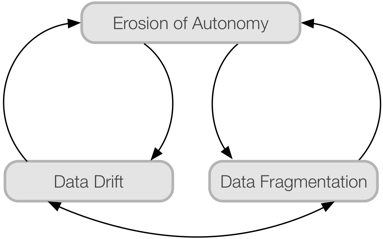
\includegraphics[scale=1.00]{figures/dbd.png}
  \caption{Cycle of Disempowerment}
  \caption*{The influence of external actors on data practices erode organizational autonomy and precipitate data drift—the altering of metrics in response to shifting requirements—and data fragmentation—the dispersal of data in non-coherent systems and schemas. These mutually-reinforcing consequences further erode autonomy leading to a cycle of disempowerment.}
  \label{fig:dbd}
\end{figure}

Autonomy of the organizations in this study is impinged upon from the start by external stakeholders---especially, but not limited to, funding agencies---whose ideas about what measurable impacts are deemed valuable implicitly or explicitly shape data practices through prescriptions of what metrics organizations should track, what information systems (owned by whom) should be used to collect M\&E data, and how such data should be reported. Data analysis is conducted by outsiders and consultants, disconnected from the organizational mission and from the organizations’ long-term vision of social impact. Data and reports are compiled in the systems of ever evolving rosters of funders, often outside the control of the organizations themselves. Taken together, these data practices eroded organizational autonomy, dictating how already over-worked staff should allocate their limited time for data practices, leading to \textit{data drift} and \textit{data fragmentation}.

This \textit{erosion of autonomy} contributes directly to \textit{data drift}---the shifting of metrics and data collection foci in response to externally re-framed missions and priorities, moving the organization towards a mission that is both undefined and unknowable. \textit{Data drift}, in turn, contributes towards an even greater erosion of organizational autonomy, as the data the organizations are left to work with moves them farther and farther away from their core mission and expertise.

The erosion of organizational autonomy also contributes to \textit{data fragmentation}---where issues of power dynamics, a reliance on external expertise and frequent stakeholder turnover lead to a proliferation of disconnected data sets. And yet, the more fragmented the data becomes, the more reliant organizations become on external expertise to fix the problem, further undermining organizational autonomy.

\textit{Data fragmentation} and \textit{data drift} are also mutually reinforcing. As the data that is collected changes over time, \textit{data drift} contributes to both longitudinal and logical fragmentation by introducing data sets that are dissimilar to previously collected data. As new types of data are collected---especially if mandated by new funders---\textit{data drift} also leads to locational fragmentation, as data is collected in or moved into new and different funder systems. Looking back the other way, \textit{data fragmentation} may also lead to \textit{data drift}, as different outside experts logically fragment data by periodically shifting focus from one set of metrics to another, resulting in a changing organizational identity as represented by their data. As the data makes less sense due to its fragmented state, the organization loses the ability to systematically understand the differences between their current and prior data environments.

These challenges compound and loop back on each other to reinforce a cycle of disempowerment overlaid on M\&E practices that are, themselves, in a near-continual state of flux. This cycle results in these organizations having an ever- decreasing role in designing their data strategy, executing their own vision, and making meaning of the data that they spend much of their constrained time collecting.

\subsection{Data Driven for Whom?}

The \textit{cycle of disempowerment} sheds new insights into the enactment and consequences of current implementations of data-driven decision making. Organizations are under great pressure to adopt data-driven decision making strategies (e.g., \cite{Haskins2011Building}). And there is some evidence, especially from the private sector, to suggest that data-driven decision making can be impactful \citep{Brynjolfsson2011Strength,Lavalle2011Big}. Yet, there are many concerns about the potential of data-driven practices in the mission-driven space, with various scholars raising possible explanations for the challenges observed: that organizations may not be adept or confident enough to use data effectively \citep{Maxwell2016Data} and that metricization is not appropriate for the mission-driven nature of organizations in this sector \citep{Benjamin2014Programs}.

What the \textit{cycle of disempowerment} foregrounds is that each of these explanations fall short of explaining why data-driven processes are not working. The M\&E professionals in mission-driven organizations are quite articulate about what kinds of data could be useful in evaluating their programs; they are invested in the work of trying to better understand how to measure impact in some of the most complex and thorny situations. Most individuals we interviewed believe that data \textit{could} be useful.

Yet, we find that the achievement of a data-driven culture is currently an impossibility—beyond the problems introduced by any particular analytics tool that thwarts the actionable use of data \citep{Verma2016DrillDown}---rooted in a more pernicious set of power relations among stakeholders. Here we find that data tools and practices are not constituting relations that newly empower organizations. Rather, data tools and practices are re-entrenching existing social relations, and making them harder to work around. Relationships with funders, for example, are being reified and reinforced through the adoption of their systems for data management---leading to increased fragmentation—and their metrics of impact and success---leading to \textit{data drift}.

This research raises the question of “data-driven for whom?” The acute political imbalance that disempowers the organization and its own expertise suggests broader implications about what may be happening more or less invisibly in so-called successful exemplars of data practices (e.g., \cite{Brynjolfsson2011Strength,Lavalle2011Big}). If data practices serve those who make decisions about what data to collect and how to collect it, and definitions of success shift to align with the metrics that are measured, the positive outcomes of data-driven decision making risk being self-reinforcing. Researchers are beginning to key in on the fact that certain metrics are being over-reified in ways that re-define what constitutes success, especially in health settings \citep{Pine2015Politics,Pine2015Emerging}. As the construction of health becomes tightly bound up in particular metrics—--e.g., heart rate, blood pressure—then interventions in response to changes in those metrics will always appear to result in better health outcomes. Yet, if health was understood in other terms, then acting on the data that these metrics offer---striving to keep heart rate or blood pressure within a certain target range while ignoring other effects---may \textit{not}, in fact, produce positive outcomes for patients.

Given the \textit{cycle of disempowerment} in mission-driven organizations, we are concerned that their \textit{data drift} might move organizations towards increasing alignment with metrics about the health of their programs and services that stand to be similarly self-reinforcing—that organizations will appear to be more ‘successful’ over time as they abandon and re-shape their mission to the terms of the data at hand. This is the pernicious consequence of \textit{data drift}, that it changes the potential futures that the organization might have. It also changes the potential futures for those clients, constituents, and beneficiaries served by the organization.

\subsection{Disempowered at Whose Expense?}

What is strikingly absent from the data in this research are discussions about the role of client, constituent, and beneficiary feedback in the evaluation work of mission- driven organizations. This absence is particularly striking because the preponderance of mission-driven organizations provide direct products and services to individuals who are, themselves, already marginalized. The only instance in this research of M\&E professionals discussing constituent feedback in their work practice emerged from a participant reflecting on the lack of constituent feedback, which she attributes to challenges in technology adoption. While P3 believes that there are appropriate tools available to help organizations collect constituent feedback, in her view, “...the problem is adoption. How do we get people [organizations] to care about this and use these tools?” (P3)

There is ample evidence in the HCI literature about adoption challenges that derive from inequalities between who does the work and who benefits \citep{Grudin1994Groupware}, and this likely plays a role. However, our research suggests that the non-use of tools that would support constituent data collection is not simply a lack of \textit{caring}. Our research suggests that the disempowerment of clients, constituents, and beneficiaries---through not having a voice in the M\&E practices of mission-driven organizations---is likely a result of the disempowerment of the mission-driven organizations, themselves: staff pressured to navigate a complicated web of actors that perpetuate a cacophony of data demands, drawing them away from the centrality of their mission as embodied by and through constituents. As M\&E work becomes further institutionalized and as metrics for evaluation stand to become standardized in the infrastructures of organizations and their funders, this is the time for calling out the disempowerment of clients, constituents, and beneficiaries at the hands of externally prescribed data practices.

\subsection{Designing to Disrupt the Cycle of Disempowerment}

In the early 1800s, statisticians from the French Bureau de Statistique undertook one of the first comprehensive national censuses, sending questionnaires to each départment \citep{Porter1995Trust}. Yet the Bureau “quickly learned that no single set of categories could be adequate” and asked local authorities to supplement the national census categories with locally- defined categories. As Porter writes, drawing on Bourget’s earlier work, “‘recognizing the existence of a diverse, local reality, irreducible to the categories of a national accounting’ was a damaging concession” to the viability of a purely nationally framed census (\cite{Porter1995Trust} quoting Bourguet).

The tensions between uniform metrics and the metrics that derive from and reflect local experience, then, are not a new problem. Yet as evidenced by the recent surge in scholarship on this topic at CHI and CSCW, it remains a thorny problem for researchers to figure out how to address in new ways \citep{Bowker2000Sorting,Pine2015Politics,Voida2017Currencies,Verma2016DrillDown}. Through our study of the work practices of M\&E professionals, we see quite distinctly the negative organizational outcomes of these tensions being resolved---as is currently—without sufficient local input. Any disruption of the \textit{cycle of disempowerment} is likely to require granting some autonomy in data practices to organizations. And yet, disrupting the cycle would require disrupting entrenched relationships among funders, organizations, ratings agencies, and others, as power is constituted through these relationships. But what researchers can do is tell stories about data practices and their presumably unintended consequences on organizations. Researchers can convene groups of stakeholders for participatory design workshops to engage in dialogue about data and undertake collaborative processes of commensuration (see \autoref{ch:wkshp}).

But we also see a critical role for researchers and designers in designing new data systems that help individuals and organizations work around imperfect and incomplete data. The design of information systems used in the mission- driven sector nearly always lock organizations into fixed schemas and demand a complete year-on-year set of data. Nearly all M\&E professionals who participated in this research believed that imperfect or incomplete data was generally useless for developing a longitudinal or comprehensive analysis of social impact. But whether the data collected and managed evolved through \textit{data drift} or through evolving understandings of what metrics were important to capture, nearly all organizations in this study reported changes to their data over time. And surely there is a broader design space worth exploring for supporting evidenced-based research about social impact without over proscribing the mathematization of ‘data’ or requiring perfect statistical inputs. What would it look like to build data systems from a sociological or historical perspective, for example? What would it look like to build data systems that drew on tools of interpretivist traditions that might not require psychological or mathematical ideals of explanation to enable M\&E professionals be able to learn things useful about the work of their organization?

\subsection{A Note About Our Use of Disempowerment}
Although our analysis of data from interviews with M\&E professionals suggests that these organizations are currently caught in a \textit{cycle of disempowerment}, we do \underline{not} see any evidence that these organizations should be relegated to a permanently marginalized standing with respect to data. And indeed, scholarship in community-based research warns against labeling communities as “damaged,” as these labels stand to further contribute to marginalization and disempowerment \citep{Tuck2009Suspending}. We do not intend to suggest that mission-driven organizations or other stakeholders discussed in this paper are damaged. Indeed, the M\&E professionals who participated in this research have significant expertise and it is essential to find ways that this expertise can be given the weight it deserves. Our intent, then, is to draw attention to the cycle so that we are better able to move beyond it.

\section{Conclusion}
In the context of monitoring and evaluation, where the role of data stands to be most tightly aligned with the mission of the organization and the passion of its employees, data practices are all-too-often experienced as busy work. For the participants in this research, data practices are predominantly experienced as a production for others that might happen at scale, but that is disconnected from any localized meaning or value and isolated from the complexities of the social situations these organizations operate within.

Mission-driven organizations serve critical social roles. However, the disempowerment of organizations in this study suggests that the cards are stacked against the very organizations that our communities rely upon. As staff get caught up in the demands of data practices, autonomy is eroded, data is fragmented, and the organization begins to change through \textit{data drift}. These consequences come together to result in organizations that are neither empowered nor equipped to think and plan for the long term, despite our communities’ needs for such strategic planning.

In this research, we have made the following contributions:
\begin{enumerate}
	\item Provided an empirical account of the data practices of monitoring and evaluation professionals in mission-driven organizations;
	\item Identified three negative consequences of current monitoring and evaluation practices: \textit{erosion of autonomy, data drift,} and \textit{data fragmentation;} and
	\item Identified relationships among these consequences, demonstrating how they collectively reinforce a \textit{cycle of disempowerment} for the mission-driven organization.
\end{enumerate}

There is promise for the role of data in the monitoring and evaluation work of mission-driven organizations. Yet, this study of data practices demonstrates that this empowering use of data is currently thwarted. Now—at this opportune cusp when new practices are starting to collide with the new-to-data-driven-decision-making value orientations of the mission-driven sector—is the time for intervening in ways that might support and empower mission-driven organizations in their use of data.
























\singlespacing \chapter{Aggregation, Identifiability, and Anonymity}  \label{ch:pk}
\doublespacing \section{Preface}
This chapter was published in issue 3(CSCW) of the Proceedings of the ACM on Human-Computer Interaction journal in November 2019. It was titled ``The Coerciveness of the Primary Key: Infrastructure Problems in Human Services Work'', and was co-authored with Lehn Benjamin and Amy Voida (author order was Bopp, Benjamin, Voida). It is included here as published with the permission of my co-authors.

\section{Introduction}
The primary key is one of the first concepts covered in introductory database design texts. The premise is simple enough: every record or row in a table should have some number or string that can uniquely identify it. Primary keys are essential for linking data spread across database tables and for looking up and retrieving data from specific records. Sometimes primary keys are relatively unique and anonymous numeric strings (e.g., a client ID number) and sometimes primary keys are less anonymous (e.g., a U.S. Social Security Number) or even less unique (e.g., a first and last name). Yet for a special instance of an identifier---a data point that establishes a connection to an object or individual---that seems so straightforward and uncontroversial, we find myriad ways that this unassuming bit of infrastructure has an outsized influence in human services work. What are the implications, for example, when an individual client is assigned two different client ID numbers by separate, incommensurate databases, each one required by a different funder of the human services organization? What are the implications when an individual client provides different pseudonyms to different human services organizations that want to aggregate her/his data to improve service provision within a community?

Through case studies of the organizational networks of two nonprofit human services organ- izations---including 37 interviews with 43 staff members from an HIV/AIDS service organization's network and a homelessness service organization's network---we find that different stakeholders use variants of identifiers and primary keys to support work practices that are far more complex and social than the linking of tables or the lookup of data. Yet we also find that the low-level, technical properties of the primary key---including that the primary key cannot be changed, cannot be null or empty, and must be unique within its context---are bubbling up through the infrastructure and forcing end-users to work on the infrastructure's terms, a class of infrastructure problem that \citet{Edwards2010InfraProb} call \textit{interjected abstractions}.

In this research, we take a broad-based, work practice approach to the study of a specific facet of information infrastructure. Instead of bounding our unit of analysis around a given technology (e.g., the relational database and its primary key), we bound our unit of analysis around what we call \textit{database practices} and \textit{primary key practices}.  This more expansive unit of analysis enables us to consider work practices that should inform system design but that do not currently rely on the technologies in question. We mirror, in particular, Voida et al.'s  study of nonprofit sector database use that interrogates not just databases that are `technically' databases, but that also include spreadsheets and paper forms used as databases \citep{Voida2011Homebrew}.  We similarly expand our analysis of the primary key to include the myriad identifiers in whatever kind of information system they might appear that are used to support primary key work practices such as organizing, sorting, linking, and accessing records. Given this approach, we use the terms `database' and `primary key' with a limited degree of rhetorical elasticity in the work presented here---sometimes stretching their original technical definitions, but within the bounds of related practice. In taking up this unit of analysis and its related rhetoric, we are able to more holistically and empirically interrogate the tensions between the work for which stakeholders are appropriating primary keys and other identifiers and the influence of the technical infrastructure on that work.

\section{Literature Review}
\subsection{Infrastructure \& Infrastructure Problems in Human-Centered Computing}
Information infrastructures are as old as the stones used by the British Empire to count their subjects \citep{Verran2001Science}. While the power dynamics between those who define what \textit{counts} for being counted and those who are \textit{themselves} counted has continued to be a pervasive attribute of information infrastructures (e.g., \citep{Martin2009Counting,Nelson2015Counts,Scott1998Seeing}), the material forms of those infrastructures have continued to evolve \citep{Dourish2017Stuff}. From stones \citep{Verran2001Science} to census tracts \citep{Scott1998Seeing} to spreadsheets \citep{Dourish2017Stuff,Vertesi2019Affordances} and databases \citep{Dourish2017Stuff,Manovich2002Language}, the materialities of information infrastructures shape work practice \citep{Dourish2012Media,Orlikowski2010Sociomateriality}. And particularly so in a contemporary society that values data-driven thinking and decision-making.

Researchers have focused extensively on characterizing the sociotechnical nature of information infrastructures, particularly its classification systems (e.g., \citep{Bowker2000Sorting,Bowker2000Bio,Bjorn2007Health,Moller2011Layers,Randall2011Distributed}) and systems of measurement (e.g., \citep{Pine2015Politics,Voida2017Currencies,Berg1997OfForms}). As Star asserts, if you overlook the social and political nature of information infrastructures, you miss ``essential aspects of aesthetics, justice, and change" \citep{Star1999Ethnography}. For example, while the process of filling out a death certificate and declaring a cause of death may seem to be factually straightforward, the information infrastructure around this task is imbued with religious and ethical values as well as influenced by doctors' work practices \citep{Bowker2000Sorting}. Additionally,  \citet{Voida2017Currencies} argue that the selection of particular units of measurement is highly political and prioritizes the needs of certain stakeholders over others, which is especially difficult given the asymmetric power relationships in the human services context. Systems of classification and measurement exert clear political influence, then, over human experience. The experience of marginalization through systems of classification and measurement is pervasive enough that Bowker and Star have given a name to the experience, calling it torque: ``the twisting that occurs when a formal classification system is mismatched with an individual's biographical trajectory, memberships, or location" \citep{Bowker2000Sorting}. Indeed, as Mol has argued: ``The point of asking what is being counted is not to argue that counting is doomed to do injustice to the complexity of life. This is certain. The point, instead, is to discover how and in what ways" \citep{Mol2002Cutting}. 

These systems of classification and measurement, when implemented in database systems, are formalized by those databases' schemas. The database---as infrastructure---then, imposes an additional requirement on the schema, that one field be declared the primary key to do the additional work of organizing, sorting, linking and accessing records. Although not often the focus of sociotechnical research in information infrastructures or classification systems, analytic interrogations of the database's primary key are one way to gain new insights into the functioning and implications of database systems. Raley notes the key role played by the primary key in linking records about an individual across databases: ``...provided a set of different databases are networked and provided that they share the same means of establishing individual identification, so that a single unit (an individual or number) can be identified consistently across a range of data sets with a primary key" \citep{Raley2013Dataveillance}. And \citet{Ribes2013DataBite} further foreshadow the critical role of the primary key in linking data back to the real-world construct(s) that those data are intended to represent---in their case, the primary key provides the crucial link between a water sample and a specific stream. While the stream's primary key is simple and mundane, if the identifier were to become detached from the rest of the data, the entire system would break down because scientists would be unable to associate the water sample with its source.

Information infrastructures are particularly essential objects of study for the fields of computer-supported cooperative work and human-centered computing because they are performative; that is, the infrastructures, themselves, exert influence on the world around them. As Bowker asserts, ``the database itself will ultimately shape the world in its image: it will be performative" \citep{Bowker2000Bio}. This performativity has been studied in many contexts including environmental monitoring \citep{Ribes2013DataBite}, flora and fauna \citep{Bowker2000Bio}, medicine \citep{Pine2015Politics}, and emergency food systems \citep{Voida2017Currencies}. As Pine and Liboiron have argued, the influence of data tools and practices are crucial for human-centered computing researchers and designers to take into consideration: ``Since computing technologies such as databases, algorithms, and information entry interfaces, are designed around measurement; the development of measurements and the politics they embody can shape HCI design before it has even begun" \citep{Pine2015Politics}. And as Taylor has argued, systems design and implementation is also a process of `world making' \citep{Taylor2015AfterInt}. Design decisions matter not just for the affordances of the final artifacts, but in the assumptions they perpetuate about what is possible in the world and for shaping the kinds of futures that people imagine, advocate for, and work towards \citep{Taylor2015AfterInt}. Within the nonprofit domain, \citet{Voida2017Currencies} argue that the database systems used by organizations and tuned to collecting particular data based on external stakeholder needs become performative by shaping ``the future of the organizations and institutions that we rely on to promote the public good and remedy social injustice." And critically, the impact of information systems on public policy may be felt unevenly by stakeholders who are powerful enough to define categories and schemas, and those---often clients---who are not \citep{Bowker2000Sorting,Star1996Ecology}. 

Because infrastructure underlies many systems layers in the design of computing, what Star and Ruhleder refer to as its ``embeddedness'' \citep{Star1996Ecology}, infrastructure has an outsized influence on system design and user experience; it is ``sunk'' into, inside of, other structures, social arrangements and technologies" \citep{Star1996Ecology}. \citet{Edwards2010InfraProb} characterize three ``infrastructure problems''  that derive from this design influence. First, infrastructure can create problems of \textit{constrained possibilities}, in which ``design choices taken by the infrastructure may preclude entirely certain desirable user experience outcomes." Second, infrastructure can create problems of \textit{interjected abstractions}, in which ``technical abstractions in the interface may appear in the conceptual model exposed to users." Third, infrastructure can create problems of \textit{unmediated interaction}, in which ``users may have to interact directly with the infrastructure to accomplish their goals." These infrastructure problems, largely unpacked by \citet{Edwards2010InfraProb} as challenges for user interface design and user experience, harken back to considerations of the materiality of information infrastructures \citep{Dourish2017Stuff}---that the embeddedness \citep{Star1996Ecology} of the technical abstractions is, itself, a reflection of the materiality of information. It is this theoretical bridging among multiple uses and audiences of the term ``infrastructure'' that we return to in our discussion, as it provides a productive vantage point for interrogating the infrastructural abstractions that force human services staff to work in their image. 

This research also responds to Bietz and Lee's call for a richer understanding of how collaborative work is infrastructured by information ecologies comprised of multiple databases \citep{Bietz2009Collaboration}:

\begin{quote}\singlespacing The tendency to dismiss situations where organizations depend on imperfectly interoperable databases as merely inefficient legacy systems is likely glossing over insights about just how multiple databases support not only different types of work but also different perspectives and priorities \citep{Bietz2009Collaboration}.\end{quote}

Here, we unpack how the micro-scale player of the primary key has an outsized influence on human services work practices across the proliferation of databases \citep{Voida2011Homebrew} of the intra- and inter-organizational work of human services provision. In doing so, we highlight the importance of focusing analytic attention---not just on those infrastructures that might otherwise be rendered analytically invisible---but on the technical assumptions underlying the material instantiations of those infrastructures. 

\subsection{The Data Work of Human Services Provision}

Human services organizations are organizations ``whose principal function is to protect, maintain, or enhance the personal well-being of individuals by defining, shaping or altering their personal attributes" \citep{Hasenfeld1974Human}. Human services represent the largest portion (73\%) of United States federal spending---providing critical services such as workforce development, healthcare, and child welfare \citep{Desilver2017Fed}. But rather than provide many of these human services directly, over the last fifty years, federal, state and local governments have increasingly contracted with nonprofit organizations to provide these services \citep{Smith1993Contracting}.  For example, the Urban Institute estimates that in 2012 governments paid close to \$81 billion to human services nonprofits for service provision \citep{Pettijohn2013Urban}. With this funding has come increased expectations for accountability and evidence of impact, which inevitably means collecting data, which we have referred to elsewhere as \textit{data compliance work} \citep{Benjamin2018Policy}. This pressure from funders runs alongside nonprofit professionals' own need for data that will help them identify problems, adjust practices, and coordinate with other providers to better meet the needs of individual clients. 

But collecting and using this data to meet these external and internal demands is not as straightforward as it seems, in part because the data needs of funders and the data needs of human services staff are often different \citep{Benjamin2008Risk,Benjamin2012FrontOut,Ebrahim2003NGOs,LeDantec2008Trenches}. Even when the same data could be used to meet both sets of needs, the data infrastructure requirements of funders make it almost impossible to do so \citep{Benjamin2018Policy,Bopp2017DbD,LeDantec2008Trenches,Ebrahim2003NGOs}.  Consequently, most human services organizations focus on meeting funder data demands often at great cost and often without a clear benefit to the people they serve \citep{Benjamin2008Risk,Carman2007Evaluation,Ebrahim2003NGOs,Snibbe2006Drown}. All of this data work rests on top of limited technical capacity and resource constraints that make the vision of data-driven human services provision outside the reach of most organizations \citep{Benjamin2018Policy,Bopp2017DbD,Burt2000ICTs,Burt2003NewTech,LeDantec2008Trenches,McPhail1998Caveat,Merkel2007NPOMethods,Merkel2004PD,Voida2011Shapeshifters,Voida2011Homebrew,Voida2012VolCoord}.

In the past several years, data demands have gotten even more complicated for human services organizations, as they are now asked to aggregate data across organizations to track progress in addressing problems at the community-level \citep{Benjamin2018Policy, Bopp2017DbD, Erete2017EmpPart, Maxwell2016Data,Verma2016DrillDown}. Here, new data issues have emerged, requiring what we have referred to elsewhere as \textit{data coordination work} \citep{Benjamin2018Policy}. \citet{Schoech2010Interoperability} has predicted that the general trend toward big data will require human services organizations to develop greater interoperability of data systems and that this will require ``predetermined data definitions, standards, protocols" and ``user authentication and identity management tools to ensure data security, client privacy and confidentiality."

Privacy concerns add additional layers of complexity to the information infrastructures in some organizations that are legally mandated to ensure confidentiality. Even in other settings, where confidentiality is not legally required, privacy concerns strain the relationships that organizations have with clients as clients raise concerns about their rights in this new data sharing environment \citep{Sparks2010Broke}. Although it is difficult to generalize about human services organizations given their diversity, on the whole, they tend to be more professionalized and bureaucratic than other nonprofits and, consequently, clients have less control in the organization, including over their data \citep{Hasenfeld2010Orgs}. Further, in human services work, data collection and service provision occur simultaneously, rendering clients' conditions---homelessness, mental illness, HIV positive status---more visible and open to inspection, visibility that is all the more acute when the client is experiencing a socially stigmatized condition. The asymmetric power relationship foregrounded by the provision (or not) of services is a powerful frame for the experience of data collection (see also \cite {Borchorst2011You}). Clients often respond to mitigate this new vulnerability by limiting what they disclose \citep{Sparks2010Broke}. \citet{Carnochan2014Performance} and \citet{DeWitte2015Street} found that collecting valid data, then, depends on working to build trusting relationships with clients---what we have elsewhere referred to as \textit{data confidence work} \citep{Benjamin2018Policy}---so that clients are willing to fully disclose information about themselves. Finally, although data collection processes can and do vary across human services settings, in many human services organizations these data collection processes are extensive and so intertwined with service provision that they almost become the service, itself \citep{Benjamin2018Policy,Soss2011Discipline}.

Additional challenges of data work in human services provision also include the following: competition among organizations \citep{Stoll2010Interorg,LeDantec2010Boundaries}, evolving priorities in public policy and associated funding \citep{Benjamin2018Policy}, and the various ways that ``doing good" can be operationalized \citep{Benjamin2012FrontOut, Voida2014SharedValues}. 

Overall, there is a significant need to understand the role and challenges of data-driven work in the nonprofit and human services context. As the pressure for these organizations to become more data-driven intensifies (e.g., \citep{Haskins2011Building}), significant questions have arisen about the effects of data-driven work practices on these organizations, their staff, and the clients they serve \citep{Benjamin2008Risk,Benjamin2012FrontOut,Benjamin2018Policy,Bopp2017DbD,LeDantec2008Trenches,Ebrahim2003NGOs,Carman2007Evaluation,Snibbe2006Drown}. Researchers have started to piece together a puzzle of various factors that are influencing or positioned to influence the nature of data-driven work in this context, including the influence of funders (e.g., \citep{Benjamin2008Account,Bopp2017DbD,Cutt2000Accountability,Ebrahim2003NGOs,Stoecker2007Research,Smith1993Contracting}), other organizations in the surrounding networks \citep{MacIndoe2013Shape}, and the public policy field \citep{Benjamin2018Policy}. This research contributes a missing piece to the puzzle in this line of scholarship: exploring how information infrastructure and its abstractions influence data-driven work.

\section{Methods}
We conducted case studies of the organizational networks of two human services organizations---one in the HIV/AIDS services policy field and one in the homelessness services policy field---to better understand the information ecosystems of data work in the nonprofit sector. Elsewhere, we present findings related to the macro-level influences that the broader policy field has on information infrastructures and work practices, including the ways that federal policies are implemented at the state and local level, the choice of funding tool used, and the assumptions about public policy problems and solutions \citep{Benjamin2018Policy}. Here, we turn to interrogate the role of a much more micro-level player, the database primary key, in the data work of human services organizations. 

\subsection{Case Selection}
We selected two organizational networks in which we anticipated that the phenomenon of interest---the data work---would be rich and intense \citep{Patton2002Qualitative}. We used three criteria to select a focal organization for each network: (1) a nonprofit that received government funding to ensure that the information ecosystem would be undertaking \textit{data compliance work}; (2) a nonprofit working in a policy field where there was an effort to achieve community-level outcomes to ensure that the information ecosystem would be undertaking \textit{data coordination work}; and (3) a nonprofit serving a population that faced some societal stigma to ensure that the information ecosystem would be oriented toward \textit{data confidence work}. We chose focal organizations working in two different social service areas (policy fields), so we could understand the degree of transferability of findings across service contexts. 

One case centers around the information ecosystem and organizational network of an HIV/AIDS services organization. The focal organization in the HIV/AIDS case is a community organization in a county with a population of approximately one million people. Like many other community organizations founded in the late 1980s in response to the AIDS crisis, this organization has a diverse portfolio: service provision for those diagnosed with HIV/AIDS, including case management, mental health and addiction counseling, and medical services; free testing and risk-reduction counseling; and advocacy for the rights of persons living with or affected by HIV/AIDS. At the time of the study, the organization had nearly 50 staff members, had served approximately 1,200 HIV positive individuals, and had provided approximately 3,500 free HIV tests. The organization had received support from a range of foundations and donors, though the majority of its funding (62\%) had come from county and state government. 

A second case centers around the information ecosystem and organizational network of a homelessness services organization. The focal organization in the homelessness case, also founded in the late 1980s, is situated in a county with a population of about 400,000 people. This organization is one of three in the city that provides services to adults experiencing homelessness, including street outreach, overnight sheltering during the winter months, and transitional and permanent supportive housing year-round. At the time of this study, the organization also had approximately 50 staff members and 2016 census figures suggest that the organization contributed to serving a population of approximately 700 homeless individuals in the county, though these census figures are widely considered to under-represent the population \citep{Schneider2016Know}. The majority of this organization's revenue came from a combination of private sources (40\%) and government grants (30\%) through two city governments, the county government and, indirectly, from the federal government (as passed through a local coordinating organization).  	

\subsection{Data Collection}
We collected data through in-depth case studies within each focal organization, as well as with key informants at organizations in the focal organizations' surrounding information ecosystem. The analysis reported here is drawn from data collected through 37 interviews with 43 human services staff (\autoref{tab:parcounts}). The semi-structured interviews broadly covered topics around data collection, entry, aggregation, use, and sharing. 

\begin{table}
\small
\begin{tabularx}{\textwidth}{p{3cm}XXX}
\toprule
 &  & \textbf{HIV/AIDS\newline Services Case} & \textbf{Homelessness\newline Services Case} \\
\midrule
\textbf{Focal\newline Organization} & Frontline staff, program managers, and data\newline oversight & 15 interviews (n=17):\newline A1-A15 & 6 interviews (n=7):\newline H1-H2, H8-H11 \\
\midrule
\multirow{2}{2.5cm}{\textbf{Organizations in the Surrounding Network}} & Staff from referral\newline organizations & 5 interviews (n=6) across 4 organizations:\newline A16, A18, A20-A22 & 4 interviews (n=4) across 4 organizations:\newline H4, H6-H7, H12 \\
\rule{0pt}{4ex}
 & Staff from data\newline aggregating organizations (e.g., funders) & 4 interviews (n=6) across 2 organizations:\newline A17, A19, A23-A24 & 3 interviews (n=3) across 2 organizations:\newline H3, H5, H13\\
\bottomrule
\end{tabularx}
\caption{Informants by Case}
\label{tab:parcounts}
\end{table}

In each focal organization, we conducted semi-structured interviews with a cross-section of staff who interact in a variety of ways with the organization's data, including frontline staff in different programs who are responsible for collecting data; program managers who are responsible for reporting this data up to senior staff; and quality assurance or other staff who provide oversight of data.

We also conducted semi-structured interviews that provided a more expansive view of the broader information ecosystem across each organizational network, including interviews with staff from other nonprofit organizations that were members of referral networks, with whom the focal organization shared clients and client data, as well as with staff from organizations who were responsible for receiving and aggregating data upstream (e.g., funders). In the HIV/AIDS case, this included staff from the county and state; in the homeless services case, this included staff at a nonprofit intermediary and the county.  

This sample of informants provides a broad view of the organizational infrastructures and data work of the network of human services organizations in each case, though it does not represent the perspectives of all organizational stakeholders. For example, while we involved many frontline staff who work directly with clients on a day-to-day basis, we are unable to represent accounts of client experiences. Instead, our vantage point in this work enables us to understand how data work affects staff members' interactions with clients---the nature of their relationships with clients and their ability to render effective and supportive services to clients. 

To better understand the complexities of the information infrastructures across each of these organizational networks as well as to clarify any ambiguities or discontinuities within or across informant accounts, we also employed two additional methods of data collection, used within the context of the semi-structured interviews:
\begin{enumerate}
\item To the extent allowable by the organization, we collected data artifacts that documented the information systems experienced by and characterized by informants, including data collection forms, the data dictionaries and database user manuals that described what staff should enter into a particular database, and the websites of the vendors who supplied the information systems and/or technical assistance to the organization.
\item In each focal organization, we also worked with the person most centrally responsible for the oversight of data to develop a data journey map for that organization and its network \citep{Bates2016Journeys}---flow diagrams of how data moved into, through, and out of their organization, including information about \textit{what} data, \textit{where} those data are organized and managed, \textit{from whom} the data originated, and \textit{to whom} the data are passed off.
\end{enumerate}


We also observed coordinating meetings within each organizational ecosystem, at which service providers and funders discussed service coordination and data sharing. These data are not analyzed here but were used to help identify key stakeholders for additional interviews across each focal organization's network.

To support the distributed fieldwork of this interdisciplinary research team, the principal investigators of the larger research program (the second and third authors of this article), conducted a phase of joint pilot fieldwork at the first focal organization before the data collection effort reported here. This joint pilot fieldwork included an initial interview with a key informant, a facility tour, and two focus groups with a breadth of staff at the focal organization. We used this pilot fieldwork to develop an initial shared understanding of the setting, the work being carried out, and the infrastructures supporting this work; to begin to establish a common language around infrastructure and data work; as well as to identify common constructs of interest. Researchers then divided up the remaining data collection. Researchers met almost weekly throughout data collection to coordinate the ongoing, iterative refinement of the interview protocol and to coordinate a consistent sampling of informants across the organizational networks of the two cases.

\subsection{Data Analysis}
We analyzed data iteratively and moved between phases of inductive analysis grounded in the data and deductive analysis grounded in the research literature (see e.g., \citep{Corbin2014Basics}). To begin, we read through the transcripts for each case separately, identifying instances of data work while attending to similarities and differences across the two cases. As with most studies, more than one interpretive frame can be used to understand the data, illuminating some aspects of a case while downplaying others \citep{Ragin2011Constructing}. In our first stage of analysis, we identified themes across the data suggesting the influence of the policy field on data work practices in human services organizations and their networks (published in \citep{Benjamin2018Policy}). In our second stage of analysis, we identified prominent, cross-cutting themes related to the role of identification, identifiability, and identifiers in those same instances of data work. We report on the details of the latter analytic process in what follows.

In our second stage of analysis, researchers inductively coded all interview transcripts for any broad relationships that the data work had to themes of identification, identifiability, and identifiers. Researchers met almost weekly to discuss the emergent coding categories and the relationships among them. Through these ongoing discussions, we began to see a distinction between: (1) coding that was descriptive of work practices that were implicated in the use of identifiers (e.g., that identifiers were important in counting clients) and (2) coding that was descriptive of the kinds of assumptions about the use of these identifiers in work practices (e.g., that critical identifiers needed to be collected first). 

Our second round of coding, then, focused on distinguishing between these two broad categories of codes and developing additional granularity to our understanding of each of them. In this phase, researchers also generated memos using the guiding questions, ``What work is being supported or constrained here?" and ``What assumptions about identifiers are supporting or constraining these work practices?" Through the continued weekly discussions, particularly as supported by these memos, the role played by different variants of identifiers came to the fore, which served to highlight the workarounds of stakeholders and how the normative assumptions of the primary key---as a special and influential instance of identifier---influenced work practices. Our third round of coding focused on interrogating even more specifically what variants of the identifiers and primary keys were implicated in these work practices and what infrastructural properties were influencing both the work practices and the contextual assumptions.

\section{Results}
\subsection{Variants of Identifiers Used as Primary Keys}
\subsubsection{Variants Across a Design Space of Uniqueness and Anonymity}
In relational database design, the primary key is required to be \textit{unique} to enable information retrieval through the identification of specific records of interest and to allow relationships to be represented across tables within a database through linking and cross referencing. Primary keys are also predominantly assumed to be \textit{anonymous}, not directly identified with a person, as database design best practices commonly suggest using a numeric identifier automatically generated by the database, itself. In the human services context, however, these assumptions do not always hold. Organizations appropriate multiple variants of identifiers and primary keys---both in the degree of anonymity afforded as well as the degree of uniqueness of the identifier and/or the individual identified. Different variants have different affordances, which support different kinds of work. 

In the human services context, primary keys typically refer to a row of data in a table that corresponds to a client or establishes a link between the client and an instance of service provision (e.g. meeting with a case manager or accessing a food pantry). Informants never used the specific, technical term ``primary key"; that construct emerged from our analysis as having particularly useful explanatory power (see \citep{Halverson2002Activity}) for explaining the assumptions and constraints around the use of identifiers. Instead, informants used language such as ``unique identifier," ``ID," or they described specific types of IDs like drivers' license numbers or U.S. Social Security Numbers. Informants used similar language regardless of whether they were referring to a primary key in a database or a similarly-functioning identifier in a spreadsheet or on a form, which mirrors our broader unit of analysis, studying identifiers used for primary key practices regardless of the material form of infrastructure supporting those practices.

Through our analysis, we found that identifiers used as primary keys in this human services context vary in the degree of \textit{anonymity} they afford---the extent to which the associated client can be identified and linked back to the rest of the data. Example identifiers sometimes used as primary keys that vary along this dimension of anonymity include the following:

\begin{itemize}
\item \textbf{Anonymous Identifiers} such as randomly-generated or incremented numeric strings are maximally de-identified and generally considered to prohibit the reassociation of data with the individual represented by the data.
\item \textbf{Obfuscated Identifiers} are created through hashes of legally-identifying information to render that data less identifiable (e.g., taking the last two letters from a first name and appending the last two letters of a last name and the day of the month the individual was born). Obfuscated identifiers enable some degree of anonymity while also theoretically enabling the identifier to be re-matched to an individual---or a small group of potential individuals.
\item \textbf{Pseudonymous Identifiers} exist in fields defined to contain legally-identifying information, but may not contain legally-verifiable information. Pseudonymous identifiers may be used consistently over time, linking consistently to the same individual even though that individual might not be directly identifiable; pseudonymous identifiers may also differ over time, providing an inconsistent reference to an unidentifiable individual.
\item \textbf{Legal Identifiers} such as names and U.S. Social Security Numbers are maximally identifiable and often require an additional level of verification against government-issued documents. 
\end{itemize}

Through our analysis, we also found that identifiers vary in the degree to which they are \textit{unique}, though in two distinct ways that are highly entangled in practice: (1) in the extent to which they are unique in the context of a given database, as is typically required in the design of relational databases, but also (2) in the extent to which they reference a unique individual. Example identifiers sometimes used as primary keys varying along this entangled dimension of uniqueness include the following:

\begin{itemize}
\item \textbf{Not Necessarily Unique Identifiers} are identifiers like names that can often be linked to a \textit{unique} individual but are \textit{not guaranteed to be unique} within a database (e.g., an instance in which two people with separate records in the same database share a common name).
\item \textbf{Aliased Identifiers} are \textit{unique} identifiers with respect to the database (e.g., an anonymous identifier might have been generated when a client presented to receive services on a first visit) but that are \textit{not guaranteed to uniquely} represent a given individual (e.g., if a second anonymous identifier was generated for the same individual on a subsequent visit).  
\item \textbf{Deduplicated Identifiers} are \textit{unique} identifiers within a given database that are also \textit{guaranteed to uniquely} represent a given individual---that is, the unique identifier has also been deduplicated.
\end{itemize}
The two entangled manifestations of uniqueness become key to understanding some of the infrastructure problems that emerge in this context and so we'll return to this entanglement in our discussion.

All of the identifiers present in our data are situated at the intersection of both dimensions. That is, all identifiers have different affordances with respect to anonymity and uniqueness (e.g., anonymous and aliased identifiers, anonymous and deduplicated identifiers, legal and not necessarily unique identifiers, pseudonymous and not necessarily unique identifiers, etc.) The data does not include all possible permutations of identifiers---and it seems intuitively likely that not all permutations may be possible. But we stop short here of suggesting or creating prescriptive links between the two dimensions so as not to constrain the designerly imagination moving forward.

\subsubsection{Variants as Instantiated Across Different Classes of Information Systems}
The information infrastructures used by the organizations in this research are, like those of many other nonprofits, creative assemblages of many types of systems---referred to elsewhere as homebrew databases \citep{Voida2011Homebrew}. These homebrew databases include various enterprise-level or custom database systems; spreadsheet applications used as databases; and paper-based instantiations of databases, often forms that mirror the data-entry workflow of another database where the data will be entered later. Though the term ``primary key" is typically only used by database administrators to refer to a special class of identifiers used in formal database systems, here we extend its use to describe key identifiers that are used to the same end across the different classes of information systems that make up these organizations' homebrew databases. For example, a last name on the top of a paper form is used for filing that form in alphabetical order then and re-accessing the data it contains later. We adopt this broader unit of analysis to enable a more holistically-informative view over work practices that are likely to inform database design---which includes not only database systems but also information systems that are used to perform similar work to that which is intended to be supported by databases. In each of these classes of information systems that make up organizations' homebrew databases, identifiers are used consistently to access records of individual clients, to aggregate records, and to deduplicate records (where possible). And in most cases, these identifiers across classes of information systems serve a significant role influencing the work of these organizations, for example:

\begin{itemize}
\item \textbf{The primary key, as implemented in database systems.} The HIV/AIDS focal organization receives funding from the County and State to provide a variety of health-related services. The funding is passed down from the Health Resources and Services Administration (HRSA), an agency of the U.S. Department of Health and Human Services, to the County and State which in turn contract out to local nonprofit service providers. Per provisions of the funding relationship, the organization shares client data with HRSA via a prescribed database system. A staff member describes the relative degree of anonymity afforded by the database through an explanation of how, in this instance, the \textit{obfuscated identifier} used as a primary key is generated: ``Real data is not reported by name to HRSA, it's reported using the unique identifier. And so, you know, the identifier is generated by an algorithm that looks at first name, last name, gender and date of birth" (A17). 
\item \textbf{Identifiers that serve as de facto, human-accessible primary keys in database systems.} Another database used within this same organizational network provides a mechanism for looking up clients' work histories via the \textit{legal identifier} of their U.S. Social Security Number so that their ``work history is then documented through your taxes and how long you worked at that employer" (A3).
\item \textbf{Identifiers that serve as de facto primary keys in spreadsheets used as databases.} Three emergency housing services organizations in the homelessness case have undertaken a grassroots effort to merge their client data to try and better understand clients' use of services across organizations in the county. Once a year, each organization exports its data to Excel from the different systems each uses as their primary client database---one from Access, one from Salesforce, and one from Excel. One executive director, then, manually merges and deduplicates all records using the clients' names as \textit{aliased or not necessarily unique, legal or pseudonymous identifiers}. A staff member at an HIV/AIDS organization manages a similar process, further specifying the workflow with \textit{legal identifiers} to involve: ``I do a sort based on names and I deduplicate" (A8).
\item \textbf{Identifiers that serve as de facto primary keys in paper forms used as analog proxies for databases.} In the human services context, one of the most common paper-based ``databases" are the forms used to refer clients for services at other organizations. The HIV/AIDS focal organization uses a paper referral for numerous services: ``The mental health referrals, substance abuse referrals, legal referrals and referrals for medical case management, those are all the paper referrals. It's a 2-page referral so the first page is basic demographic information: client's name, date of birth, Social [Security Number], contact [telephone] number and what it is they need..." (A5). The lead information on page one, the data that serves the role of the primary key for sorting and accessing each form-as-record in this instance, are \textit{legal identifiers} (e.g., Social Security Number), verified through government-issued ID cards.
\end{itemize}

\subsection{The Sociotechnical Work of the Primary Key}
Never merely just a tool for carrying out the technical work of linking database tables, primary keys---and other identifiers used for primary key practices---enable numerous forms of critical social work, as well. In unpacking the social work enabled by the primary key, we begin here to employ more of the rhetorical elasticity of our broader analytic frame. Here, by `primary key,' we are most often referring both to primary keys that are `technically' primary keys as well as to identifiers that are used for primary key practices. In the human services context, the primary key enables social work related both to the individual who is identified and to the data that has been collected about that individual. Once a primary key has been created for a client, it is used by different stakeholders to enable different forms of work both within and across organizations.  

\subsubsection{Counting Clients for Accountability: Often-Estimated Aggregations}
More than any other form of work supported by primary keys, informants talk about the work of \textit{counting clients}. In the homelessness focal organization, staff explained that the count of ``how many people have stayed each month" (H10) is frequently compiled and sent to the board because of their level of interest in the information and the metric's importance in driving their decision-making (H12). Similarly, in the HIV/AIDS focal organization, one staff member discussed the kinds of common data requests that she receives: ``My supervisor [asks] `...how many positive tests did you have this month?'" (A9). The count of positive tests per month acts as a proxy for a count of clients who have been identified as HIV+ based on the assumption that only one test has been run per person. While this might be a valid assumption in many cases, informants also discussed instances in which clients obtained additional tests or nights at a homelessness shelter by providing different identifying information at each interaction.

As a staff member from a referral organization in the homelessness services network explains, a motivation for counting clients is to compare supply and demand: ``Who do we serve and how do we want to serve them? I mean that's basically... every conversation gets down to it and it's like, you know, who gets priority? What programs [do] we put emphasis on?" (H6). Using primary keys to develop counts of people in need and comparing those counts against funding allocation allows decision-makers to reallocate resources. Underpinning this logistical question, however, is the more political question of which, and how many, clients are prioritized for services.

Notably, frontline staff rarely share accounts of counting clients for their own work. Counting clients is predominantly done for reporting upward in the organizational hierarchy and outward to boards, funders, and policymakers. In the context of this reporting, staff in both cases are fiercely protective of their clients' privacy. Even if staff used less anonymous identifiers as primary keys in information systems within the organization, they frequently de-identified their client data before sharing, switching to the use of \textit{anonymous or obfuscated identifiers}: ``I enter all the information into a big database that I send to the county quarterly. And I just de-identify it, so they just have a client identification number as opposed to a name for anonymity purposes" (H9). The acceptability of this (pseudo-)anonymization practice for the receiving parties suggests that the recipients of the data are, in general, more concerned with unique counts of clients than specific client identities. 

Yet, contrary to normative assumptions in database design that a normalized, orderly, and efficient database contains one and only one unique (deduplicated) record in each table corresponding to its real-world counterpart, the normative assumption in the human services context is that primary keys are most likely to identify unique but not necessarily deduplicated records---that \textit{aliased identifiers} are an expected and everyday reality in these organizations' databases: ``...we found out after matching everyone first that although you might naively think there was maybe 5,000 or so people in the system in the course of a year, there was probably closer to 3,000 with dupes taken out, so that was a significant finding" (H12). That process of deduplication was reported to be a little like ``detective work" (H10). In instances in which records are being tracked in spreadsheets, the counting process requires manual deduplication, often through sorting, for example: 

\begin{quote}\singlespacing
\textit{A8:} And then when it comes to reporting on overall number of households served, I don't need to count that person three times because they're on that spreadsheet three times, I need to count them once for that purpose.

\textit{I:} Do you have a unique identifier that helps you do that quickly? 

\textit{A8:} It's name-based in that spreadsheet and so I do whenever I'm counting number of households, I do a sort based on names and I deduplicate.
\end{quote}

Other informants report getting in trouble for having duplicate records for clients: ``And then County catches those and smacks us on the hand for not figuring out that they're already in there because it causes dual records and then they need to verify which one is kept..." (A14). 

Duplicated client records have to be assumed to exist both within and across organizations, however, for reasons beyond any single organization's control. Multiple funders of the HIV/AIDS services focal organization each require that records of service provision supported by their funding be entered into each of their separate databases, so the same client at a single organization might exist once, separately, in each funder's database. Staff in both cases also report being aware of instances in which clients presented at multiple human services organizations with different names, or \textit{pseudonymous identifiers}, (e.g., ``you could be Joe at the shelter and then go to [another city] and be Joseph and we would never know that you're the same guy" (H1)), making it difficult to aggregate data across organizations to derive an accurate client count for larger community-based efforts. As such, aggregated counts are more-than-likely assumed to be estimates. 

\subsubsection{Tracking Clients for Effectiveness: Aspirations of Re-Identifiable, Longitudinal Client Histories}

The most common work that frontline staff wished their data and its primary keys would support, ``the holy grail of information around people, is longitudinal data" (H1). Staff across cases most commonly referred to this work as ``tracking" or ``following" clients:

\begin{quote}\singlespacing I wish we could \textit{track} every single service that an individual will use his Ryan White [benefits] for and I thought, you know, if that was incorporated into our own database we could easily track that... but we just, when we talked about it together we just realized that would be just another database. (A7, emphasis added)\end{quote}

\begin{quote}\singlespacing Our dream... we have long conversations philosophically about how do we, how do we \textit{follow} people at the shelter? How do we follow a person?  Say they've come in as an emergency client, they entered into the transition program, you know, they got kicked out or they came back, they went, they came back, got kicked out, been here 3 times or whatever, uh, which is not uncommon and, and yet it's hard to sort of follow that person.  So we had this dream of like a data entry form where you could literally follow an individual all through their trek through the shelter. (H8, emphasis added)\end{quote}

In contrast to the work of counting clients, the work of following clients was envisioned as predominantly being useful for frontline staff. Despite the overtones of surveillance, frontline staff felt that longitudinal client data, envisioned as the ``person's history" (H6), would enable them to better serve clients' needs---forming a holistic picture of what services clients have received and, implicitly, for what services they might still be eligible. Based on a similar sort of longitudinal client history that three organizations in the homelessness services case manually assembled over a year, they observed that:

\begin{quote}\singlespacing Now we have this interesting thing.... We know [our high-use clients] by name now. We can alphabetize them, we can talk to them, you know, we can start convening committees to work around, you know, what are we going to do about it.... (H12)\end{quote}

These histories are anticipated to be able to ``create efficiency" (H6) so that clients ``don't have to keep getting cycled through" (H5). One staff member specifically affirmed that these longitudinal client histories would likely be ``a little too tedious, I think, for most funders because they want the bigger picture" (H8). 

And yet, not only are there challenges in aggregating data across multiple organizations' databases with incommensurate primary keys, there is a wicked irony here with respect to who can aggregate interorganizational, longitudinal data and who sees the on-the-ground value in those data. They are not the same populations. For funding agencies, longitudinal client histories are both feasible---and in some cases (e.g., HRSA), a reality---given that funders are in a position to prescribe the use of a particular database, define the data schema, and stipulate the use of \textit{anonymous or obfuscated, and deduplicated identifiers} to aggregate data while preserving some degree of client privacy. For example, one staff member from the HIV/AIDS focal organization (A17) did reflect that the HRSA database enforced the use of consistent, algorithmically-generated primary keys by any organization receiving funding from HRSA. This technical policy affords the creation of holistic client histories---at least for internal use within HRSA. But since not all of the focal organization's clients are supported with HRSA funding, not all clients have a HRSA algorithmically-generated primary key. As a result, for consistency within the focal organization, staff must use an alternate primary key across all their clients. This complicates the re-identification and re-association of the HRSA client's record with the actual client who frontline staff would want to serve. Through the process of aggregation, the link between the data and the client represented by the data has been compromised (see also \citep{Ribes2013DataBite}).

Nafus refers to anonymized, aggregated data that can't be re-identified as ``dead data" \citep{Nafus2014Stuck}. Data organized and stored with primary keys to help ensure privacy in aggregation, then, also prevents the use of that data by the frontline staff who envision the value of leveraging these longitudinal client histories for delivering more effective services. For them, access to the longitudinal client histories that are aggregated by funders along with the ability to re-link the data to their specific client is still a pipe dream. And the prospect of creating their own databases to try and replicate these client histories is so daunting (e.g., ``we just realized that would be just another database" (A7)) that it just doesn't happen.

\subsubsection{Verifying Client Eligibility for Accountability: Exchanging Identification for Access to Services}
Whereas the client histories supported by more commensurate primary keys that would enable the re-identification of records that frontline staff envisioned would \textit{theoretically} help them better serve clients, the \textit{actual} work that frontline staff described when talking about the identifiers that served as primary keys was the work of verifying client eligibility for services. Eligibility verification was typically used to control access to services, an enactment of the political or public policy question about which and how many clients to prioritize for services. For example, one staff member of a data aggregation organization reflected that the systems are...

\begin{quote}\singlespacing ...principally organized around collecting data for the feds. So, they're very regulative in nature. So, it's you know, who's the person you're serving? Are they eligible for what you're trying to give them? What did you give them? And that's about it. And so, you don't get a lot of information at that level that helps you in the actual management of the work. Or the effectiveness of the service that you're providing. (H13) \end{quote}

For this work, different variants of identifiers are used, depending on the way(s) in which data collection and sharing is or is not specified in agreements with funding agencies, particularly to demonstrate accountability \citep{Smith1993Contracting}. For example, a staff member at the HIV/AIDS focal organization explained that one funder mandates the use of a database that requires a \textit{legal identifier} for the provision of funded services: ``I need their... name. I can't submit a test without it. I need your date of birth because that screening form that they complete, when that specimen, when you go to a doctor's office, when they... get the results, they've got to tie that result to somebody..." (A9). In this case, the requirement for a \textit{legal identifier} may further be influenced by the nature of HIV as a life-threatening virus if left untreated.

The homelessness focal organization, in contrast, is required to submit client data to the federal HMIS, but the provision of services are not contingent on these data. The priority, then, shifts to getting someone off the street: ``We don't require ID. Low bar for entry when it gets you in tonight..." (H1). So while \textit{pseudonymous identifiers} are perfectly acceptable, limited bed space at the shelter does compel the organization to limit the number of nights that any one individual stays:

\begin{quote}\singlespacing In a very just like concrete way, we can only have 160 people here a night... They can only have 90 stays unless the person is in a program and then they have to wait until the next season... So making sure that we are keeping track of who's had how many stays, so then we're not letting people stay past that. (H10)\end{quote}

Because of this, the organization also attempts to collect \textit{deduplicated identifiers}---``Right now we just, you give us a name and as long as [it is] the name you give us every time you come, that's cool, right" (H1)---though the nature of \textit{pseudonymous identifiers} only affords \textit{not necessarily unique identifiability}.

In both cases, different variants of identifiers serve as a form of currency that clients exchange for services; the variant of the identifier that is required most commonly depends on what funders stipulate, which varies both within and across cases.  

\subsubsection{Referring Clients for Effectiveness: Coordinating Service Provision through Data Sharing}
Organizations in both cases reported using data to support the collaborative work of referring clients for services across organizations, for example: ``We work with 14 different agencies... Our whole mission... is to make referrals, so we will like refer out all day long" (H6). Unlike other motivations for sharing data (i.e., counting or tracking clients), in which client anonymity is supported through the use of \textit{anonymized or obfuscated identifiers}, client referrals across organizations necessitate a \textit{legal identifier} so that the individual can be identified on handoff as the one for whom services have been requested. In both focal organizations, the referral is documented in one of the organization's own databases. The handoff to the referral organization is done via a paper form. But the one-way sharing of data doesn't fully support these organizations' work practices. In the homelessness services case, when case managers refer a client to another organization, they want to hear back from that organization: Did the client present there for services? What services did he receive? And yet case managers report that they don't generally hear back from the referral organization: ``We don't get any information back...so it's very like: out.  We rarely get anything back" (H6).

In these cases, referral forms use \textit{legal identifiers} as primary keys, for example: ``the first page is basic demographic information: client's name, date of birth, social, contact number and what it is they need..." (A5). Once the client presents at the referral organization, a new record is created in that organization's primary database with a new primary key: ``If someone left here, for example, and went to another [organization], that person's record starts completely over at that place. It's in the system but they [the case managers] can't see anything..." (A22). For the service providers, then, the referral form severs the link between the two organizations' different primary keys referring to the same client. While it might be technically feasible to use \textit{legal identifiers} to link the two organization's records, in practice, the records remain separate. In fact, this separation remains in place even when both organizations use a shared database; access-controls on database tables are often configured to prevent staff from accessing the client's records at another organization because of privacy concerns. 

Without any link back to the referring organization's primary key identifying the client, it would be difficult for the referral organization to send back data about services rendered there. Yet, if the referral did contain a link back to the primary key of the referring organization, it would implicitly or explicitly contain provenential metadata about the referral organization, which could provide unwarranted, undesirable, or illegally-disclosed information about the client. In the HIV/AIDS case, for example, A8 noted that within a database for clients experiencing homelessness, he could not identify his referred clients as originating from their HIV/AIDS organization as that would reveal the protected status of their marginalized client population. Alternately, one could rely on a third-party, trusted organization (e.g., via a data warehouse or clearinghouse) to facilitate the two-way information exchange, but that would require that all organizations agree on which primary key to use or---more likely---that third party would create new primary keys. So in solving the problem of ensuring two-way information exchange for client referrals, that third party might be likely to recreate or exacerbate many of the same problems around aggregation that have already been reported here. 

\section{Discussion: Infrastructure Problems \& the Coerciveness of the Primary Key}
\citet{Edwards2010InfraProb} argue that the attempts of researchers to create more human-centered experiences with computing systems are frequently stymied by problems with infrastructure. One class of infrastructure problems are those termed \textit{interjected abstractions}---problems in which ``low-level infrastructural concepts become part of the conceptual model of the interface" and are ``exposed to users through the applications built on top of the infrastructure" \citep{Edwards2010InfraProb}.  That is, properties of the technical substrate bubble up to the surface where they shape the user experience. These interjected abstractions, then, force end-users to work on the infrastructure's terms. Through the interrogation of the work practices supported by variants of the primary key, we find three infrastructure problems that derive from their infrastructural properties: the immutability of identifiers, the hegemony of NOT NULL, and the demand for uniqueness within and across contexts. At the end of each discussion section, we provide provocations for design related to each infrastructural abstraction. Following these three sections, we discuss the influence of these infrastructure problems on the way that public policy is enacted.

\subsection{The Immutability of Identifiers}
In relational database design, the identifier that is used as a primary key is immutable; it simply cannot be changed. Changing the primary key would break all of the links between database tables and undermine the fundamental premise of relational databases. But some of the identifiers used as primary keys or used to generate primary keys in human services provision can and do change. For example, the database that organizations are required to use if they receive money from HRSA uses an \textit{obfuscated identifier} as the primary key that concatenates gender and name into its identifier---both of which are mutable human attributes. Or a client who gets tested for HIV using a \textit{pseudonymous identifier} as primary key has to get re-tested before he can receive any other services, because a client needs to have a record with a \textit{legal identifier} verified by government identification as a primary key---and the \textit{pseudonymous identifier} used previously as the primary key cannot be updated.  

The immutability of the primary key as an infrastructural abstraction also seems to implicate how work practices around identifiers, more generally, are structured. Informants report that numerous identifiers are also treated as immutable, even though the design of the relational database would not necessarily require it. In nearly all instances, frontline staff members were not able to change key identifiers such as the ``spelling of the name, date of birth, or the sex" (A14). If a frontline staff member enters that data incorrectly or if that data changes, they ``have to call... and fess up" (A14). A data manager working with one of the HIV/AIDS organization's funder's databases concurs and confirms that, in practice, identifiers need to be changed ``a fair amount... a couple times a week." Informants report that changing identifying information cannot typically be done by escalating the issue within the organization. Requesting changes required contacting a government funding agency (e.g., ``the County" (A14)), the database administrator (e.g., HMIS (H10)), or even the Department of Motor Vehicles (A14).

\subsubsection{Provocations for Design}
While changing a database primary key is generally not recommended due to potential impacts on data integrity and database performance, it is feasible that relational databases might support ways to accomplish such a change, or at least support an alternate way of updating this information over time, such as architecting schemas that would allow for additional or alternative identifiers to be added as trust is built. That staff members have to ``fess up" to incorrect identifier data also seems disproportionately onerous and punitive given the commonality of the occurrence and the inherently dynamic nature of the characteristics upon which some keys are based. Moreover, identifying instances of incorrect data and correcting that information should be affirmed and made easier to accomplish to increase the overall validity of data.

Keeping up with the changing nature of human data is a more general problem, as Raley notes, for example: ``the errors inherent within a catalog mailing list, one of the more basic data sets, indicates how unstable that data can be: any given population is a massive moving target..." \citep{Raley2013Dataveillance}. The infrastructural abstraction of immutability limits the ability of the database to dynamically represent a changing phenomenon. Because we see instances in which a variety of identifying information might be used in the algorithmic generation of a primary key (e.g., via an \textit{obfuscated identifier}), finding ways to better support updating data across many different fields would likely be valuable.

\subsection{The Hegemony of NOT NULL}
The workflow imposed by relational database design is that the primary key must be established first---whether automatically generated by the system (e.g., by an algorithm) or entered by a staff member or volunteer. It is simply not possible to commit a row (e.g., add a new client) to a relational database without a primary key; fields that are assigned to be the primary key are prohibited from taking on NULL or unassigned values. This normative characteristic of relational databases also shapes data collection practices. Primary key fields or identifiers that are used to generate a primary key (e.g., in the case of \textit{obfuscated identifiers}) are often collected before any others, whether data is collected on paper, in spreadsheets or using an enterprise database.  

Frontline staff members that work in these stigmatized policy fields, and, as they report, their clients, are often wary of sharing \textit{legal identifiers} when they believe that information will be shared with untrusted parties. As a result, frontline staff report working carefully to build rapport and develop trust to facilitate the collection of the type of highly personal information that typically serves as a primary key (e.g., legal names or governmental ID numbers) and, therefore, is problematically requested before other information:

\begin{quote}\singlespacing There's a very large sense of trust that is needed between the client and myself in this position and I think that the rapport built with the client is done in a very calculated way and a very transparent way: `Also like just so you know up front this is what I'm going to need from you...'. There are a number of very personal things that we have to focus on and there's also trust issues, too, `cause you're asking for like social security number and all this other stuff and we're working with clientele that doesn't necessarily trust the system or authority figures or people in general. (H11)\end{quote}

Sometimes, as reported above, the requirement that frontline staff collect data up front that includes highly personal information serving in the role of primary key requires significant additional confidence-building work. One staff member in the homelessness services case even reports a sense that data collection has gotten even more personal and intense over time: ``It's gotten quite, maybe interesting is the word. I don't know but like we want to know everybody's sexuality. We want to know everybody's this, everybody's that..." (H8). When that highly personal information becomes a precondition for determining eligibility and/or receiving services, other challenges arise, such as the proliferation of \textit{pseudonymous, unduplicated identifiers} when clients provide different identifiers to different, collaborating organizations which creates challenges for counting clients or merging longitudinal client histories. In other instances, frontline staff report not wanting the requirement to collect highly personal identifiers to foreclose connecting the client with services. In these instances, they accept \textit{pseudonymous identifiers} in place of \textit{legal identifiers}, a practice which can also create other problems down the road.

The abstraction of the primary key, specifically that it is prevented from containing a NULL value, has contributed to influencing the data collection experience, most often imposing a workflow that frontloads the need to collect the most personal information first from human services clients. The multiple workarounds created---whether the additional trust-building work before the request for \textit{legal identifiers} or whether the collection of \textit{pseudonymous identifiers} in their place---complicate and reinforce existing challenges in counting, tracking, determining eligibility, and making referrals. 

\subsubsection{Provocations for Design}
The workflow imposed by the technical abstraction that the primary key cannot be NULL does suggest a few provocations for design. What would it mean, for example, if more flexible workflows were supported that allowed a client record to be created with a temporary or placeholder name so that whatever primary key is used by the database could be generated? Then, once a trusted relationship had been built, a legal name could be entered and the primary key could be updated across the database or appended to an existing record. This approach would ensure the orderliness of the database(s) while respecting the process of relationship-building and the desire of frontline staff to move quickly to provide services when the situation is warranted.

As discussed previously, updating primary keys is challenging from a technical perspective. However, even if it were technically possible to incorporate more workflow flexibility into the database, the infrastructural abstraction that the primary key cannot be NULL is still extremely complicated to navigate for non-technical reasons. Not all records in human services are stored digitally, and updating clients' identifiers across submitted forms or case notes is virtually impossible, even if the task of updating that information was deemed to be worth the investment of time. With many organizations required to perform duplicate or triplicate entry into a variety of internal databases and spreadsheets, in addition to external databases, updating information across each of these systems would likely be deemed to yield a questionable return on investment. While, perhaps, data warehouses or federated databases might seem to offer some promise, software vendors undoubtedly also feel a lack of return on time invested, since, with probably very few exceptions, such features are likely not being requested or used by their customers. As one informant explained,

\begin{quote}\singlespacing
I think the naive response to most things is: Well, we just ought to have a master system and I think that most people who have an operation in process have legacy systems and so I think there's a lot of tension between why can't we figure out ways to use our legacy systems? And, well, it's very frustrating to have to ask a question and deal with legacy system boundaries, so I think you all should just move to a new system and there's probably something that does everything, but you know there never is. So I think that is probably the place where most things stall is in that area... (H3).
\end{quote}

\subsection{The Demand for Uniqueness Within and Across Contexts}
Another requirement in designing a relational database is that the primary key must be unique---that is, within the table of client records, each primary key must appear at most once. It is then assumed that all references to a particular primary key refer to the same entity (e.g., the client record) throughout the database. There is an important distinction between the technical requirement for uniqueness among records and the lack of a technical requirement for uniqueness among people represented by those records. While the normative assumption in database design is that the uniqueness of the primary key should result in one-to-one mappings between unique primary keys and unique individuals in the real world, the technical requirements do not actually enforce this mapping. Instead, the properties of the infrastructure merely constrain the database in representing relationships between \textit{some} person and the data related to that person. And in the human services context, this merely constrained criteria for uniqueness results in a proliferation of duplicated records. In order to construct a one-to-one mapping between a unique primary key and a unique individual, the individual either needs to (or needs to want to) be able to successfully connect themselves to their single identifier consistently over time by knowing their specific primary key (e.g., a U.S. Social Security Number) or by providing identifying information that allows that primary key to be looked up (e.g., one's associated demographic data like a name and/or date of birth). 

While the technical requirement of the uniqueness of the primary key creates space for the duplication of records that is helpful in some ways---for the negotiation of trust or the expression of a lack thereof---it does create other challenges for human services work, particularly with respect to the duplication of identifiers and, as we turn to next, the merging of records across programs and organizations. Understanding the genesis of the many-to-one mapping between the multiple primary keys associated with an individual client is essential for understanding the additional challenges with respect to the uniqueness that become layered onto this mapping.

Given the infrastructural requirement that a primary key must be unique \textit{within its given context}, it also bears unpacking the role of context in that uniqueness. The variants of identifiers that are allowable as primary keys, then, are selected to be those most suited to the sociotechnical demands of each context. And it is the varied needs of each context that create additional proliferation in the one-to-many mapping between individuals and their associated primary keys---this time because of the different (sometimes incommensurate) variants of identifiers that are used in each context. For example, one organization in the homelessness services case is morally opposed to verifying \textit{legal identifiers} when they feel their job ought to be getting people into the shelter, off the streets, and out of the cold. One smaller organization in that same case explained that ``we really don't want to be in possession of people's [Social Security Numbers], so we don't do that" (H12). In contrast, the focal organization in the HIV/AIDS services case is \textit{required} to verify and collect that very same information:

\begin{quote}\singlespacing
    We had a client who---and this happens more frequently---that they give false names when they go to get tested for HIV. And she had done an intake with a person, the name that he had given... for testing was in the false name that he gave. So she had to redo the intake under the correct name because there's no way to, because that information was null and void because of the fake name (A2).
\end{quote}

Different contexts both within and across organizations have different demands and philosophical orientations to human services provision that create variation across the kinds of primary keys that are used. 

Across databases used both within an organization (often managed by different funders, for example) and across different organizations (who may want to collaborate through the aggregation or sharing of data), the different variants of identifiers used as primary keys---the variants selected as being appropriate \textit{within a context} but that differ \textit{across contexts}---create even more challenges. For example, within the context of one HIV/AIDS service organization's database, identifiable primary keys are used productively; however, once the context expands out beyond the organization's walls and across organizations, the mere association between the identifiable client and the organization (e.g., via provenential metadata) discloses a person's HIV-positive status, which is a violation of the client's privacy. As A8 explains, ``just by being affiliated with [our organization] in that database, someone could assume or make an assumption that [the client is] HIV positive."

While either of these problems might conceivably be addressed through intermediary translation tables that match and merge client records across databases---perhaps in a way that private information (such as protected health status) is limited to a small group of database administrators---the issue becomes that there are an exponential combination of contexts, each with unique work and privacy requirements, and each with a proliferation of identifiers and primary keys:

\begin{quote}\singlespacing Since we use so many different databases but we also use different client IDs for clients even within medical services like, so we have our care coordination database, CaseManager, and then we have [another database], ACAP, that we use for medical services eligibility here.... And in each of those systems, half of those clients that are in care coordination are also going to be on medical services but they're going to have a CaseManager ID and they're going to have an ACAP ID. And the same across surveillance and prevention... so surveillance, you know, they use... some kind of unique, unique identification code for each person instead of a social [security number] so it's just trying to match between the programs and the different client IDs and that sort of thing. It's difficult. (A19)\end{quote}

As the context expands out beyond any one database or any one organization to the city, state, or national levels of scale, the lack of a consistent identifier forecloses any possibility of uniqueness. As data is aggregated at different levels, the lack of primary key consistency across contexts and over time is at odds with the infrastructural abstraction.

\subsubsection{Provocations for Design}
The entangled requirements and expectations around different manifestations of uniqueness---the infrastructural uniqueness of the primary key and the more-or-less unique mapping of those keys to an individual client---is most problematic in human services when the variety of contexts in which uniqueness must be achieved span multiple databases and multiple organizations. The overlaying of these different manifestations of uniqueness in the human services context results in a working operationalization of uniqueness as \textit{primary key consistency} or \textit{commensurability across contexts}, which, as we have illustrated above, is a sociotechnically difficult problem to solve.

If the problem of entangled uniqueness were solved, such as it were, it would enable forms of human services work that require deduplication but that do not demand identifiability (e.g., aggregated client counts). But other forms of human services work demand identifiability (e.g., longitudinal client histories). Here, the overlaid requirements of entangled uniqueness and identifiability begin to more starkly conflict.

The process of deduplicating and merging records that would constitute a longitudinal client history have been characterized elsewhere as a process of assembling ``flecks of identity" \citep{Fuller2005Media} across databases. Raley refers to the resulting corpus of data that is assembled about an individual as a ``data double"---an institutionally-oriented digital stand-in for an individual person that is built by merging discrete data streams together, which can then act---and be acted upon---as if it was the human being him/herself \citep{Raley2013Dataveillance}. These data doubles come to represent clients in public policy conversations, organizational decision-making, and program management.

For the construction of the data double, the degree of anonymity of the primary key (i.e., anonymous, pseudonymous, obfuscated, legal) matters less for merging data into a single data double than it does for linking that data double to a unique individual in the real world. For example, records across multiple databases could be linked together to form a single data double if only \textit{anonymous identifiers} were used, assuming they were used consistently across contexts and over time. However, without some type of translation table to connect the data double back to the real person, this data double would be detached from the individual and largely unusable by the frontline staff who are in the best position to use these data to help clients. As identifiers increase in identifiability, it becomes easier to link the data double to a unique individual.

To accommodate this linkage, however, consistently used primary keys must also be consistently highly identifiable. This means that in order to produce deduplicated client data doubles across contexts, there would be a need to use the most invasive, least privacy-protecting identifiers to resolve ambiguities across databases. In the process of linking data to create data doubles, then, whatever privacy advantages might have been gained by using more privacy-preserving versions of primary keys would be lost. As a result, the alignment of client privacy and welfare with an appropriate degree of anonymity in primary keys should be a pivotal consideration in any specific context. 

In both the HIV/AIDS and homelessness cases, different third-party organizations were talking about or more actively working towards developing a single, centralized, data warehouse and simultaneously working to establish buy-in for such an endeavor. There was both progress towards and pushback against a centralized data warehouse in both cases. The sociotechnical tensions that have been uncovered in this research do suggest, however, that initiatives to collapse the diversity of philosophies and requirements of different human services contexts into one global, unified identifier will face significant challenges. There will remain a need for different variants of primary keys, both in terms of the degrees of anonymity and uniqueness afforded, in different organizational contexts and for different forms of human services work. The variants of identifiers and the duplication of identifiers that clients help to seed across contexts that we see in this research are also consistent with how sociologists understand the multifacetedness of identity and its resistance to being collapsed into a single, unified entity \citep{Farnham2011FacetID}. Instead of advocating for centralized, unified identifiers that remain immutable, can never be null, and are globally unique, perhaps it is possible to design primary keys that embrace the complexity of identity and its changing nature within and across varied contexts.

\subsection{Enacting Public Policy through Infrastructural Abstractions}

In the human services context, in which the pressure for organizations to become more data-driven is increasingly intense---coming from the federal government \citep{Haskins2011Building}, from other funders \citep{Bopp2017DbD,Voida2017Currencies,Benjamin2012FrontOut}, and even from cultural narratives of technological progress perpetuated by technology companies \citep{Harmon2017Fictions}---data work is not optional. But rather than being `data-driven,' \citet{Bopp2017DbD} found that organizations in the social sector are, instead, being `driven by' their data, and others have questioned whether this data work may even ``come at great cost to themselves and ultimately to the people they serve" \citep{Snibbe2006Drown}. Along with being driven by the demands of data, then, we also find that organizations and their stakeholders are also driven by the demands of the infrastructure---often required and prescribed by funders---that are used to manage those data.

The well-established politics of classification systems \citep{Bowker2000Sorting} attunes us to the influence wielded by the categories of data that human services organizations are required to collect about their clients and the services that they provide. But here we see the influence not just of the categories encoded in a schema, but also the influence of the infrastructural abstractions underlying the material form---the relational database---in which that schema is instantiated. The materiality of the relational database \citep{Dourish2017Stuff} dictates the use of a primary key, and the infrastructural abstractions of that primary key---that primary keys are immutable, can never be null, and are globally unique---in turn, force the sociotechnical work of human services provision to be carried out in its image:
\begin{itemize}
\item \textbf{Infrastructural abstractions influence the nature and order of the work.} Frontline staff members are tasked with a workflow in which highly sensitive personal data are supposed to be collected before other data---or even before services can be rendered. Frontline staff report that instead of feeling that their job is about helping clients succeed in programs, it is now just data work.
\item \textbf{Infrastructural abstractions create new forms of work as stakeholders work around the constraints of the abstractions.} Frontline staff have to call to ``fess up'' to funders when client data changes. Testers have to add re-testing to their workload for clients who originally presented with a \textit{pseudonymous identifier}. Frontline staff engage in additional trust-building work before requesting identifiers that could be perceived as too personal.
\item \textbf{Infrastructural abstractions influence the tenor of the relationships among individuals.} Frontline staff provide accounts suggesting a disempowering relationship with those who manage and gatekeep data in databases. They also report evidence suggesting that tenuous relationships with clients are dynamically negotiated through the data-sharing process.
\end{itemize}

\citet{Edwards2010InfraProb} suggest that interjected abstractions from the underlying infrastructure can lead to problems in usability and usefulness at the interface layer. Here, we find that these infrastructural abstractions have a much more coercive reach, forcing people to work in the image of the infrastructure. The relational database and its infrastructural abstractions, in some ways, \textit{becomes} the work of human services provision: ``A lot of my clients get to the point now where I'm not even asking the questions. I just say, `hey how's it going?' and they're answering everything" (A5). But even more, the relational database and its infrastructural abstractions become the de facto public policy.  Staff members relate to clients through the data they have to collect (see also \citep{Soss2011Discipline}), but also, as we see here, \textit{how they have to collect it}---where the \textit{how} is dictated in no small part by the constraints of infrastructural abstractions. When staff relate to clients through data and information infrastructures, they do so instead of relating to clients by considering their unique situation and the overall objective of the policy: to reduce the incidence of HIV/AIDS or homelessness.  

Policy, then, is not merely enacted through the classification systems and systems of measurement that are directly or indirectly prescribed by legislation produced by politicians or by contractual language drafted by funders \citep{Soss2011Discipline}. Public policy is also enacted---likely unknowingly---by software engineers who implement and maintain relational database platforms and instantiate the rules and constraints in the infrastructure that becomes coercive to the work of human services provision.

Granted, designing for human services provision will never be an entirely technical pursuit, even given contemporary demands that these organizations be increasingly data-driven \citep{Haskins2011Building, Bopp2017DbD, Harmon2017Fictions}. But the diversity of values and logics that underpin computer-supported cooperative human services provision (see also \citep{Voida2014SharedValues}), in this research, suggest that infrastructural abstractions supporting more flexibility in work would be beneficial. These flexibilities would give staff the space to negotiate the layered-ness of human relationships in this context---relationships among governments, funders, and organizations; among collaborating organizations; and between clients and each of these. 

\section{Conclusion}
Information infrastructures are, indeed, performative. The schemas and classification systems that privilege the collection and use of some data over others influence what is possible. But the identifiers and primary keys that enable the linking and accessing of those data are also performative. The technical properties that have been baked into the primary key shape work in often-coercive ways, forcing end-users to operate in the image of the infrastructure and to find ways of working around that infrastructure. In this research, then, we make the following contributions:

\begin{itemize}
\item Elaborate a design space for identifiers, including empirically-observed variants of identifiers along axes of anonymity and uniqueness;
\item Present a descriptive account of four classes of sociotechnical work afforded by primary keys and other identifiers that do the work of primary keys;
\item Identify three technical abstractions of the primary key---that it cannot be changed, cannot be empty, and must be unique---the properties of which have forced end-users to work in the image of the infrastructure;
\item Suggest design provocations for better supporting identification across a variety of contexts; and
\item Provide an empirical account of infrastructural abstractions coercively influencing work practice and enacting de facto public policy.
\end{itemize}

The data collected by human services organizations characterize some of society's most pressing social problems. These data provide accounts of the interdependence of various human challenges; chronicle the successes and failures of potential remedies and solutions; and support data-driven decision-making for individuals, organizations, and larger communities. If the identifiers and primary keys that hold information infrastructures together and that bring information infrastructures together were more supportive of the sociotechnical context of these critical data, we could engender more transformative outcomes for human services organizations, their clients, the communities they work in, the donors who fund them, as well as the policymakers and citizens who have a stake in these organizations delivering effective services. 

\singlespacing \chapter{Multi-stakeholder Questions and Assumptions} \label{ch:wkshp}
\doublespacing \section{Introduction}
Determining if we are making progress towards our goals in life is an ongoing process in which we are constantly collecting data. Organizations like businesses, governments, and nonprofits often have established milestones they seek to reach to achieve their strategic and desired goals. Organizations that are established as for-profit may have a goal of reaching a certain level of profitability so that employees can be paid. According to public administration scholars, ``public sector organizations often pursue goals that are vague and difficult to see or measure. A pizza restaurant wants to make money. It is pretty clear when it is succeeding or when it is failing. It is much harder to tell when a local housing agency is doing well'' \citep{Eller2013Public}.

While it is understood that public sector organizations have more difficulty in measuring progress towards their goals, there is less understanding of how exactly this work is approached. Nonprofit scholars and practitioners have argued that not only is it difficult to measure nonprofit work, but a ``focus on outcomes is anathema to civil society'' \citep{Brest2020Outcomes}. In this study, we asked individuals involved in public sector work---specifically the area of homelessness---to workshop their approaches to the measurement of their work at a very granular level. By asking participants to write down specific questions they seek to answer, and by circling specific fields on data collection forms, workshop participants provided a detailed account of how some in the public sector measure progress towards these often difficult and vague goals. 

We involved a total of 25 individuals in workshops across a variety of levels, from funding organization staff, to individuals who implement services as paid staff or as volunteers, to individuals who have formerly or are currently experiencing homelessness. We found that the questions that get asked fall under two perspectives. The first is the sociocentric perspective which seeks to answer questions about community-level impact, and the second is the egocentric perspective which focuses more on the experience of the individual experiencing homelessness. We observed that the sociocentric perspective is more highly valued by stakeholders for its ability to convince relevant audiences to invest in homelessness services, and to provide hard numbers that can be trusted. The egocentric perspective also has the potential to advocate for continued funding, however, this perspective focuses more on the day-to-day management of homelessness services, and suffers from its inability to present information as hard numbers.

In this paper, we will explain the types of questions that participants asked and the data they used to address each perspective. In explaining each, we will focus on the audience that the perspective aims to speak to, the capacity for decision making, and the extent to which information is knowable. Following the results section, this paper will discuss the relationship between these perspectives and panopticon as explained by Foucault. We argue that in contexts like the one examined here---where goals are vague and difficult to see or measure---rather than approaching information systems as panopticons, they should be approached as oligopticons to deal with more diverse types of data and experiences. Oligopticons foreground the necessity to approach data collection from multiple connected sites, and emphasizes that decisions must always be made based on partial data because not all of the world can be represented.

While there have been other studies in HCI that have explored crossing levels in public sector organizations (most notably \citet{LeDantec2010Boundaries} and \citet{Verma2016DrillDown}), this research makes two main contributions. The first is broader participation in terms of research participants and organizational focus. This research has brought clients (people experiencing homelessness) into conversation with nonprofit staff, volunteers, and decision-makers. In terms of organizational focus, this research has extended beyond single databases or organizations to more broadly include all information systems and organizations in the community. Secondly, this research provides a framework of perspectives that integrates with the oligopticon construct. This new orientation allows us to move closer towards designing information systems that will better support the needs of public sector users.

This research also focuses specifically on outcome assessment---which is further explained below---in order to narrow in the scope on a specific type of decision making in nonprofit organizations. We do not aim to understand data-driven decision-making broadly in this research, although outcome measurement is highly intertwined and with other types of decision-making in nonprofit organizations. In fact, ``virtually every activity engaged in by a nonprofit organization is at least implicitly intended to achieve a social or environmental...outcome" \citep{Brest2020Outcomes}. By focusing on this one type of decision in one policy field (homelessness), this research can explore these decisions at the level of detail necessary to understand such contested and difficult cooperative work. Therefore, the results discussed in this paper speak to the construction of data representations for outcome assessment only, and additional research is needed to relate this work to other types of decision-making in nonprofit organizations.

\section{Literature Review}

To support the exploration of data use by public sector stakeholders, this literature review will discuss the audience for public sector data and the challenges these audiences introduce into the data work. It will also cover the ways that different stakeholders at different levels share data and approach decision making---often in the absence of consensus. Finally, literature regarding the theoretical construct of the map and terrain will be discussed, which will be leveraged in the results section.

\subsection{Outcome Assessment Audience}
Given that many nonprofit organizations have missions to achieve social change, scholars have argued that is important nonprofits ``know how effectively they are performing their jobs. Are their programs achieving the desired results? How could programs be modified to improve those results?" \citep{Thomas2016Outcome}. The process of measuring progress towards desired results is referred to as outcome measurement or assessment. ``Used appropriately, outcome assessment...inform[s] a wide range of decisions about whether and how programs should be continued in the future and satisfy funder requirements" \citep{Thomas2016Outcome}. As this quote highlights, outcome assessment has dual purposes: decision-making about the implementation of nonprofit programs, but also to satisfy funders.

Despite the importance of outcome assessment for decision making and for satisfying funders, research has found that organizations lack adequate financial and human resources to engage in data work (e.g. \citet{Bopp2017DbD,Erete2016Storytelling}). For the work that organizations manage to do, power dynamics in the sector have prioritized funder needs for accountability data over operational data which would be more helpful to the organizations spending the time and resources on the data work in the first place \citep{Bopp2017DbD,LeDantec2008Trenches,LeDantec2010Boundaries,Benjamin2008Account,Voida2017Currencies,Stoll2010Interorg}. When organizations do not meet funders' expectations based on the provided accountability data, some funders expect organizations to provide explanatory accounts to justify the discrepancy \citep{Benjamin2008Account}.

\subsection{Decisions across Stakeholder Levels}

The nonprofit sector is not, however, only comprised of nonprofit staff and funders---there are many different levels and groups of stakeholders \citep{Bryson1995Strategic}. Focusing specifically on the area of homelessness services, the context for this study, \citet{LeDantec2010Boundaries} refers to these different levels as ``scales of influence and accountability." Information sharing occurs across and within local service providers, city and county governments, regional organizations that coordinate across cities and counties, as well as state and federal scales \citep{LeDantec2010Boundaries,Benjamin2018Policy}. Additional information exchange occurs between staff and people experiencing homelessness \citep{LeDantec2011Publics}, as well as between people experiencing homelessness and others in the community (e.g. family and friends) \citep{LeDantec2008Dignity}. Despite the information being exchanged across multiple scales, the focus on accountability and a low value placed on client privacy means that information systems are still designed to prioritize accountability to higher levels \citep{LeDantec2010Boundaries,Sparks2010Broke}.

Nonprofit staff often disagree with the way that those at the top levels have operationalized their values through these data systems \citep{Voida2014SharedValues,Voida2017Currencies}. While many stakeholders across the entire range of scales can often agree that social change is needed, the specific approaches can be more contested \citep{Voida2014SharedValues}. Research has shown that across a wide array of domains, these politics are operationalized---and therefore visible---in information systems (see e.g. \citet{Bowker2000Sorting,Bowker2000Bio,Pine2015Politics,Voida2014SharedValues,Voida2017Currencies}).

There is also disagreement among levels in terms of what counts as data \citep{Rodger2016Mobility,Verma2016DrillDown,Voida2017Currencies}. Individuals who are not as familiar with the nonprofit's work often view qualitative data as either less valuable or irrelevant \citep{Thomas2016Outcome}. However, those familiar or more deeply involved in the work feel that quantitative metrics are incorrect, especially in comparison to their own qualitative accounts \citep{Schwalbe2004HS}. While there is disagreement about the role of each type of data, many stakeholders believe that qualitative data should be used to supplement quantitative data (often framed in economic terms) in order to tell stories---especially to garner support from other stakeholders \citep{Erete2016Storytelling,Rodger2016Mobility}.

However, studies have found that this qualitative data is more than just supplemental stories, it is the essence of nonprofit work and it is largely not supported by the information systems that nonprofits rely upon \citep{Marshall2016Accountable,Thomas2016Outcome,Verma2016DrillDown}. As \citet{Thomas2016Outcome} explains, ``disdaining qualitative data further limits the ability to assess a program because the goals of most public and nonprofit programs are too subjective to be measured only by quantitative techniques" \citep{Thomas2016Outcome}.

\subsection{Map \& Terrain}
While paper maps and geographical terrain are physical objects that exist in the real world---and objects that we will discuss here---the way they will be used in this chapter are entirely conceptual. Throughout human history, maps of geographic regions have been useful because they use standardized and abstract representations that can be used by an outsider---someone who has never visited the region---to understand information about the local context \citep{Scott1998Seeing,Porter1995Trust}. Historically, these maps have been used largely for governmental management, especially taxation \citep{Scott1998Seeing}. While these maps may be useful for outsiders to manage the territory from afar for the purposes of managing revenue, these maps present a view of the territory that is ``far more static and schematic than the actual social phenomena they presume to typify'' \citep{Scott1998Seeing}. These map-level representations ignore the local context, drawing simple regional boundaries across physically impassible mountain ranges and rivers \citep{Scott1998Seeing}.

Another way of understanding the relationship between the map and the terrain is the analogy of the forest and the trees. Scientific forestry in the late eighteenth-century distinguished between trees that could be individually managed and forests that were comprised of individual trees---and therefore manageable in the aggregate \citep{Porter1995Trust}. While some, particularly naive formalists, might believe that everything that is represented at the map or forest level might be sufficient for decision-making, others have argued that decision-making should rely on not only the forest/map view but also the tree/terrain view \citep{Berg1997OfForms}.

\section{Methodology}
As explained by \citet{Bopp2019Voices} ``the prevalence of human-computer interaction (HCI) research carried out with nonprofit organizations has increased dramatically over the past 35 years,'' however, HCI researchers have more often engaged with nonprofit employees than nonprofit clients. It has also been observed that very little research has engaged across nonprofit stakeholder groups, which would help allow us to ``better understand where conflicts might occur between needs and values and can help negotiate those more explicitly'' \citep{Bopp2019Voices}. To meaningfully engage with nonprofit clients---among other important stakeholders---we designed this research to align with the values of community-based research, which emphasizes that community members should be actively engaged throughout multiple phases of research \citep{Israel1998CBR}.

To prioritize research that is important to the community, the first author attended a cross-organizational meeting between two organizations that collaborate on homelessness services and data work. This meeting included representatives from a major nonprofit organization, as well as representatives from the local county government. A major point of discussion in this meeting was the alignment of outcome metrics, a topic that has come up frequently in our prior research as well (e.g. \citet{Bopp2017DbD}). Following this meeting, we had additional conversations with staff members about a study that focused on outcome metrics. Through several iterations of study design, we determined that a focus on outcome metrics provided a unique perspective on not only a community need but also one that would address our research focus on understanding the construction and use of data representations by a diverse set of stakeholders.

Once the study design was clarified with community partners, we began planning activities for workshops in which multiple stakeholders (e.g. funders, staff, and people experiencing homelessness) would be brought together to discuss outcomes and the data-based representations that are constructed to support them. This study builds off of prior research \citep{Bopp2019Primary,Benjamin2018Policy} by focusing specifically on the domain of homelessness, adding a cross-stakeholder perspective, and focusing on the construction and use of data representations.

In this paper, we refer to our methodology as ``workshops" to indicate that participants engaged in activities that were generative in nature: writing down outcomes on index cards, sorting those cards, and comparing cards to paper data collection forms. Outside of the generative activities, discussion operated as a focus group---with a researcher acting as the facilitator to guide participants through discussion, and to encourage individuals to speak to one another about their experiences. The generative activities were designed to ground participant discussions in specific outcome metrics and data points.

\subsection{Participants}
As researchers who do not directly interact with the community of people experiencing homelessness, it would be difficult for us to establish the trust and rapport needed to recruit clients. Therefore, we began by contacting local leaders in government and nonprofit organizations to ask if staff in their organizations were interested in participating in the study. We also requested that staff members speak to clients about participating in the study.

The main funding organization in the region also included an advertisement for the study in their newsletter, which is distributed broadly across the region to many organizations and individuals interested in homelessness. All interested parties that contacted researchers were followed up with and provided additional information about the study.

Workshops included a mix of stakeholders, which are grouped in \autoref{tab:wkshp-participants} as working for an organization tasked with obtaining and distributing funding, managing front line staff and volunteers, staff members and volunteers who work directly with people experiencing homelessness, and clients who are currently or have formerly experienced homelessness. A total of 25 individuals participated in a total of 5 workshops, each with a different composition of stakeholder groups.

\begin{table}
\begin{tabularx}{\textwidth}{X|XXXXX|X}
\toprule
\textbf{Workshop} & \textbf{Funders} & \textbf{Managers} & \textbf{Staff} & \textbf{Volunteers} & \textbf{Clients} & \textbf{Total} \\
\midrule
1 & 3 & - & - & - & - & 3 \\
2 & - & 2 & 3 & - & - & 5 \\
3 & - & - & - & 5 & - & 5 \\
4 & - & 3 & 1 & - & 3 & 7 \\
5 & - & - & - & - & 5 & 5 \\
\midrule
\textbf{Total} & \textbf{3} & \textbf{5} & \textbf{4} & \textbf{5} & \textbf{8} & \textbf{25} \\
\bottomrule
\end{tabularx}
\caption{Workshop Participants}
\label{tab:wkshp-participants}
\end{table}

\subsection{Workshops}
The first author facilitated a total of five workshops, which each lasted approximately 90 minutes. The workshops took place in locations that were convenient for participants, typically within their offices, but also in their homes when invited. We provided all workshop participants with snacks and drinks during the workshop. Participants who attended the workshop on their personal time were compensated with \$20 store gift cards at the end of the workshop. An individual who has worked with people experiencing homelessness for a number of years recommended this compensation strategy, which is also consistent with approaches in similar studies \citep{LeDantec2008Dignity}.

While workshops were customized to those in attendance, the general flow of the workshop focused on two main activities:

\begin{itemize}
\item \textbf{Activity 1.} Identification and discussion of important outcome metrics.
\item \textbf{Activity 2.} Mapping and discussion of data elements from forms to the outcome metrics identified in Activity 1.
\end{itemize}

\subsubsection{Activity 1}
To start the workshop, we provided participants with eight index cards and asked them to write down four outcome metrics that are important to them personally. We customized our language to align with language that is more commonly used by those individuals. For example, in planning discussions, one volunteer explained that the language they use within their organization to refer to outcome metrics are instead ``questions that we ask about our work." This language was used throughout all workshops that involved volunteers and clients. To funders and some staff, the term ``outcome metrics" was more familiar, and was therefore used in those workshops.

Following the identification of four outcome metrics that were important to themselves, we asked participants to write down four additional outcome metrics that people other than themselves have expressed interest in, based on their personal experiences (e.g. conversations with those individuals, or requests for specific data). On the back of each index card, we asked participants to write down the stakeholders that find these outcomes important. Finally, we asked participants to examine each of their eight cards and put a sticker on each card if data is currently collected for that outcome. As will be discussed in the results section, some participants had questions about what ``counted" as data---whether those had to be formally collected statistics or not---and we encouraged participants to think broadly about data, more specifically that they should not limit their interpretation to formal statistics only, but should include data such as informal conversations.

Once these cards were created, we encouraged participants to reflect on the experience of generating outcome cards. This discussion included topics such as the identification of themes across outcomes, reasons why certain data were not collected, the difficulty or ease to which certain outcomes could be measured, and why certain outcomes were valued over others by different stakeholders. This discussion was largely participant-driven, and we only interjected with questions when the conversation slowed down or needed to be redirected back onto the topic of outcome metrics and data representations. This portion of the workshop lasted, on average, about 15-20 minutes.

\subsubsection{Activity 2}
Following the conclusion of the first round of discussion, we asked participants to do additional individual work to prepare for the second conversation. In this activity, participants were asked to select one of their eight outcome index cards---using whatever criteria they felt was important---and examine blank printed forms to find data fields that would help make decisions about their chosen outcome metric. For example, if a participant chose an outcome of decreasing the number of clients who exit homelessness programs to enter the prison system, they might circle portions of a form that asks a client where they are going after they leave the program. The participant might also need to circle portions of the form including the veteran status if part of understanding the outcome is comparing veterans with clients who are not veterans.

In line with the components of a future workshop \citep{Jungk1987Future}---which allows participants to not only critique the present but also imagine a new future---we then asked participants to use post-it notes to add additional questions to the forms if there was more information needed to fully understand the outcome that they were focusing on. Similarly, we also asked participants to cross out elements that they thought should be removed from the form.

Following this individual work, we encouraged participants to report out individually on their experiences in finding portions of the forms that supported their selected outcome. We asked follow up questions of each participant based on their response to make sure that each participant discussed the extent to which the outcome was supported by data, elements that were missing, changes that should be made in the future, and what would be involved in making those changes. After two or three participants reported out on these topics, we encouraged participants to reflect on what others were saying.

\section{Data Analysis}
As noted by \citet{Bopp2019Voices}, HCI researchers have typically foregrounded the experiences of nonprofit staff over clients, and this approach to analysis aims to address this imbalance. We started our analysis process with workshop \#4 which included discussion across the broadest number of stakeholders (including clients), and workshop \#5 which involved clients-only. By starting with these two workshops, we analytically foregrounded the experiences of people who are currently or have in the past experienced homelessness. Following the analysis of these two workshops, we analyzed the remaining workshops to add additional context from other stakeholder groups.

Our analysis process involved listening to each workshop transcript, summarizing, and time stamping participant statements so that they could be easily referred to in the future for more close transcription. When discussions were particularly rich, we transcribed these sections word-for-word during this initial analysis phase. Following this end-to-end analysis of each workshop, we applied open codes to the collected data. As necessary, we referenced workshop artifacts including index cards and modified forms to add additional depth to our open codes.

Following the initial round of open coding as described above, a total of three rounds of axial coding were completed, with each round returning to transcribed quotes to remain grounded in data. At the end of each round of coding, the first author wrote memos that discussed each axial code and then discussed these memos with the second author. The first round of axial codes focused on the representations that were limited in some way: by scope, area of concern, or in terms of the client's lived experience. The second round of axial coding surfaced a variety of assumed values including compliance, connectedness, comprehensibility, and complexity. Additional memoing on the value-based axial codes surfaced a variety of assumptions that stakeholders have about the audience for particular outcomes, the type of decision making that data supports, and the extent to which data can render a context knowable. Our subsequent memos surfaced that these assumptions fall into two different perspectives: sociocentric and egocentric.

\section{Outcome Metric Perspectives}

Workshop participants discussed their own approaches to data analysis, and while they are not conducting network analysis in the traditional sense, their questions fall into familiar frames. As discussed by  \citet{Marsden2002EgoSocio}, social network analysis often approaches data from two perspectives, the sociocentric and the egocentric approaches. The sociocentric approaches focus on understanding the complete network in its entirety by providing ``information on relationships among all nodes within a bounded social network'' \citep{Marsden2002EgoSocio}. On the other hand, the egocentric approach focuses on ``information about only that portion of a network in the immediate locality of a given node" \citep{Marsden2002EgoSocio}.

We observed that the outcomes that workshop participants discussed approach decision making across networked levels of stakeholders from either the sociocentric or egocentric perspective. Like a map, outcomes from the sociocentric perspective rely upon standardized and abstract representations to understand community-level impact. The sociocentric perspective is relied upon by outsiders (e.g. funders and the general public) to gaze upon the local context from a distance. On the other hand, outcomes from the egocentric perspective align with the mapped terrain by focusing on understanding impact on individual community members. While the specific contours of the geography are not visible from the map or sociocentric perspective, those contours are deeply embedded and essential to understanding the context of the egocentric perspective. These two perspectives are discussed further below.

\subsection{Sociocentric Perspective}
Many workshop participants discussed the need to collect data to assess outcomes from a sociocentric perspective, for example, across organizations at the level of cities and counties. To understand community-level impact, questions from this perspective include:

\begin{itemize}
\item How many people are homeless in our community and is the number decreasing over time? The annual point-in-time count answers this by conducting a census of people experiencing homelessness on a single night in January.
\item Is our system as a whole addressing the needs of people experiencing homelessness by getting them successfully housed? Success is determined by tracking the locations that people move to (e.g. overnight emergency shelter or long-term program) when they leave, or `exit', a housing program. A positive `exit' destination might be, for example, living with a relative, while a negative `exit' destination would be living on the street.
\end{itemize}

Both the point-in-time count and exit destination metrics are defined by the Department of Housing and Urban Development (HUD), the federal agency charged with overseeing much of the government-funded homelessness services in the United States. Participants from a funding organization in workshop one explained that outcomes like the exit destinations are examined at a system level through a ``racial and equity" lens by subgrouping these outcome metrics into relevant community demographics.

While the sociocentric perspective generates data that can be used to assess outcomes at a community level, as a staff member in workshop two explains, this is not the entire story:

\begin{quote}\singlespacing ``We're exiting people, and maybe it's coming up as a negative exit or a positive exit on the report, but it's not showing the context, the facts of what's happening on the date of exit. It seems black and white, but as we know people are not black and white. There's more things happening that `exited to destination' doesn't account for." \end{quote}

The contextual elements that are missing include considerations such as an individual's priorities when dealing with other things happening in their life such as relationships, mental health challenges, substance use, and employment opportunities. Analytically, this information is more of a consideration from the individual perspective, which is discussed next.

\subsection{Egocentric Perspective}
Workshop participants also discussed the need to collect data to assess outcomes from an egocentric perspective, for example, rich narratives about the challenges that an individual experiences while living on the street. In order to understand impact on individual community members, questions from this perspective include:

\begin{itemize}
\item How has this person balanced their need to meet with case managers during the day to be eligible for services while searching for employment?
\item What communities is this person part of and how does that influence their ability to search for or stay housed?
\end{itemize}

In contrast to data collected for sociocentric questions, which rely on more highly defined and typically quantitative metrics, the data used to answer this type of question requires collecting qualitative data. Participants referred to this as `soft' information and `anecdotal data' (W3), emphasizing that the data was not as trusted or valued by certain stakeholders.

Data used to address egocentric questions are not typically defined by an agency like HUD in any kind of consistent schema. A client in workshop four explained that this data is best collected by ``actually sitting down and talking to [people experiencing homelessness] to see what's going on in their lives and how they can help." This type of data is not ``track[ed] in logs necessarily" but is instead gathered through conversations with people experiencing homelessness, and is shared throughout the organization as a ``network of information" is formed through conversations amongst staff and clients (W3).

\begin{table}
\begin{tabularx}{\textwidth}{p{2.5cm}XX}
\toprule
& \textbf{Sociocentric Perspective} & \textbf{Egocentric Perspective} \\
\midrule
\textbf{Audience} & Federally mandated counts and scores can convince funders and the public of the need to continue addressing homelessness due to the scale of the problem. & The individual experiences people face should be used to convince funders and the public of the need, and the complexity, of addressing homelessness. \\ \midrule
\textbf{Decision Making} & Integrating different data sources should allow for quantitative metrics that support decisions that are aligned with the wise use of limited financial resources. & Rich qualitative data about individuals should be used to make day-to-day operational decisions. \\ \midrule
\textbf{Knowability} & The quantitative metrics discussed above constitute hard facts because the important aspects of homelessness are fully knowable. & As a disconnected individual, the person experiencing homelessness can never be fully knowable. \\
\bottomrule
\end{tabularx}
\caption{Key Assumptions}
\label{tab:wkshp-results}
\end{table}

\section{Outcome Assumptions}

Workshop participants surfaced a variety of different assumptions that were analytically placed within either the sociocentric or egocentric perspective. These assumptions---summarized in \autoref{tab:wkshp-results}---were about what audiences the data speaks to, what the data conveys to those audiences, the ways that audiences should use data to make decisions, and the ability for audiences to know and understand details about the context being assessed. Overall, participants have assumed that outcomes from the sociocentric perspective must emphasize quantitative metrics---particularly in economic terms---that can render homelessness legible to outsiders. Outcomes from the egocentric perspective instead assume that, while not fully representative, individuals' experiences can be used to better understand homelessness and support day-to-day decision making.

The designation of an assumption as either sociocentric or egocentric is not meant to indicate the physical location of decision making (i.e. sociocentric questions are not only asked by federal law makers in government buildings, and egocentric questions are not only asked by individuals experiencing homelessness on the street). Rather, an assumption's classification here as either sociocentric or egocentric refers instead to the approach an individual stakeholder takes to data analysis. For example, people experiencing homelessness made both egocentric assumptions about how to find food pantries that were open, and sociocentric assumptions about how homelessness is understood by the public.

We rely on the term `assumption' to convey several important analytic points about our observations. The first is that in presenting what workshop participants discussed, we make no assertions here as to the validity of their assumptions, but instead present them here as described to illustrate how they complement or conflict with one another. The second reason we use this term is to indicate that workshop participant's beliefs are likely fluid. While these assumptions may be true today, there is the possibility that they will change in the future as other sociotechnical features evolve.

  % % % % % % % % % % % % %
  %                       %
  % AUDIENCE ASSUMPTIONS  %
  %                       %
  % % % % % % % % % % % % %

\subsection{Audience for Outcomes}
Workshop participants discussed assumptions they make about the audience for outcome metrics. Outcomes from the sociocentric perspective focus on numbers of people experiencing homelessness, whereas the egocentric perspective emphasizes rich narratives about the challenges that an individual experiences while living on the street. Both of these metrics are used to convince funders and the general public of the need to continue addressing homelessness, however, each perspective has a different approach. The system perspective emphasizes the scale of the problem, while the egocentric perspective captures important nuance as well as the emotional gravity of experiencing homelessness by connecting more deeply with the individual person.

\subsubsection{Sociocentric Perspective Audience Assumption}

Using metrics often defined by HUD, sociocentric perspective outcomes regarding audience assume that \textit{federally mandated counts and scores can convince funders and the public of the need to continue addressing homelessness due to the scale of the problem.} Participants from workshop one, which included staff members at the region's coordinating agency that distributes HUD funding, explained that their work is focused on (a) getting the data that is federally required, and (b) ensuring that it is high-quality data. Participants in workshop three confirmed that the region's coordinating agency is all about: ``help us process the data, help us collect the data, [and] help us quantify [homelessness]."

In response to criticism from a person experiencing homelessness who said that the HUD mandated point-in-time questions don't tell the whole story, a staff member in workshop four explained that is not the goal. ``It's not about emotion, it's about facts. So that's why they do it that way. They have to have facts to take back, because that's what stats are about, taking back factual information about things that are happening." Another client says that one of the realities is that ``statistics move the kitty. They fund the kitty and we gotta have those to justify that money being allocated. I know it seems impersonal but it's a reality."

All workshop participants emphasized the importance of communicating the need to address homelessness to the public. Clients in workshop five explained that as point-in-time count metrics were increasing, they've seen that ``homelessness is getting a higher profile across the country." In some cases, as a case manager in workshop two explained, many community members need to be convinced that homelessness is even a problem in their community. This tends to be more of a problem in rural areas where people experiencing homelessness are less visible.

\subsubsection{Egocentric Perspective Audience Assumption}

Egocentric perspective outcomes regarding audience assume that \textit{the individual experiences people face should be used to convince funders and the public of the need, and the complexity, of addressing homelessness.} While it is important to quantify homelessness and ``collect what [funders and the public] need to further fund what happens in [homelessness] programs" (W4), these quantitative metrics are missing quite a bit of context. As a staff member in workshop four explains, ``it's one thing to count people, it's another thing to...measure someone's experience. We do a lot of trying." Within the organization's job training program, the number of people who have obtained a job by the end of the program is tracked. However, as another staff member explains,

\begin{quote}\singlespacing ``It's not just about the employment, it's also all of the factors. It is: do I have housing? Where I can lay my head down and get a proper night's rest, be clean, and go to work in clothing that's been laundered... That I have transportation or live close enough to my job that I can get there on time and keep my employment. So there are a lot of factors. It's not just about getting a job...There are so many criteria that feed into job stability." \end{quote}

A count of people who have obtained a job through an organization's program tells the story from the sociocentric perspective, however, these numbers are not able to convey the broader context that influences one's ability to maintain stable employment. This context is more embraced from the egocentric perspective by \textit{seeing and hearing} people experiencing homelessness (W3,W4). This broader perspective has the potential of getting the public and funders on board with reallocating money to seriously address homelessness:

\begin{quote}\singlespacing ``How do you change the system?... We gotta change where we're putting money all the time. It's not for the poor. It's for those who already have a lot. How do we change minds and hearts? I mean, I have an answer. It's basically what we've been doing. We've been educating people through our program. Hopefully that's making a difference" (W3).\end{quote}

In the program that this participant helps run, volunteers `see and hear' people experiencing homelessness---something they often do not get elsewhere in society. When people are seen and heard on an individual level, the narrative can shift from one of people being lazy and a strain on society to one in which they have been let down and ignored by society (W3,W5). Data from the egocentric perspective conveys individuals' stories to funders and the public so that they can better understand the need to address the complex problems that face people experiencing homelessness.

\subsubsection{Sociocentric/Egocentric Perspective Tradeoffs}

These assumptions show that even from different perspectives, there is a shared goal of convincing the public and funders of the importance of addressing homelessness, however, there is disagreement about the role of each perspective. 

Statistical data is viewed as important by funders, staff, and clients to convey the scale---and therefore importance---of the problem. However, workshop participants believe that a focus on these numbers is at the expense of both the emotions and individual nuance that needed to understand and appropriately respond to the problem. As a result, incorrect narratives about people who are experiencing homelessness are pervasive, and people are not seen or heard.

Individual details are important to many stakeholders, however, multiple workshop participants discussed the need to map these intangible experiences onto a 1-10 scale (W2,W3,W4). The focus on turning qualitative experiences into quantitative metrics stems from two elements: (1) the perception that sociocentric statistical data is more powerful, and (2) the limitation of the egocentric perspective to relate back to the sociocentric in terms of scale. 

Both the sociocentric and egocentric perspectives lack important information---the sociocentric perspective lacks emotion and nuance, and the egocentric perspective lacks scale. What each perspective lacks is one of the main strengths of the opposite perspective.

  % % % % % % % % % % % % %
  %                       %
  % DECISION ASSUMPTIONS  %
  %                       %
  % % % % % % % % % % % % %

\subsection{Decision Making Assumptions}
One of the goals of outcome assessment is to gather data that can support decisions about how programs might be modified to achieve desired results. In the area of homelessness, the desired result put most simply is to end homelessness, and outcome assessment can help provide insight on how to modify programs to realize an end to homelessness. From the sociocentric perspective, better programs can be designed by integrating data systems across the community to better understand how to do more with limited financial resources in the future. Whereas, from the egocentric perspective, better programs can be designed by focusing more on the emotions and experiences of individuals experiencing homelessness in the here and now.

\subsubsection{Sociocentric Perspective Decision Making Assumption}

When approaching decision making from a sociocentric perspective, participants assumed that \textit{integrating different data sources should allow for quantitative metrics that support decisions that are aligned with the wise use of limited financial resources.} Ideally, these decisions would be made by compiling data across community organizations such as homelessness service providers, the criminal justice system, foster care providers, and healthcare organizations. By building a ``bridge between those systems'' (W1) homelessness can be quantified as: cost per person experiencing homelessness. This would allow for critical analysis as described below.

\begin{quote}\singlespacing ``We can talk about what the average cost of living is for a person in [the city] for a year...But what does it cost the city, or the agencies, to have someone experiencing homelessness for that year? You're incarcerating all these people all the time because of the crime of not having a home. How much does it cost to find them a home? How much are we spending on police resources to sweep everyone versus putting that money into making affordable housing? We fine these people because they don't have a home, and then you take them to jail and spend so much money housing people in jail when they could have just been housed and never got a ticket in the first place." (W1) \end{quote}

Access to homelessness programs is governed through the use of the VISPDAT (Vulnerability Index Service Prioritization Decision Assistant Tool), a standardized form that asks an individual to explain their history of homelessness including interactions with emergency rooms and law enforcement. The form has the person experiencing homelessness answer a variety of yes/no questions that are then translated into numeric scores. Based on that final number, a decision is made regarding the individual's eligibility for services. As a client in workshop five explained, ``I did the VISPDAT form and I didn't mind doing that. That's how I actually got my housing here...because I had high numbers.'' The quantitative output from this tool acts as a proxy for estimating how much this one individual is costing taxpayers based on their interactions with expensive public services like jail and healthcare. In quantifying this person, decisions can be made that make wise use of limited financial resources.

\subsubsection{Egocentric Perspective Decision Making Assumption}

Egocentric decision making assumes that \textit{rich qualitative data about individuals should be used to make day-to-day operational decisions.} Cost-effectiveness and ``using our resources wisely" (W4) was a concern of many workshop participants, including staff and people experiencing homelessness. However, many workshop participants were also concerned about making decisions based only on cost data. For example, one person formerly experiencing homelessness said that he ``got lucky that the cops in that town accused me of shoplifting'' (W5) because it resulted in him getting a higher VIDSPDAT score. Another person currently experiencing homelessness expressed frustration that someone he knew who came out of jail was handed keys to a ``free apartment for life", while he---a person who has been living on the streets for eight years and not getting into trouble with the police---couldn't get housing assistance. Without rich qualitative data to inform the decision of who to provide housing, the VISPDAT numeric score creates a system that is viewed as unfair by many stakeholders.

In acknowledging the emotions and experiences of individuals experiencing homelessness, the focus shifts from making decisions that have implications further out in the future to focus more on decisions that are relevant today. The kinds of questions that are asked from this perspective focus on the individual client's most recent experience and include: ``Did they get a good night's sleep? Did they leave feeling renewed physically, mentally, and emotionally to face another day on the streets?" (W3). While it may be possible to ask clients to provide quantitative scores to answer such questions, the volunteers in this workshop stressed that the conversations they have with people who stay in the shelter are much more rich and actionable if not answered numerically. In fact, one participant said that ``the information we get now is so good, that I don't know what the point of getting this on a [numeric] scale would be." Similarly, a mental health professional in workshop two focused on having conversations with the people she meets with to understand their mental state holistically to deliver customized treatment plans.

People experiencing homelessness also use this data to make day-to-day operational decisions by seeking out information about where and when to go to enroll in programs that provide things like housing, food assistance, and clothing (W4). A client in workshop five also explained that his assessment of the program he was enrolled in was carried out in a way that prioritizes relationships between individuals and the day-to-day interactions he has with those individuals. For example, he said that staff in his program get an ``A+ for effort'' because they are supportive when people need things like rides to the doctor or even to the comic book shop.

\subsubsection{Sociocentric/Egocentric Perspective Tradeoffs}
Both perspectives are oriented towards improving homelessness services, however, they differ in the level in which they aim to optimize program improvements. The sociocentric perspective outcomes aim to address fairness across the community---a community that includes taxpayers---by integrating data sources to prioritize a cost-based decision strategy. In taking this approach, however, important details about the individual's experience are neglected, and cost-based approaches that are perhaps unfair to the individual are adopted.

Egocentric outcomes aim to address fairness for the individual by embracing exactly those experiences that are forgotten from the sociocentric perspective. However, egocentric outcomes do not incorporate the broader sociocentric perspective. For example, addressing how a person slept last night is important, but does nothing to address the need to obtain access to longer-term housing. In focusing on today's issues and experiences, there is a lack of focus on the work needed tomorrow.

These assumptions, therefore, surface the need to pay attention to fairness at both the sociocentric and egocentric levels. Fairness at the sociocentric level focuses on the equitable distribution of funding as a whole, and fairness at the egocentric level focuses on honoring individual's stories in relation to the network as a whole.

  % % % % % % % % % % % % % %
  %                         %
  % KNOWABILITY ASSUMPTIONS %
  %                         %
  % % % % % % % % % % % % % %

\subsection{Knowability Assumptions}
Workshop participants discussed assumptions they make about their ability to fully grasp the complexities of homelessness through outcome metrics. As discussed in the literature review, public and nonprofit programs are often very subjective and difficult to evaluate. Through consistent quantitative data collection, sociocentric perspective outcomes are assumed to have the capacity to achieve high levels of legibility and full population coverage of people experiencing homelessness. Egocentric outcomes, on the other hand, emphasize that the person experiencing homelessness will never be knowable due to a hyper-focus on the individual person. This focus neglects connected elements of a person's life like their social network, other needs beyond housing, and broader social phenomena that are not directly under the individual's control.

\subsubsection{Sociocentric Perspective Knowability Assumption}

So far we have discussed that from the sociocentric perspective, it is assumed that the importance of addressing homelessness can be conveyed through standardized and high-quality quantitative metrics such as cost/person experiencing homelessness. Public support can not only be bolstered but more focused by demonstrating that addressing the root cause of homelessness will ultimately save taxpayer money. While the first two assumptions can make a compelling case that homelessness should be addressed, such an argument relies on the availability of hard facts. The third sociocentric perspective assumption is that \textit{the quantitative metrics discussed above constitute hard facts because the important aspects of homelessness are fully knowable.}

It is assumed that by using federally-mandated data specifications to collect data from almost every person experiencing homelessness, facts are more knowable. Consistent collection of information about people experiencing homelessness using agreed-upon data specifications is made possible through the use of the Homeless Management Information System (HMIS), a database used to track individual's interactions with homelessness programs (W2). Workshop one participants are tasked with overseeing this database and explain that:

\begin{quote}\singlespacing ``everything that we do [and] everything we track is through the prism of how the federal partners instruct us...We have agencies and programs that don't receive federal funding that are using our [HMIS] because we want [as much of] an all-encompassing look at homelessness as we can have. But in terms of outcomes, we're going to be in alignment with those federal buckets all the time." \end{quote}

While this organization may in some cases incorporate ``some additional fields" (W1), the system and the database enforce the consistency that is needed to draw conclusions at the city, county, and state levels. Consistency of data specifications allow stakeholders to be able to ``look at data from across the country" and ask questions like ``What are other people doing and what works?" (W3). One participant in workshop one also explained that this data can be used to ``build out dashboards" to reflect data back to the community from which it was collected.

As mentioned in the quote above, even non-federally funded organizations are encouraged to enter data in HMIS to get ``an all-encompassing look at homelessness'' (W1). The need for an all-encompassing look is explained by a participant in workshop three:

\begin{quote}\singlespacing ``I think there's so many myths around homelessness. All we know about homelessness is the person on the corner that's asking for money, and that's just a small slice of homelessness. There are more children that are homeless than we ever think, but they're sleeping in cars, they're sleeping on couches. That's considered homeless, it's not sustainable housing, it's not an adequate place to live. Getting those facts/data around who's homeless and what kind of homeless are they, I think is important." \end{quote}

By reaching out and making contact with children experiencing homelessness to collect their data, a more complete and compelling set of facts can be compiled and communicated to the public and funders. Every workshop discussed the variety of misconceptions the public has about people experiencing homelessness and believed that through better sociocentric perspective data, these misconceptions could be corrected to increase public support for funding homelessness services and to provide more affordable housing in the future.

\subsubsection{Egocentric Perspective Knowability Assumption}

So far we have discussed that from the egocentric perspective, it is assumed that the importance of addressing homelessness can be conveyed through narratives that see and hear individuals experiencing homelessness and the nuance of the challenges they experience. This data is best used to support day-to-day operational decision-making due to its emphasis on relationships between people. Despite the successful use of data from this perspective for convincing the public and making day-to-day decisions, the third assumption is that \textit{as a disconnected individual, the person experiencing homelessness can never be fully knowable.}

According to workshop participants, examining a person experiencing homelessness as a single node misses out on their associated social network that they may rely upon for resources (W2). Attempts to assess a person in isolation using a tool like the VISPDAT---which also operates from the egocentric perspective by setting its gaze upon the individual person---do not acknowledge the complexity of that person's relationships with others in the community. In the process of assessing a person and moving them into a housing unit, the individual is unknowable without their associated community. As a volunteer in workshop three explains:

\begin{quote}\singlespacing ``When the VISPDAT prioritizes people for going into units, it's hard to create community amongst the residents. They're being taken out of their community on the street and being put into a new context that's uncomfortable. What should be done instead is take people who are vulnerable that are already in communities and move them into buildings...We call people homeless or say they're experiencing homelessness, but actually they're houseless. They have a home on the street, and we're breaking up their homes to put them in a house.'' \end{quote}

When focusing on the individual person's experience in isolation, the person is unknowable because the very nature of a human being is to be socially connected.

Workshop participants also explained that individuals are assessed as isolated units further partitioned out into particular needs such as housing, food, and medical care. As discussed earlier, data about an individual is collected across community organizations such as homelessness service providers, the criminal justice system, foster care providers, and healthcare organizations. However, this compartmentalization of needs leads to hyper-focused views of the individual. Looking at the quote again from a staff member in workshop four, we can see how an employment program must focus more broadly than just on employment-related aspects of the individual:

\begin{quote}\singlespacing ``It's not just about the employment, it's also all of the factors. It is: do I have housing? Where I can lay my head down and get a proper night's rest, be clean, and go to work in clothing that's been laundered... That I have transportation or live close enough to my job that I can get there on time and keep my employment." \end{quote}

Lastly, examining a person experiencing homelessness as a single node also misses out on broader social dynamics such as changes in public policy. A volunteer in workshop three describes the relationship between the decision to defund mental health services and people experiencing homelessness:

\begin{quote}\singlespacing ``We know that one of the reasons, probably one of the \textit{major reasons}, that people are on the streets is because in the 80's they closed down all the mental health places to help our people. We don't need to collect [any data], we know that." \end{quote}

In the three ways discussed above---social networks, diverse needs, and broader social dynamics---we can see that a focus purely on the individual results in an assumption that the person is never fully knowable. When approached purely from the egocentric perspective, data is always incomplete.

\subsubsection{Sociocentric/Egocentric Perspective Tradeoffs}
Both perspectives aim to understand homelessness to appropriately address the problem, however, they disagree on the extent to which homelessness and people experiencing homelessness are knowable. Outcomes from the system perspective assume that homelessness is fully knowable, while egocentric outcomes assume that the person experiencing homelessness is never knowable.

While outcomes from the sociocentric perspective are assumed to be possible to achieve, the visions of full coverage and legibility have not been realized. Challenges like reaching people who are sleeping on couches and a lack of consistently implemented data definitions mean that sociocentric outcomes will always be partially unknowable. Similarly, outcomes that approach homelessness purely from the egocentric perspective will also be missing the broader context beyond the individual. If the individual is instead seen from a more broad and networked perspective, the individual can start to become more knowable. This involves viewing the individual as a network of relationships with other people, as a connected whole with diverse needs, and as a single person situated within a long human history.

These assumptions surface the need to embrace both the sociocentric perspective's attempts to achieve full population coverage and legibility of homelessness alongside the egocentric perspective's focus on the individual to bridge the limitations of each perspective. Together, partial knowability can be achieved and decisions can be made that challenge existing misconceptions to equitably address homelessness.

\section{Discussion}

In quantifying homelessness using data specifications set by the federal government, metrics such as the number of people who are experiencing homelessness or the number of people who have obtained employment conveys certainty and clarity to the public. By focusing on a measurement that everyone understands---namely dollars and cents---the problem of homelessness becomes more comprehensible to the general public. In such a financially efficient system, decisions are logical and informed by facts that are derived from reliable and consistent data. These decisions are centralized, equitable, fair, and encompass all areas of homelessness. Overall, this perspective convinces the audience that they are seeing the whole picture and does not encourage the audience to dig deeper.

The focus on sociocentric metrics that convey a clear and complete picture of homelessness is best imagined as a panopticon, as will be described next. The panopticon allows for a high-level map view that makes complex human behavior legible to outsiders. While some might argue that the panopticon is sufficient for funders and the public to be invested in addressing homelessness, others have disagreed, saying instead that this emotionless perspective isn't convincing. Many stakeholders have also argued that this panopticonic approach is insufficient for making day-to-day management decisions.

In this discussion, we will argue that instead of a panopticon, an oligopticon can better address these diverse needs. In doing so, we rely upon our empirical work in the area of homelessness to suggest design implications for creating oligopticonic information systems that may also be useful in other domains besides homelessness---where there is decisions are made across multiple stakeholder groups that lack consensus---such as government, healthcare, or education.

\subsection{Panopticons and Panoramas}
Given the sociocentric perspective's embrace of high-level metrics that emphasize legibility and convey certainty, we can understand this perspective as a \textit{panopticon}, Foucault's \citeyearpar{Foucault1977Discipline} metaphorical translation of an architectural design commonly used in 18th century prisons to understand surveillance and control in society. In HCI, panopticons have been frequently leveraged as a metaphorical device to examine diverse phenomena such as Amazon Mechanical Turk workers \citep{Irani2013Turk}, government corruption in employment programs \citep{Veeraraghavan2013Pan}, management of open source software management \citep{Ikonen2010OSS}, and for location tracking in families \citep{Boesen2010Domestic}.

The physical prison design that Foucault draws upon uses a single guard tower in the center of a series of cells that allows the guard in the middle to be able to see all prisoners at once, without the prisoners knowing if they are being watched. Since the prisoners have no way of knowing if they are being watched by the guard, they must operate on the assumption that they are under constant surveillance. In this metaphor, the prison guards have adopted a sociocentric perspective by viewing the world from afar. They can see all that is occurring around them and therefore believe that their view is complete.

In criticizing what the prison guards can see, \citet{Latour2005ANT} refers to their view as a panorama. While the panopticon maintains that the guards see everything, \citet{Latour2005ANT} explains that ``they also see nothing since [panoramas] simply show an image painted (or projected) on the tiny wall of a room fully closed to the outside.'' The metaphor of the panorama can be widely applied, as explained here:

\begin{quote}\singlespacing ``[Panoramas] are all over the place; they are being painted every time a newspaper editorialist reviews with authority the ‘whole situation’; when a book retells the origins of the world from the Big Bang to President Bush...What is so powerful in those contraptions is that they nicely solve the question of staging the totality, of ordering the ups and downs, of nesting ‘micro’, ‘meso’, and ‘macro’ into one another. \citep{Latour2005ANT} \end{quote}

\subsection{Understanding Homelessness through a Panopticon}
The sociocentric perspective shares the sense of closure that is promoted by the panopticon, or more accurately the panorama. For example, when a `whole situation' is examined in a newspaper, readers get the sense that while there may be further detail that could be known, they now have a complete overview of the most important details to understand the substance of the situation. From the sociocentric perspective, the people who stand at the center of the panopticon high above the world operate on the assumption that their view is logical and certain. The ups and downs of homelessness have been thoughtfully summarized, ordered, and distilled down to metrics like total cost per person. Once the micro, meso, and macro have been appropriately nested into these metrics, standardized forms can be used to determine how to prioritize individuals for services. From this perspective, homelessness can be fully knowable as a panorama.

There are several hurdles to jump through when viewing homelessness as a panorama. From the tower, guards have no way of knowing that the way they are interpreting prisoner behavior is inconsistent with what the prisoners are actually doing on a day-to-day basis. For example, from the tower an employment program for people experiencing homelessness can be understood more simply as a binary representation: the person either got a job, or they didn't. However, this oversimplified representation is much more complicated and nuanced when you leave the tower and look at things from the view of the person in the cell, or in this case on the streets.

Participants in workshops three and four didn't consider conversations with clients and their stories to even be considered data unless it was converted into a numeric score that could be aggregated in spreadsheets: ``If it's not in a spreadsheet, it's not data. If it's not numbers, it's not data." Workshop participants equated ``data-driven" with ``numbers-driven" and hypothesized that perhaps people who are numbers/data-driven ``don't connect with people that are anecdotal-driven." In this scenario, stakeholders are attempting to translate the street-level experience to the tower in terms that it understands: numbers. These numbers can convey questions of the scale of homelessness, but the emotions and individual nuances that exist within the so-called `anecdotes' are difficult to see from the tower.

While workshop participants reported considerable success in using egocentric perspective data to make day-to-day operational decisions, they expressed frustration when it came to transferring the insight gained from this perspective to those with the power to change the system. People experiencing homelessness in workshop four explained that people have to choose between which shelter to stay at based on how well staff treats residents and the cleanliness of the facility. Because there isn't a ``Yelp for shelters'' (W4), people share information amongst one another about the living conditions of each facility. In some cases, shelters may have bed bug infestations or may be staffed by individuals who are verbally or physically abusive towards residents. Despite the importance of this information that allows people experiencing homelessness to make good day-to-day decisions, workshop participants explained there is no way for this information to be shared with those in charge, nor is there an incentive to correct these issues. When the panopticon is focused on minimizing the cost to taxpayers, improving shelter living conditions is not a priority.

While the panopticonic prison would never allow for this, if we imagine for a moment that it was possible to leave the tower and talk to the person living on the street, our perspective would shift from that of the network to that of the individual node. In \citet{Verma2016DrillDown}, this might be considered ``drilling down" from the aggregate quantitative data to access the individual qualitative data to understand the ``human element.'' While we might obtain additional information about that person's lived experience, as we have seen, the egocentric perspective also has its own unique set of limitations---such as a lack of trust, and difficulty in representing complex experiences. Understanding homelessness, therefore, is difficult from any given single perspective. To better understand homelessness, we argue that both perspectives must be relied upon.

\subsection{Panoramas to Oligopticons}
Given the limitations of the panopticon, we will now imagine the possibility of examining homelessness instead as an oligopticon. Instead of seeing all, the oligopticon allows us to see “sturdy but extremely narrow views of the (connected) whole" \citep{Latour2005ANT}. For example, one cannot understand capitalism in its entirety but instead can see narrow views of it from the Wall Street trading room. Such a room is considered a \textit{center of calculation}, or a site ``where literal and not simply metaphorical calculations are made possible by the mathematical...format of the documents being brought back and forth'' \citep{Latour2005ANT}.

To understand the world through an oligopticon, one must venture out beyond the center of calculation to other sites. In the capitalism example, one might also need to visit shopping centers and market stands to see capitalism from a different perspective. In alignment with Actor-Network Theory, the oligopticon approaches each site to be examined as part of a broader network of connected sites that together represent the world \citep{Latour2005ANT}. The oligopticon does not suggest that the panorama discussed above should be left out, but rather embraced as one site of many to explore:

\begin{quote}\singlespacing ``[A panorama's] totalizing views should not be despised as an act of professional megalomania, but they should be added, like everything else, to the multiplicity of sites we want to deploy. Far from being the place where everything happens, as in their director’s dreams, they are local sites to be added as so many new places dotting the flattened landscape we try to map." \citep{Latour2005ANT} \end{quote}

\subsection{Understanding Homelessness through an Oligopticon}

What the oligopticon suggests for understanding homelessness is that we treat the sociocentric perspective---which in this parlance is the center of calculation---as holding equal value as the variety of egocentric perspectives. Each perspective acts as a node in a network, that taken together can help us understand homelessness more holistically. Analytically, we can do this by recognizing the ``flows of information leading from or to the outside" of the center of calculation \citep{Latour2005ANT}. For example, in seeking to understand the employment situation of people experiencing homelessness, we can view the center of calculation metric of `percent employed' as having a variety of network connections to outside sites such as places of employment, individual's homes, and bus stations.

In taking a network approach, we can embrace the individual as well as their connections to people in the community. The individual experiencing homelessness can be understood as a connected whole, consisting of diverse needs that cannot fit neatly into single categories of employment or housing but are instead a set of needs that transcend categories. We can understand one person's life in relation to a set of experiences across the community to wrestle with the idea that cost savings for the system may come at the price of treating individuals unfairly. The oligopticon allows us to circulate within and across this network of sites to see “sturdy but extremely narrow views of the (connected) whole" \citep{Latour2005ANT}.

The transition from a panopticon to an oligopticon does raise questions regarding knowability. In bringing together the sociocentric perspective's embrace of complete knowability with the egocentric's perspective of unknowability, there is a question as to where the oligopticon leaves us. Can we ever rely on this data to be useful for decision making? One participant in workshop two said that it says a lot about a decision-maker when they're willing to ask questions. Asking questions rather than stating facts suggests that there is an openness to engage in dialog about uncertainty. Perhaps there is some aspect of homelessness that the decision-maker is not aware of, or perhaps there is something that the data in front of them is missing. Given the complexity of an issue like homelessness, the resistance of closure is perhaps more of a feature than a limitation of the oligopticon. In the oligopticon, information is useful for decision making as long as everyone involved acknowledges that there is always more to know.

\subsubsection{Resistance}
Another feature of an oligopticon is that it is open to resistance by those who are subject to its surveillance. Since the oligopticon accepts that it will never see all, there is more flexibility and potential for individuals to push back on what it can see. In applying the oligopticon to fishermen who were being monitored remotely, \citet{Gad2009Situated} observed that:

\begin{quote}\singlespacing ``...the fishermen discovered that they were not dealing with an effective surveillance machine, but with a fragile oligopticon that can be bypassed and resisted. For example, fishermen sometimes cover the aerial [sensors on their boats] with metal buckets. They thereby block the signal, and become invisible to the inspectors." \end{quote}

Within this domain, it seems possible that individuals may not want their healthcare or criminal justice data to be assessed in the center of calculation. By viewing this as an oligopticon, resistance to data collection on the grounds of privacy no longer is a problem that must be overcome by improving the gaze of the guard in the tower. Instead, people experiencing homelessness can find their own version of a metal bucket to cover up the sensor. One example might involve giving a different name than their legal name when interacting with homelessness services that do not require legal ID so that their records cannot be connected to their legal names and fingerprints on file with the department of corrections.

\subsection{Designing for Oligopticonic Information Systems}
In contexts like this one where phenomena under examination are complex and nuanced, and the privacy of individuals must be respected, we believe that designing information systems to be more oligopticonic in nature would support better decisions and be more fair and equitable. In this context, we have outlined a variety of additional sites that should be included beyond the center of calculation. We have observed that these sites fall under the sociocentric and egocentric perspectives, and believe that this framework might apply in other contexts as well, though the specifics sites would be different.

To design an oligopticonic information system, the system must support:

\begin{itemize}
\item Flexible addition of data specifications over time, including those that are perhaps inconsistent with existing data specifications
\item So-called gaps in data sets, where data might appear to be missing from various individuals in the population
\item More complete integration of unstructured data for individual's stories and experiences
\item Tools for deep analysis of large amounts of unstructured data 
\item Relational connections between fields, individuals, and data sets along with fields for explaining connections
\end{itemize}

While these technical features may appear challenging, the social expectations around data may be even more difficult to address. A transition to an oligopticon requires that decision-makers and the public embrace uncertainty, are comfortable with incommensurate metrics, and are willing to continually stay up to date with evolving and complex information. Adjusting these expectations would require significant political and cultural shifts, but if we strive for ongoing open conversations amongst all stakeholders, these shifts along with better data may be possible in the future.

\section{Conclusion}
Public sector organizations face significant challenges in understanding their impact. Their goals are often vague, and change is often difficult to see and measure. By focusing on the specific questions that stakeholders ask and the data points they use to answer those questions, this study has provided an empirically derived framework for developing information systems in contexts rife with uncertainty and phenomena that are difficult to quantify.

More specifically, this research has made the following contributions:

\begin{itemize}
\item Facilitated cross-stakeholder workshops that detailed the types of questions that particular stakeholders are concerned with
\item Surfaced the overarching perspectives that stakeholder questions fall into
\item Identified assumptions that are held when approaching outcome measurement from the sociocentric perspective and the egocentric perspective
\item Explained the challenges that these assumptions introduce in terms of using data for decision making
\item Analyzed these data approaches both as a panopticon and as an oligopticon
\item Outlined opportunities for vulnerable populations to have more control over surveillance systems
\item Provided requirements for designing systems to support a more oligopticonic approach
\end{itemize}

As information system designers, it is our responsibility to consider the ways that our systems prioritize services that impact people on such a deep level. When systems are driving decisions for marginalized and stigmatized populations, this becomes even more essential. Through systems that embrace the complexity of human life, we can work to change broader social and cultural narratives to better provide support for our fellow human beings.

\singlespacing \chapter{Reimagining Data Doubles as Boundary Objects} \label{ch:synth}
\doublespacing Based on the findings from each of the three empirical chapters of the dissertation (\autoref{ch:dbd} through \autoref{ch:wkshp}), this chapter will synthesize across all studies and relate that synthesis to the literature covered in \autoref{ch:lit}. This chapter will begin by discussing the most central concept---data doubles---both conceptually and empirically. Following this discussion, I propose reimagining the data double as a boundary object to better address stakeholder needs.

\section{Data Doubles}
Conceptually, a data double refers to the set of data that is collected about a person. This set of information is collected and combined across different sources. For example, information about your schedule from your calendar app might be combined with information about your physical location from your navigation app. In combining these partial data sets, a data double can be created that better understands who you are as a person than if the data sets were left separate. Once the data double is created, it can stand in your place the same way a stunt double might stand-in for a movie star---acting as if it were the actual person even though it is not.

\paragraph{Information Flows}
Scholars that have analytically leveraged the concept of the data double have highlighted several important characteristics. The first is that it is comprised of ``information flows" \citep{Haggerty2006New} which carry ``flecks of identity" \citep{Fuller2005Media}. The term ``information flows" refers to the capacity of computer networks to bring data together from diverse information systems so that more accurate representations can be constructed. This argument is supported by the belief that big data can offer better insight than smaller data sets \citep{Boyd2012Critical}.

Using the networked capacity of information systems to establish information flows, flecks of identity can be transferred from one database to another. While each fleck of identity that is associated with a living human being does not mean much---it is only a fleck after all---these flecks can be combined with one another to become more substantial and meaningful.

\paragraph{Central Locations}
The second important characteristic of a data double is that networks are used to transport flecks of identity to centralized locations, most often to places of power and influence. A large e-commerce platform could, for example, combine product searches with e-book reading and streaming TV viewing habits to better understand topics that you are interested in. In pulling these flecks of identity together, the platform can use their powerful position to target ads or modify search results to encourage you to purchases products that have higher profit margins for the company.

\paragraph{Institutional Agendas}
The e-commerce platform's position of power allows them to use the consumer's data double to serve their interests, which is the third important characteristic of a data double. \citet{Haggerty2006New} say that data doubles are used ``in ways that serve institutional agendas.” Since these centrally-located institutions are often the ones who are also defining how data should be collected, transmitted, and stored in the first place, they are in the best position to extract the maximum amount of value from it.

\paragraph{Performative}
The fourth characteristic of the data double is that it is performative. The abstract data that the institution relies on can be used to target an actual living human being \citep{Raley2013Dataveillance}. While the individual consumer in the e-commerce example may only be impacted by paying a dollar or two more, the implication of this characteristic in the human services context carries much higher stakes. In using a data double to determine eligibility for a homelessness program, such an institutional decision can mean that someone has to sleep on the street instead of being safe inside.

\subsection{Data Doubles in this Research}

\subsubsection{Information Flows}
In the research discussed in \autoref{ch:dbd} through \autoref{ch:wkshp}, we see that there is a lot of time and energy being invested in creating data doubles for use in human services work. In the interorganizational networks discussed in \autoref{ch:pk}, information flows from the organization's local databases into systems like the region's Homeless Management Information System or the county's HIV/AIDS database. In \autoref{ch:wkshp}, participants described building a ``bridge between'' information systems including hospitals and jails.

Due to internal data fragmentation as discussed in \autoref{ch:dbd}, nonprofit staff often must first do their own merging of information flows to pass on that data to higher levels of aggregation. While some other uses of the data double concept have observed that information flows are automated, in the context of nonprofit human services work the process is very manual. Once assembled internally using a tool like Microsoft Excel, data sets are often emailed out so that the flecks of identity that individual organizations hold about individual clients can be transported over networks and centrally combined.

\subsubsection{Central Locations}
The first two characteristics of the data double---that flecks of identity are transferred via information flows, and that these flows are centrally combined in places of power---are made possible in human services through the primary key as described in \autoref{ch:pk}. Ideally, the infrastructural abstraction of the primary key would work to enforce the consistent identifiability of individuals so that data doubles can be accurately assembled across information flows. As described in \autoref{ch:pk} however, due to the need for varying levels of anonymity and uniqueness across contexts, the primary key does not work as imagined.

Given the power that these central locations have, those providing the information flows often have no choice but to comply. As we've seen in the cycle of disempowerment in \autoref{ch:dbd}, organizations experience an erosion of autonomy. Even if organizations do not want to participate in providing the information flows that will be used to form data doubles, they often do not have a choice because data collection and reporting is often a condition of obtaining funding. As described in \autoref{ch:pk}, there is a wicked irony in that the local organizations cannot use aggregated data to help in decision making. These local organizations do the majority of the work of collecting data, but it is only the funders who can use the data doubles once they are consistently assembled across information flows.

\subsubsection{Institutional Agendas}
The power imbalance between local providers and the centralized data aggregators illustrates the third characteristic of the data double, that it is designed to serve institutional agendas. As discussed in \autoref{ch:wkshp}, while stakeholder see value in the egocentric perspective, it is the sociocentric perspective that often takes priority. The sociocentric perspective is most closely aligned with the institutional agenda by prioritizing mandated counts and scores that can be used to effectively allocate limited financial resources.

In using counts and scores, the sociocentric perspective is oriented towards making homelessness legible enough to its institutional audience. In \autoref{ch:pk} we saw that this manifested as the need to count clients so that community-level supply and demand for services could be managed, and to ensure that only individuals deemed eligible for services received them. This sociocentric perspective serves the institutional agenda of minimizing costs to taxpayers and using resources effectively.

\subsubsection{Performative}
In the process of serving institutional agendas, data doubles that can target an individual's life are constructed. The quote from \autoref{ch:pk} speaks directly to the targeting that can be accomplished through the creation of the data double:

\begin{quote}\singlespacing ``We know [our high-use clients] by name now. We can alphabetize them, we can talk to them, you know, we can start convening committees to work around, you know, what are we going to do about it." \end{quote}

The data double's targeting of an individual's life has very significant consequences. For example, as discussed in \autoref{ch:wkshp}, a person experiencing homelessness was bypassed for housing services because he has not interacted with the police as much as others have. The data double that was designed for the sociocentric perspective thereby values reducing costs to taxpayers and, as a result, it leveraged to prioritize housing services for those who have interacted with more costly services, like the criminal justice and healthcare systems. This person's data double has been used to target him, and it has had a profound influence on his life.

\subsection{Identified Challenges in Constructing Data Doubles}
As has been discussed throughout this dissertation and summarized above, there many challenges that are encountered in constructing data doubles in the human services context. In bringing together information flows, data fragmentation makes the manual assembly of data sets even more difficult and time-consuming. Flecks of identity cannot be consistently merged into a data double given the need for privacy. The sociocentric perspective that is prioritized when collecting data means the data double is less useful for day-to-day decision making. While there may be opportunities for resolving these issues from both a social and technical perspective, it is important to first ask if pursuing data doubles---as currently defined---is the right direction in the first place.

In the remaining sections of this chapter I will argue that pursuing data doubles as currently defined above is not the best direction forward. Given the data double's institutional orientation and its need for consistent identifiability, I argue that it is presently designed to prioritize the needs of the institutions over the privacy of individuals. What I believe these findings suggest is the need to redefine the data double as a boundary object. In doing so, the data double can better meet the needs of stakeholders.

\section{Data Doubles as Boundary Objects}
So far I have argued that in this human services context, we see not only the presence of data doubles, but we also see attempts to realize more complete and reliable data doubles in the future. I will now argue that data doubles---as currently defined and operationalized---are \textit{not boundary objects}, but are instead institutionally oriented infrastructure that does not meet the needs of all stakeholders. I will subsequently argue that it is possible to meet the needs of more stakeholders by reimagining the data double \textit{as a boundary object} which has the capacity to disrupt the ill-suited infrastructure. To my knowledge other researchers have not discussed data doubles and their relationship---either as aligned or out of alignment---with boundary objects. Based on my analysis, I would also argue that other applications of the data double have not been boundary objects.

According to \citet{Star2010Boundary}, the creation of the boundary object concept ``was motivated by a desire to analyze the nature of cooperative work in the absence of consensus.'' As we have seen in the previous three empirical chapters---which echoes the findings of \citet{Star1989Ecology}---consensus is not needed to carry out cooperative work. What we have seen in the human services context is that, despite a number of challenges, there is in fact good work being done by multiple stakeholders to address homelessness and to reduce the spread of HIV. Despite a lack of consensus, it is still possible for different stakeholders to speak to different audiences and carry out a different set of tasks to work cooperatively. The key to satisfying each stakeholder's different informational needs is the boundary object, which can ``inhabit several intersecting social worlds'' \citep{Star1989Ecology}.

To be considered a boundary object, the single object must support interpretive flexibility which refers to the way that it may be interpreted differently by stakeholders. For example, \citet{Star1989Ecology} explain that a road map may be used by campers to find campsites while the same map may be used by scientists to find animal habitats. The same boundary object (the map) serves the information needs of both campers and scientists without the need for consensus.

If the data double were to be reimagined as a boundary object, there is reason to believe that it would meet the information needs of funders, nonprofit staff, and clients without the need for consensus. The biggest shift in reimagining the data double as a boundary object would be a move from a centralized and institutionally oriented object to one that meets the information needs of the institution \textit{as well as} other stakeholders. While the data double has largely been used for accountability---tracking nonprofit work and individuals to show that funds have been spent appropriately---a data double reimagined as a boundary object could also reasonably address day-to-day operational decision making.

Boundary objects are ``subject to reflection and local tailoring" \citep{Star2010Boundary}, which suggests that data doubles reimagined as boundary objects would support the capacity for clients and front-line staff to make adaptations that are useful to them. This would be accomplished by alternating the data double between its identity as a common, shared object and a locally-tailored object. When the object is at the local level, the stakeholder would have the ability to reshape the object before returning it to its shared status. Following this back-and-forth tacking, the object can then scale up and become standardized, turning into infrastructure and standards \citep{Star2010Boundary}. In essence, what this calls for is a multi-stakeholder approach to iteratively redefine the data double in a way that addresses each stakeholders' needs. Once the data double has been redefined several times, only then can it become standardized and integrated into systems like the Homeless Management Information System.

Over time, it is inevitable that the boundary object will begin to be less able to support interpretive flexibility. The formal representations used in infrastructural systems like the Homeless Management Information System will once again be missing important data points that stakeholders rely upon. There will be a variety of needed data points---what \citet{Star2010Boundary} refers to as ``residual categories''---that do not fit on the official forms. It is at this point that a new boundary object would be formed, and the cycle would begin again.

There are two networks discussed in this dissertation that a data double that operates as a boundary object would be more capable of circulating within. These networks are the US federalist system---or ``scales of influence and accountability” as discussed by \citet{LeDantec2008Trenches}---and sites of inquiry as suggested by the oligopticon. Data doubles re-defined as boundary objects would be capable of circulating within these networks to seek, not consensus, but a way to meet more information needs. The data double could be restructured by the federal government by adapting it to their local needs and then returning it to its global status to be subsequently modified by people experiencing homelessness. Within the oligopticon, the boundary object could be redefined by employers who hire someone experiencing homelessness and also redefined by the individual themselves. No longer institutionally oriented, as a boundary object the data double is more open to local adaptations.

\section{Implications for Human Services Organizations}
While the discussion above is largely conceptual, I'd like to translate what this transition to a boundary object might mean practically for human services organizations and other stakeholders within that context. The entry point into a boundary object is through residual categories, meaning the items that don't fit into current forms. The text that might go into the ``other field'' or get written in the margins of forms comprises the residual categories that are missing from the current infrastructure. My research has identified some of these residual categories (e.g. capability to do laundry at one's house or the emotions that one experiences being on the street), but there are undoubtedly many more that I have not identified.

As residual categories are identified, stakeholders must create new boundary objects that support those information needs. This is much easier said than done. The task of creating a new boundary object may in fact prove to be impossible given present power dynamics. As discussed extensively in \autoref{ch:dbd}, the cycle of disempowerment means that the individuals who are in the best place to advocate for a new boundary object are exactly the same individuals who have little to no power to accomplish such a feat. It is unclear based on this research if creating a new boundary object is feasible. However, now that we have a better idea of what is needed from a data infrastructure standpoint, future work can focus on ways to support that task. It may be necessary to lobby decision-makers for the capacity to establish new boundary objects. Or, it may require a more grassroots effort to encourage those most familiar with residual categories to step up and put a new boundary object in place. After all, if consensus is not needed, perhaps there is enough space in this cooperative work to advocate for the information needs of more diverse stakeholders.

\singlespacing \chapter{Conclusion} \label{ch:conc}
\doublespacing \section{Summary of Contributions}
This research illustrates that in order to support the kinds of innovative uses of big data that many desire in the social sector, a number of challenges must be addressed. What ties these challenges together is a need to listen to more diverse stakeholders in the design and implementation of data systems. These systems must be designed to meet the needs of clients, staff, and the community.

\hyperref[ch:dbd]{Chapter 3} contributed an empirical understanding of the way that staff members carry out data work in a broad array of mission-driven organizations. Grounded in that empirical understanding, the cycle of disempowerment framework was developed to bring together three negative consequences of current data work: erosion of autonomy, data drift, and data fragmentation.

Through an exploration of data work in a network of organizations focused on HIV/AIDS and homelessness, \autoref{ch:pk} contributed a design space for understanding the use of client identifiers along axes of anonymity and uniqueness. Relying on this design space, four classes of sociotechnical human services work afforded by the primary key were described. The challenges introduced by the primary key were understood by examining the way that the database's technical abstractions influenced the nature of human services work. Finally, this chapter contributed design provocations for thinking through these challenges.

Finally, \autoref{ch:wkshp} contributed an empirical understanding of the assumptions that stakeholders have regarding system and individual level questions and outcomes, as well as a variety of challenges that result from these assumptions. Grounded in this empirical work, this chapter contributed an understanding of the relationship between the system/individual perspectives and the concept of an oligopticon. Leveraging this concept, design requirements for meeting more diverse informational needs through an oligopticonic approach were also developed.

Based on these empirical results, \autoref{ch:synth} advocated for the use of data doubles as boundary objects in order to more directly involve staff members and clients---who are more directly involved in the day-to-day work of nonprofit human services programs---in the design of data representations. While many powerful external actors like funders have control right now, that control needs to be shared with those on the ground. A more equal distribution of power can support the complex needs for things like varying degrees of anonymity and uniqueness in database identifiers and oligopticonic data systems. There is also reason to believe that outside of this human services domain, other instances of data doubles should be reimagined as boundary objects to be more inclusive of the perspectives of the individuals they represent.

\section{Research Questions}

The research contributions outlined above address all three of the research questions that were posed in \autoref{ch:intro}. I will now discuss these contributions in relation to the research question that they addressed.

Research question \#1 asks: \emph{What is the sociotechnical ecosystem around data-driven decision making in nonprofit organizations, including human service organizations?} We see that the sociotechnical ecosystem is characterized by the cycle of disempowerment described in \autoref{ch:dbd} where human services work is not being driven by data but is instead being driven by the demands of data. Organizations are investing time, sacrificing expertise, and responding to largely external demands for data collection and reporting, often at the expense of the mission and operation of the organization. The sociotechnical ecosystem is further shaped by the infrastructural requirements for consistent identifiability---as described in \autoref{ch:pk}---which push up against the diverse needs for anonymity and uniqueness in identifiers. Finally, \autoref{ch:wkshp} shows that the sociotechnical ecosystem is characterized by the prioritization of the system perspective assumptions made by stakeholders which influence the questions that get asked and the data that is collected.

Research question \#2 asks: \emph{How do data doubles come to exist through the aggregation of data among networked members of this ecosystem?} Data about the individual human services client is aggregated across networks of organizations. As described in \autoref{ch:pk}, this aggregated data is used to count, verify, track, and refer clients across interorganizational networks. Attempts to construct data doubles in central locations to serve institutional agendas are not only of questionable value to stakeholders across the multiple levels of human services, but the prioritization of data aggregation introduces additional challenges as a result of the primary key technical requirements. The technical infrastructure for aggregation constrains and problematically defines the way that staff carry out their work, as well as the way that clients are treated by the human services system.

Finally, research question \#3 asks: \emph{How are data doubles shaped and used by different stakeholders across a federalist system of human service implementations?} Data doubles are \emph{shaped} by assumptions that stakeholders have across the ecosystem of human services. More specifically---as described in \autoref{ch:wkshp}---these data doubles are often \emph{shaped} by assumptions about audience, decision making, and knowability, especially the assumptions that are prioritized by the system perspective. Data doubles are also \emph{shaped} by the infrastructure's requirements for consistent identifiability as described in \autoref{ch:pk}, as well as components of the cycle of disempowerment as described in \autoref{ch:dbd}.

As described in \autoref{ch:wkshp}, these data doubles are \emph{used} by decision makers for efficiently using limited taxpayer funding and to convince audiences of the need to address the problem. These data doubles are also \emph{used} for counting, verifying, tracking, and referring clients (\autoref{ch:pk}). Finally, these data doubles are \emph{used} for responding to largely external demands for data (\autoref{ch:dbd}). Together this research has found that instead of driving towards institutionally oriented data doubles, they should instead be reimagined as being cross-stakeholder oriented---more specifically as a boundary object. However, such a change requires reimagining assumptions while up against the expectations of both the cycle of disempowerment and the technical infrastructure.

\section{Limitations \& Future Work}
While this research has begun to touch the surface on disrupting the cycle of disempowerment, more work needs to be done. Based on the methods employed in this research, there is a need to better understand the extent to which other geographic areas, organizations and individuals are experiencing similar challenges. This research has gathered rich qualitative data which (as described throughout this dissertation) is essential data to help us understand the complexities of the challenges in this space. However, future research should be conducted to better understand the extent to which these challenges are occurring elsewhere. Anecdotally, nonprofit professionals that I have spoken to about this research have the opinion that these challenges are occurring across the sector, however this would need to be validated empirically.

In \autoref{ch:synth}, I discussed the need to reimagine human services data doubles as boundary objects. There is a significant amount of future work needed to better understand what would be involved in such an endeavor. As suggested in that chapter, there is a question as to whether or not it would be even possible to create a new boundary object in this context given the power dynamics between funders and other stakeholders. In order to investigate this, there are three related but distinct areas of research that should be pursued in the future to build off of this research: developing flexible oligopticonic data structures, integrating qualitative data, and designing for bottom-up feedback and control.

\subsection{Flexible Oligopticonic Data Structures}
This first area takes a much more technical approach than any of the research in this dissertation by focusing on the implementation of databases and data structures. While I have outlined what nonprofit human services data needs are from a sociotechnical perspective, there remains a number of questions of how to support this technically. Databases---especially relational databases---thrive on an architecture of centralized control. Schemas must be rigid and defined up front, however what this research calls for is more flexibility.

To implement this flexibility, I see promise in NoSQL databases which eschew the traditional tabular data structures used by relational databases and instead employ a more flexible key-value structure. These types of databases have seen significant software development over the past decade to facilitate their support of big data and Web 2.0 applications. Investigating the possibility of designing new information systems for nonprofit human services organizations that leverage this type of database technology could address some of the architectural needs outlined here.

\subsection{Integration of Qualitative Data}
The need for integrating qualitative data into nonprofit work has been identified by numerous scholars over the years (e.g. \citet{LeDantec2008Trenches,Verma2016DrillDown}), however this is an area that needs more focused attention. While this has been identified as a significant need, we know very little about 1) what it would take from a design perspective to make this type of data actionable from a system perspective, 2) if this data would need to be somehow summarized even from the individual perspective, 3) how structured or unstructured this data should be, and 4) how this data should be best input and/or accessed through digital technology as opposed to a paper format.

In pursuing this direction of research, it would be beneficial to look towards other domains such as healthcare and education to see if there are insights that can be transferred to the human services domain. Electronic medical record systems and student records systems may have implemented qualitative data support mechanisms that can be studied and transferred to systems like the Homeless Management Information System.

\subsection{Bottom-Up Feedback and Control}
The two areas of research discussed so far have a more technical focus---which is needed to provide a more well-rounded perspective to the research outlined in this dissertation---there is also more work needed from a social perspective. If more diverse stakeholders are to be able to create a boundary object, they must be supported in doing so. This last area of research would explore that aspect further to understand what would be involved in supporting that work. It is unknown if stakeholders like funders would need to be convinced to be more flexible, or if such work can take place without their permission. It may be possible that designing the ``Yelp for homeless shelters'' that was discussed in \autoref{ch:wkshp} would begin the process of constructing a new boundary object without needing to get approval from those in power.

Along these same lines, it would also be useful to imagine designing systems that allow individual clients to retain control over their data rather than leaving it in the hands of others to manipulate for their own needs. Such research would allow us to better understand the power distribution among these multi-stakeholder networks, as well as what the impact of restructuring power might facilitate.

In summary, this research has found that there are a number of challenges in using big data in the nonprofit context, but by listening to more diverse stakeholders in the design and implementation of data systems we can conceivably come closer to realizing their promise of more fair and equitable treatment of people throughout the world.

\backmatter
\doublespacing \bibliography{library}
\bibliographystyle{apa}

%\appendix
%\singlespacing \chapter{Appendix}
%\doublespacing \input{chapters/appendix}

\end{document}